\documentclass[lettersize,journal]{IEEEtran}
\usepackage{amsmath,amsfonts}
\usepackage{algorithmic}
\usepackage{algorithm,float}
\usepackage{array}
\usepackage[caption=false,font=normalsize,labelfont=sf,textfont=sf]{subfig}
\usepackage{textcomp}
\usepackage{stfloats}
\usepackage{url}
\usepackage{verbatim}
\usepackage{graphicx}
\usepackage{subfig}
% \usepackage{subfigure}
\usepackage{cite}
\usepackage{booktabs}
\usepackage{tabularx}
\usepackage{gensymb}
\usepackage{listings}
\DeclareCaptionLabelFormat{cont}{#1~#2\alph{ContinuedFloat}}
\captionsetup[ContinuedFloat]{labelformat=cont}
\hyphenation{op-tical net-works semi-conduc-tor IEEE-Xplore}
% updated with editorial comments 8/9/2021

\makeatletter
\newenvironment{breakablealgorithm}
  {% \begin{breakablealgorithm}
   \begin{center}
     \refstepcounter{algorithm}% New algorithm
     \hrule height.8pt depth0pt \kern2pt% \@fs@pre for \@fs@ruled 画线
     \renewcommand{\caption}[2][\relax]{% Make a new \caption
       {\raggedright\textbf{\ALG@name~\thealgorithm} ##2\par}%
       \ifx\relax##1\relax % #1 is \relax
         \addcontentsline{loa}{algorithm}{\protect\numberline{\thealgorithm}##2}%
       \else % #1 is not \relax
         \addcontentsline{loa}{algorithm}{\protect\numberline{\thealgorithm}##1}%
       \fi
       \kern2pt\hrule\kern2pt
     }
  }{% \end{breakablealgorithm}
     \kern2pt\hrule\relax% \@fs@post for \@fs@ruled 画线
   \end{center}
  }
\makeatother

\begin{document}


\title{Vehicle-Cloud Collaborative Predictive Planning and Anti-Rollover Control for Autonomous Tank Trucks}

\author{Xiaojing Qi, Yugong Luo, Bolin Gao, Wei Zhong
        % <-this % stops a space
\thanks{Manuscript received July 20, 2026; revised October 16, 2026.This work was supported by the National Key R\&D Program of China (2021YFB2501000).\textit{(Corresponding author: Wei Zhong.)}} 
\thanks{Xiaojing Qi, Yugong Luo and Bolin Gao are with the School of Vehicle and Mobility, Tsinghua University, Beijing 100084, China (e-mail: komasaqi@foxmail.com; lyg@tsinghua.edu.cn; gaobolin@tsinghua.edu.cn). Wei Zhong is with the State Key Laboratory of Intelligent Green Vehicle and Mobility, Tsinghua University, Beijing 100084, China (e-mail: zhongwei@mail.tsinghua.edu.cn).}}

% The paper headers
\markboth{IEEE TRANSACTIONS ON Intelligent Transportation Systems,~Vol.~14, No.~8, May~2027}%
{Shell \MakeLowercase{\textit{et al.}}: A Sample Article Using IEEEtran.cls for IEEE Journals}
% \IEEEpubid{0000--0000/00\$00.00~\copyright~2024 IEEE}
% Remember, if you use this you must call \IEEEpubidadjcol in the second
% column for its text to clear the IEEEpubid mark.
\maketitle
\allowdisplaybreaks[4]. 
\begin{abstract}
Autonomous tank trucks face a distinctive rollover safety problem because high centers of gravity, partially filled liquid cargo, and traffic-interaction risks are coupled over different time scales. Vehicle-side anti-rollover controllers can suppress fast roll and sloshing dynamics, but they usually react after risky traffic states have already emerged. Cloud-side planning can anticipate long-horizon interaction risks, but it cannot directly guarantee real-time stability under communication uncertainty and abrupt local hazards. This paper proposes a vehicle-cloud collaborative predictive planning and anti-rollover control framework for autonomous tank trucks. The cloud side represents highway traffic as a directed road graph and uses a Graphflow-based interactive prediction model with reinforcement-learning-based decision-making to anticipate stochastic surrounding-vehicle evolution and generate rollover-aware reference trajectories. The vehicle side treats the cloud trajectory as a predictive guide, activates emergency trajectory replanning when local infeasibility or sudden hazards are detected, and executes the selected trajectory using a high-frequency multi-constraint MPC based on coupled tanker-truck and liquid-sloshing dynamics. The framework is validated through traffic simulation, vehicle-liquid co-simulation, and scaled tank-truck experiments. Results show that long-horizon predictive planning improves interaction safety without sacrificing traffic efficiency, while the vehicle-side planner and controller maintain rollover stability in emergency maneuvers and scaled experiments, including a maximum roll-angle reduction of 42\% and real-time control with an average solution time of 15.4 ms in the model-truck tests.
\end{abstract}

\begin{IEEEkeywords}
Autonomous tank truck, vehicle-cloud collaboration, Graphflow, predictive planning, anti-rollover control, model predictive control.
\end{IEEEkeywords}


\section{Introduction}
\IEEEPARstart{A}{utonomous} tank trucks are emerging as a safety-critical carrier for hazardous-liquid logistics, where the planning and control problem is fundamentally different from that of ordinary passenger cars or rigid-load trucks. Hazardous-material road transport continues to rely heavily on liquid tank trucks, while accident investigations indicate that tanker rollovers are frequent in severe hazardous-material transportation accidents \cite{qianyuyan2023,authority_tank_truck2022}. Such events are particularly destructive because leakage, fire, explosion, and environmental pollution can follow the initial vehicle instability; the 2020 Wenling liquefied-petroleum-gas tanker accident is a representative case \cite{wenling_accident2022}. The causes of tank-truck rollover can be summarized into three coupled aspects: vehicle--liquid dynamics, single-vehicle information limitations, and human or maneuvering errors. Liquid tanks usually operate under non-full filling conditions because of expansion and pressure constraints, which makes liquid sloshing unavoidable in practical transportation \cite{biaozhunR00052011}. Meanwhile, a single vehicle has limited perception range and often lacks sufficient knowledge of road topology, surrounding-vehicle intention, and downstream traffic evolution. Rollover prevention is therefore not only a vehicle-stability problem, but also a predictive planning problem.

The rollover risk of a tank truck is strongly shaped by vehicle--liquid coupling. Existing studies usually explain this coupling through two mechanisms: quasi-static migration of the liquid centroid and transient sloshing impact. The former changes the equivalent center of mass and roll moment under lateral acceleration, while the latter introduces additional lateral force and roll moment during transient maneuvers such as lane changes and obstacle avoidance \cite{maohaijian2021fsi,wangxiaorun2022lateralacc,wanying2020antirolover}. For modeling, quasi-static and CFD methods are useful for mechanism analysis and offline calibration, whereas mechanical-equivalent models are more suitable for online planning and control because they retain the dominant sloshing dynamics with much lower computational cost \cite{yuzhixin2018mpc,zhaoweiqiang2019semitrailer,Komasa2023observing,KomasaQi2025AntiRollover_TITS}. For articulated or semi-trailer tank trucks, the tractor--trailer articulation further couples yaw, roll, lateral motion, and liquid sloshing, so the simplified model must preserve the dominant rollover modes while remaining tractable for real-time optimization \cite{zongchangfu2014identification}.

Rollover-oriented active safety has been studied from both planning and control perspectives. In motion planning, rollover risk is commonly described by load-transfer, rollover-time, or stability-margin indices and then embedded into search, sampling, or optimization-based trajectory generation \cite{jin2021heavytruck,rasekhipour2017pfmpc,li2019rollover}. In control, active steering, differential braking, and MPC-related methods have been used to suppress roll motion and reduce LTR when the vehicle approaches a dangerous boundary \cite{zhao2019hinfty,Reviewer2_SunWencai2022,weixing2023_antirollover}. These studies provide important foundations for tank-truck stability protection. However, most vehicle-side methods are short-horizon and reactive. They can mitigate a risky maneuver after the maneuver has already been selected, but they do not sufficiently prevent interaction-induced risks from forming in the first place.

This limitation becomes clearer when viewed against the broader development of autonomous-driving decision-making. Since the DARPA Urban Challenge, modular autonomous-driving systems have typically followed a perception--prediction--decision--planning--control pipeline \cite{ferguson2008urban}. In interactive traffic, however, surrounding vehicles respond to the ego decision, so prediction and decision should be coupled. Explicit interaction methods evaluate surrounding-vehicle reactions under candidate ego behaviors \cite{cunningham2015mpdm,ding2022epsilon}, while contingency, game-theoretic, and risk-aware methods reason over uncertain future scenarios and multi-agent influence \cite{da2022reactivesafety,li2020gametheorytits,li2023marc}. End-to-end and generative planning methods further attempt to learn joint representations for prediction and planning from structured or raw perception inputs \cite{hu2022uniAD,DiffusionPlanner2025}. Nevertheless, most of these methods are designed for ordinary vehicles and general traffic safety; rollover-induced constraints, liquid sloshing, and articulated heavy-vehicle dynamics are rarely included in the decision loop.

Vehicle--road--cloud integration offers a complementary way to address the long-horizon nature of interaction-induced rollover risk. Cloud-control systems can aggregate road topology, roadside perception, vehicle uploads, map services, traffic-management information, and cloud computation to extend the perception and prediction horizon beyond a single vehicle \cite{likeqiang2020cloudcontrol,icv2023whiteroadcloud}. Recent V2X and cloud-based driving studies show that cooperative perception, prediction, and planning can improve the safety and efficiency of connected autonomous vehicles \cite{Huang2025V2X,Gao2025V2X}. Existing vehicle--cloud decision architectures can be roughly interpreted as three types: V2X-assisted vehicle-side autonomy, vehicle--cloud hierarchical control, and cloud-centered global control. Cloud-centered coordination can optimize traffic flow, ramp merging, and multi-vehicle behavior at a larger scale, but it usually depends on high penetration, reliable communication, and sufficient infrastructure deployment \cite{Yang2025CloudBased,Wang2025Cooperative}. For mixed traffic and low-penetration scenarios, vehicle--cloud hierarchical control is more practical because the cloud provides low-frequency predictive guidance while the vehicle retains high-frequency safety closure. Its effectiveness, however, depends on whether the vehicle can absorb cloud guidance under delay, jitter, packet loss, local perception updates, and actuator constraints \cite{xionglu2024_CVIS_survay,xuqing2021unreliable,wang2021platoonmpc}.

The above literature suggests three gaps for autonomous tank-truck rollover prevention. First, tank-truck studies have deeply investigated vehicle--liquid dynamics and short-horizon anti-rollover control, but they rarely use wide-area cloud information to avoid interaction-induced rollover triggers before they become local emergencies. Second, cloud-control and V2X studies improve prediction and cooperative planning, but they usually target ordinary vehicles, traffic efficiency, or general collision safety rather than heavy articulated tank trucks with liquid sloshing and rollover constraints. Third, system-architecture studies provide useful reference models for connected-vehicle systems and cyber-physical transportation systems, but they still need to be connected with concrete planning and control algorithms that define what the cloud predicts, what the vehicle replans, and what the controller must guarantee \cite{qixiaojing2026mbsose}. A practical autonomous tank-truck system therefore requires a nested multi-time-scale formulation: the cloud should anticipate induced risks through long-horizon interaction prediction, the vehicle-side planner should provide degraded-safety fallback under abrupt local hazards or cloud-reference infeasibility, and the high-frequency controller should suppress state risks caused by roll motion and liquid sloshing.

This paper proposes a vehicle--cloud collaborative predictive planning and anti-rollover control framework for autonomous tank trucks. The cloud-side module represents highway traffic as a directed road graph, uses a Graphflow-based interactive prediction model as a learned world model, and trains a reinforcement-learning policy to generate long-horizon speed and lane-change decisions. The resulting decision is converted into a rollover-aware reference trajectory rather than a direct control command. The vehicle-side emergency planning module treats this reference as an initial guide, screens local multimodal interaction risks, and performs dual-scenario contingency replanning when sudden hazards or cloud-trajectory infeasibility are detected. Finally, a high-frequency multi-constraint MPC tracks the selected trajectory while coordinating steering, differential braking, and desired speed to constrain liquid sloshing, equivalent LTR, actuator limits, and tracking error.

\begin{figure*}[t]
  \centering
  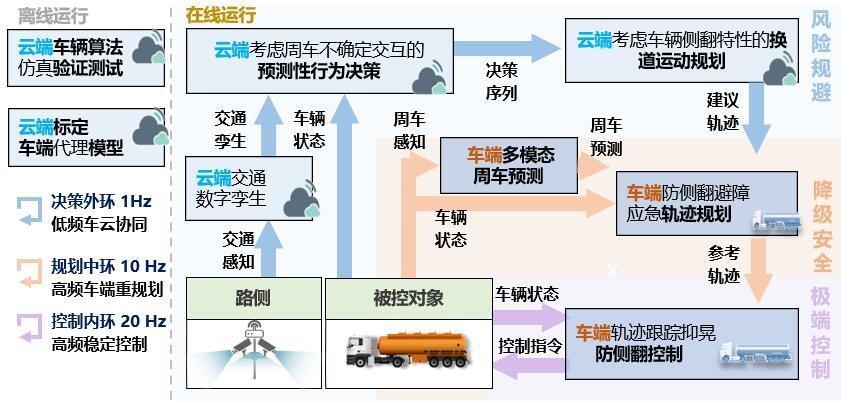
\includegraphics[width=0.92\textwidth]{fig/chap2/safe_arch.jpg}
  \caption{Vehicle--cloud collaborative predictive planning and anti-rollover control framework. The cloud side provides long-horizon predictive planning, the vehicle-side planner provides emergency trajectory replanning, and the high-frequency controller enforces trajectory tracking, sloshing suppression, and rollover prevention.}
  \label{fig:vc_framework}
\end{figure*}
% TODO: Redraw Fig. \ref{fig:vc_framework} in English for the final submission. The figure should show cloud-side Graphflow prediction and decision-making, vehicle-side emergency planning, high-frequency MPC, information upload/download, and fallback under communication uncertainty.

The overall information flow is shown in Fig.~\ref{fig:vc_framework}. The cloud side receives the ego state, surrounding traffic graph, road topology, and transportation-task information, and outputs a long-horizon driving decision and a rollover-aware reference trajectory. The vehicle-side planner receives the cloud trajectory, local perception, and ego state, and outputs a locally feasible emergency trajectory when needed. The controller receives the selected reference trajectory and measured or estimated vehicle--liquid states, and outputs steering, differential braking, and speed commands. This structure follows the principle that the cloud reduces the probability of entering dangerous interactions, the vehicle-side planner preserves feasibility when the cloud guide is no longer safe, and the controller forms the final anti-rollover safety layer.

The main contributions are summarized as follows:
\begin{itemize}
  \item A vehicle--cloud collaborative predictive planning and anti-rollover control framework is proposed for autonomous tank trucks, integrating long-horizon cloud-side risk anticipation with vehicle-side real-time stability protection.
  \item A Graphflow-based cloud-side predictive planning module is developed to represent large-scale highway traffic as a directed graph, model long-horizon stochastic interaction, and support reinforcement-learning decision-making through a learned world model.
  \item A vehicle-side planning and high-frequency control strategy is formulated by combining dual-scenario contingency replanning, coupled liquid--vehicle dynamics, and multi-constraint MPC for trajectory tracking, sloshing suppression, and rollover prevention.
  \item The proposed method is validated through traffic simulation, high-fidelity vehicle--liquid co-simulation, and scaled tank-truck experiments.
\end{itemize}

The remainder of this paper is organized as follows. Section~II formulates the vehicle--cloud collaborative anti-rollover problem. Section~III presents the cloud-side predictive planning method. Section~IV introduces vehicle-side emergency planning and high-frequency anti-rollover control. Section~V reports simulation and experimental validation. Section~VI concludes the paper, and the Appendix provides additional modeling and implementation details.


\section{Problem Formulation}

\subsection{Vehicle-Cloud Collaborative Anti-Rollover Workflow}

The considered system consists of one autonomous tank truck, surrounding human-driven or automated vehicles, roadside sensing units, and a cloud-side predictive planning service. The target operating domain is a low-penetration highway environment in which the cloud can provide wide-area predictive guidance, but the ego vehicle must retain an independent safety loop. The hierarchy is organized as three nested safety layers. The cloud-side outer loop reduces induced risks by anticipating long-horizon traffic interactions. The vehicle-side planning loop provides degraded-safety fallback when cloud guidance is unavailable or locally unsafe. The high-frequency control loop suppresses state risks caused by roll motion, liquid sloshing, and actuator-limited maneuvers. The ego vehicle is assumed to have onboard perception, localization, state estimation, trajectory replanning, and actuator-level control capability. The cloud-side service is assumed to have access to road topology, fused surrounding-vehicle states, and the ego state through vehicle-road-cloud communication.

At discrete cloud-planning time $k_c$, the cloud constructs a directed traffic graph
\begin{equation}
  \mathcal{G}_{k_c}=(\mathcal{V}_{k_c},\mathcal{E}),
\end{equation}
where $\mathcal{V}_{k_c}$ contains road-node static attributes, surrounding-vehicle dynamic attributes, ego occupancy, and risk-field features, and $\mathcal{E}$ contains road-topology and lane-connectivity attributes. The cloud-side input is
\begin{equation}
  \mathcal{I}_c=\{\mathcal{G}_{k_c},\mathcal{M},x_e(k_c),\mathcal{R}_{nav}\},
\end{equation}
where $\mathcal{M}$ is the road topology, $x_e$ is the ego state, and $\mathcal{R}_{nav}$ is the route or transportation-task constraint. The cloud-side output is
\begin{equation}
  \mathcal{O}_c=\{d_c,\tau_c\},
\end{equation}
where $d_c$ is a long-horizon driving decision, including acceleration and lane-change intention, and $\tau_c=\{r_i^c\}_{i=1}^{N_c}$ is a rollover-aware reference trajectory.

The vehicle-side planning layer receives $\tau_c$, local perception $\mathcal{P}_v$, and the current ego state. It either accepts the cloud trajectory or generates a local emergency trajectory
\begin{equation}
  \tau_v=\{r_i^v\}_{i=1}^{N_v}
\end{equation}
when any of the following events occurs: a sudden obstacle is detected, the cloud trajectory becomes locally infeasible, the predicted rollover index approaches the safety boundary, or the cloud message is delayed, lost, or inconsistent with local perception. The high-frequency control layer tracks the selected trajectory $\tau_r\in\{\tau_c,\tau_v\}$ and outputs steering, braking, and speed commands
\begin{equation}
  u=[\delta,\ p_{brk}^{L1},\ p_{brk}^{R1},\ p_{brk}^{L2},\ p_{brk}^{R2},\ v_{des}]^T.
\end{equation}

\begin{table}[t]
  \centering
  \caption{Layered Information Flow and Time Scale}
  \label{tab:workflow_timescale}
  \begin{tabularx}{\linewidth}{p{0.21\linewidth}p{0.21\linewidth}p{0.26\linewidth}X}
    \toprule
    Layer & Typical rate & Main input & Main output \\
    \midrule
    Cloud-side predictive planning & 1--2 Hz & Traffic graph, road topology, ego state & Long-horizon decision and rollover-aware reference \\
    Vehicle-side emergency planning & about 10 Hz & Cloud reference, local perception, ego state & Locally feasible emergency trajectory \\
    High-frequency anti-rollover control & 20 Hz or higher & Reference trajectory, vehicle-liquid states & Steering, braking, and speed commands \\
    \bottomrule
  \end{tabularx}
\end{table}

Table~\ref{tab:workflow_timescale} summarizes the three time scales. The cloud horizon is selected to cover slow traffic interaction and lane-change evolution, typically 10--30 s. The vehicle-side emergency planner uses a shorter horizon, typically 5--10 s, to respond to abrupt local hazards and to keep a feasible escape branch when the most dangerous local scenario occurs. The controller uses a horizon of approximately 2--3 s, which covers the dominant liquid-sloshing and roll dynamics. This separation follows the service-time analysis in which cloud-side loops are affected by communication delay and tail latency, while the vehicle-side loop must satisfy emergency response and stability constraints \cite{xionglu2024_CVIS_survay,xuqing2021unreliable,wang2021platoonmpc}.

\subsection{Tank-Truck Rollover Risk Description}

The rollover risk of a tanker truck is driven by road curvature, lateral acceleration, articulation, roll motion, and liquid-sloshing forces. For a generic axle group, the load transfer ratio can be written as
\begin{equation}
  \mathrm{LTR}=\frac{F_z^R-F_z^L}{F_z^R+F_z^L},
  \label{eq:ltr_definition}
\end{equation}
where $F_z^R$ and $F_z^L$ are the right- and left-side vertical tire loads. The condition $|\mathrm{LTR}|=1$ indicates wheel lift-off. Because direct vertical tire-load measurement is difficult in engineering deployment, the controller uses a suspension-force-equivalent rollover index
\begin{equation}
  \mathrm{LTR}_{eql}
  =c_r(-k_{r1}\phi_1-c_1\dot{\phi}_1-k_{r2}\phi_2-c_2\dot{\phi}_2),
  \label{eq:ltr_eql_problem}
\end{equation}
where $\phi_i$ and $\dot{\phi}_i$ denote tractor or trailer roll angle and roll rate, $k_{ri}$ and $c_i$ are suspension roll stiffness and damping, and $c_r$ is a normalization coefficient. In the planning layer, simplified rollover models are used to screen candidate trajectories. In the control layer, $\mathrm{LTR}_{eql}$ is directly included as a constrained MPC output.

The selected trajectory must also account for liquid sloshing. Let $x_l$ denote the equivalent liquid state, including sloshing displacement or pendulum angles and their rates. The coupled tanker-truck state is expressed compactly as
\begin{equation}
  x=[x_v^T,\ x_l^T]^T,
\end{equation}
where $x_v$ contains longitudinal velocity, lateral velocity, yaw states, roll states, articulation-related states, and global pose. The coupled dynamics used by the vehicle-side planner and controller can be written as
\begin{equation}
  x_{k+1}=f(x_k,u_k,w_k),
  \label{eq:coupled_compact}
\end{equation}
where $w_k$ represents road, traffic, and modeling disturbances. Section~IV gives the control-oriented realization of this model.

\subsection{Hierarchical Planning and Control Problem}

The complete vehicle-cloud collaborative problem is formulated as a hierarchical optimization and arbitration problem:
\begin{equation}
  \tau_c^\star,d_c^\star
  =\arg\max_{\tau_c,d_c} \mathbb{E}\left[
  R_c(\mathcal{G}_{0:H_c},d_c,\tau_c)
  \right],
  \label{eq:cloud_problem}
\end{equation}
\begin{equation}
  \tau_v^\star
  =\arg\min_{\tau_v}
  J_v(\tau_v,\tau_c,\mathcal{P}_v)
  \quad
  \mathrm{s.t.}\quad
  g_v(\tau_v,\mathcal{P}_v)\leq 0,
  \label{eq:vehicle_planning_problem}
\end{equation}
\begin{equation}
  U^\star
  =\arg\min_{U}
  J_m(x_0,U,\tau_r)
  \quad
  \mathrm{s.t.}\quad
  g_m(x_0,U,\tau_r)\leq 0.
  \label{eq:mpc_problem_compact}
\end{equation}
In \eqref{eq:cloud_problem}, $R_c$ rewards safety, efficiency, comfort, rule compliance, and route consistency over the cloud prediction horizon $H_c$. In \eqref{eq:vehicle_planning_problem}, $J_v$ penalizes deviation from the accepted cloud guide, obstacle proximity, road-boundary violation, excessive curvature, and predicted rollover risk. In \eqref{eq:mpc_problem_compact}, $J_m$ penalizes tracking error, sloshing motion, rollover-index violation, actuator effort, and control increments.

The corresponding constraints include
\begin{equation}
  |\mathrm{LTR}_{eql,k}| \leq \mathrm{LTR}_{max}+\epsilon_{ltr,k},
  \label{eq:ltr_constraint_problem}
\end{equation}
\begin{equation}
  u_{min}\leq u_k\leq u_{max},\quad
  \Delta u_{min}\leq \Delta u_k\leq \Delta u_{max},
  \label{eq:actuator_constraint_problem}
\end{equation}
\begin{equation}
  r_k\in\mathcal{B}_{road},\quad
  \mathcal{B}_{veh}(r_k)\cap\mathcal{B}_{obs,k}=\emptyset,
  \label{eq:road_obstacle_problem}
\end{equation}
where $\epsilon_{ltr,k}$ is a slack variable for soft rollover constraints, $\mathcal{B}_{road}$ is the drivable road region, $\mathcal{B}_{veh}$ is the swept vehicle boundary, and $\mathcal{B}_{obs,k}$ is the obstacle occupancy set. This hierarchy does not require the cloud to control the vehicle directly. Instead, the cloud shifts risk avoidance earlier in time, the vehicle-side planner preserves a locally feasible fallback trajectory, and the MPC forms the final anti-rollover safety layer even when the selected reference is aggressive or the vehicle is already close to the rollover boundary.


\section{Cloud-Side Predictive Planning}

\subsection{Traffic Graph Representation}

Cloud-side predictive planning must reason over a larger spatial range than vehicle-side local perception. In the highway scenarios considered here, a passenger car traveling at 120 km/h can cover about 667 m within 20 s. Therefore, the cloud uses a road-centered graph representation rather than a BEV raster. A large BEV image wastes computation on non-road regions, lets irrelevant background semantics dominate the representation at large spatial scales, and may confuse overlapping ramps or viaducts after projection onto a plane. A graph representation stores only reachable road elements, preserves topological connectivity, and scales with the number of road nodes rather than image area, as illustrated in Fig.~\ref{fig:graph_representation}.

\begin{figure}[t]
  \centering
  \subfloat[BEV representation issue\label{fig:bev_problem_journal}]
    {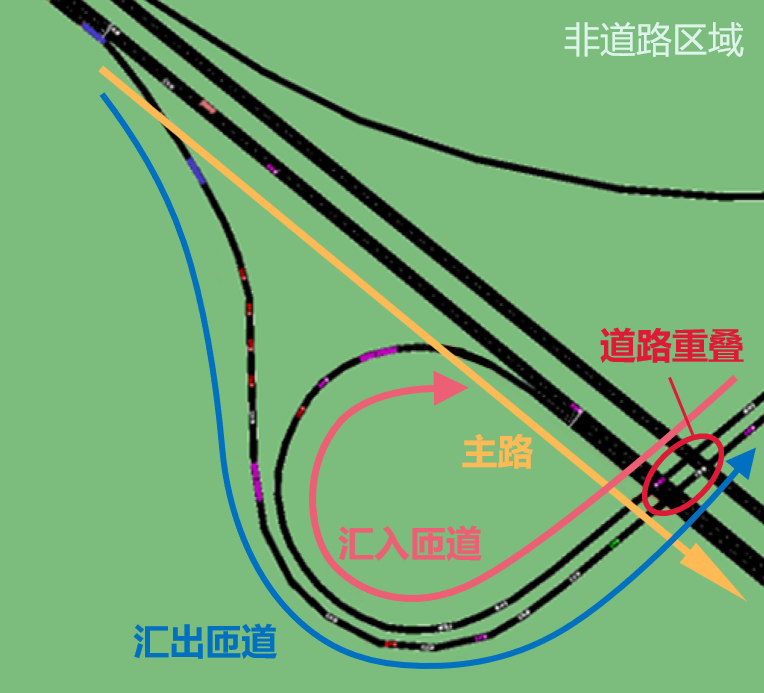
\includegraphics[width=0.44\linewidth]{fig/chap3/bev_problem.png}}
  \subfloat[Directed road graph\label{fig:graph_solution_journal}]
    {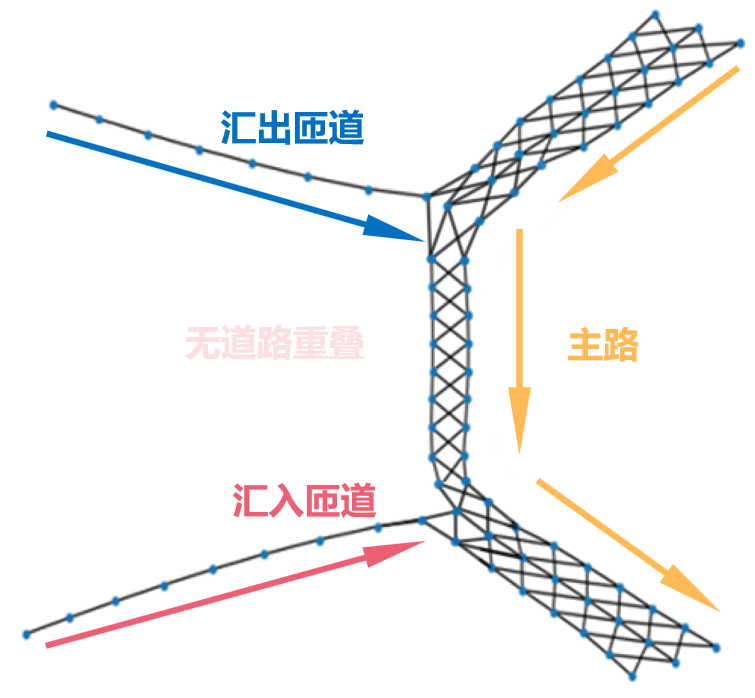
\includegraphics[width=0.44\linewidth]{fig/chap3/graph_solution.png}}
  \caption{Motivation for traffic graph representation in cloud-side predictive planning.}
  \label{fig:graph_representation}
\end{figure}

The road topology is discretized into directed road nodes. For lane-level highway modeling, each lane is discretized longitudinally and laterally, with topology-dependent connections for normal lane sections, merging/diverging sections, and junctions. The resulting graph is
\begin{equation}
  \mathcal{G}=(\mathcal{V},\mathcal{E}),\quad
  \mathcal{V}=F_{stat}\oplus F_{dyn},\quad
  \mathcal{E}=F_{con},
  \label{eq:traffic_graph}
\end{equation}
where $F_{stat}$ contains static road attributes and $F_{dyn}$ contains dynamic traffic attributes. The static node features include node position, lane position type, lane index, edge type, speed limit, and navigation-route indicator. The dynamic node features include surrounding-vehicle occupancy, vehicle type, speed, acceleration, heading, ego occupancy, estimated intention, and a risk-field value. The edge features encode connection type and normalized node distance. Fig.~\ref{fig:graph_features} shows an example.

\begin{figure}[t]
  \centering
  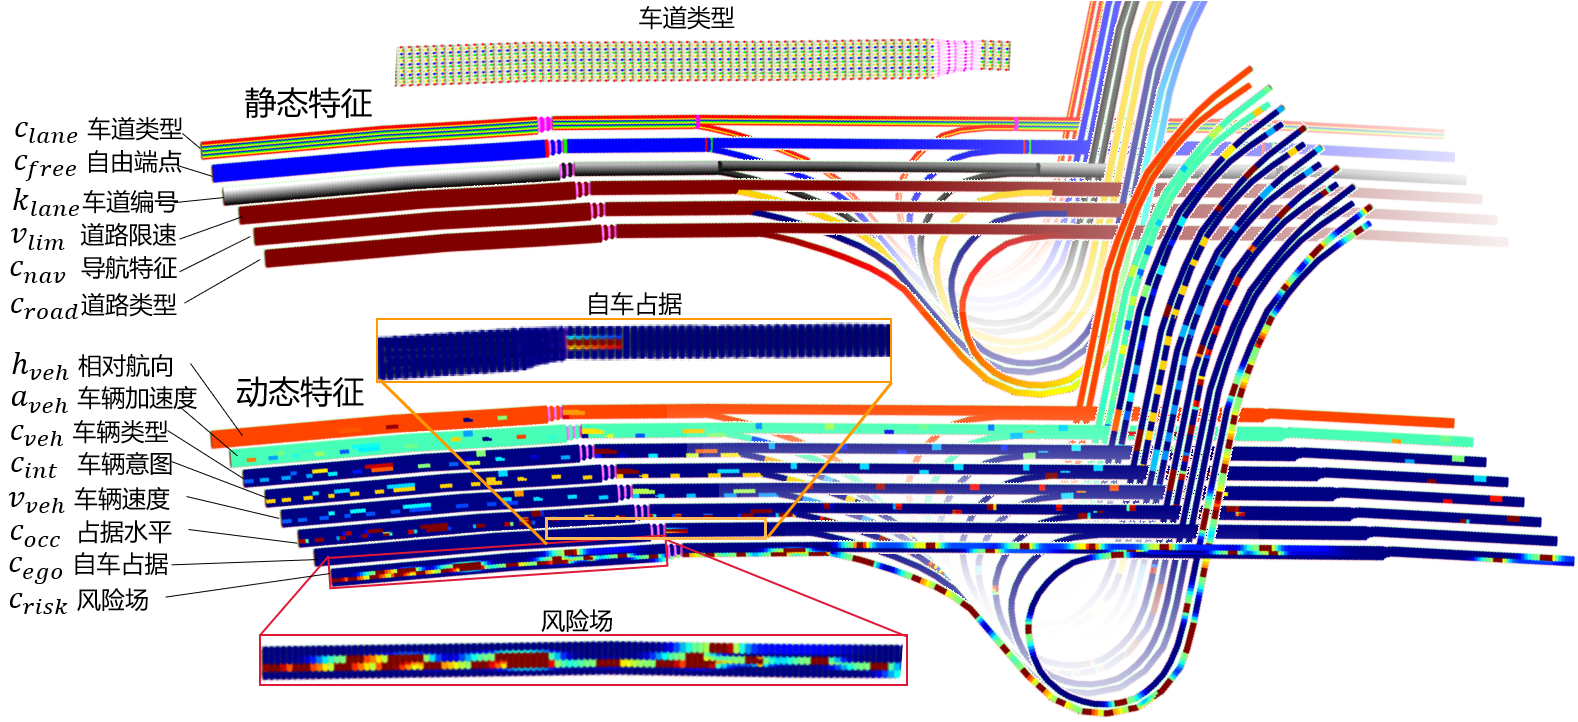
\includegraphics[width=0.95\linewidth]{fig/chap3/feature_example.png}
  \caption{Road-node and edge feature representation for the traffic graph.}
  \label{fig:graph_features}
\end{figure}

The risk field is used to provide a compact local safety prior on the graph. For node $i$ and its longitudinal neighbor $i+k$ in the same lane, the occupancy and speed risks are diffused along forward and backward graph directions:
\begin{equation}
R_{occ}(i,k)=
\begin{cases}
c_{occ}(i)\lambda_f^k, & k>0,\\
c_{occ}(i), & k=0,\\
c_{occ}(i)\lambda_b^{-k}, & k<0,
\end{cases}
\label{eq:r_occ}
\end{equation}
\begin{equation}
R_{spd}(i,k)=
\begin{cases}
c_v^+(i)\lambda_f^k, & k>0,\\
c_v^+(i)+c_v^-(i), & k=0,\\
c_v^-(i)\lambda_b^{-k}, & k<0,
\end{cases}
\label{eq:r_spd}
\end{equation}
where $\lambda_f$ and $\lambda_b$ are exponential decay factors, and $c_v^+$ and $c_v^-$ are normalized relative-speed risk components. The final risk field of target node $j$ is
\begin{equation}
  \begin{aligned}
  c_{risk}(j)=\min\bigg(&
  \sum_{i\in\Omega_b(j)} R_{occ}(i,j-i)\\
  &+\lambda_{spd}R_{spd}(i,j-i),\,1\bigg),
  \end{aligned}
  \label{eq:risk_field}
\end{equation}
where $\Omega_b(j)$ is the set of same-lane source nodes that can contribute risk to node $j$.

\subsection{Graphflow-Based Interactive Prediction}

Graphflow is designed as an autoregressive graph-flow prediction model for long-horizon stochastic interaction. Given historical graph states, the ego action, and time encoding, it predicts the future evolution of dynamic node features over a horizon of 20 s. Unlike deterministic trajectory predictors, Graphflow models how occupancy and risk diffuse over the graph, which is more suitable for cloud-side risk anticipation than precise single-trajectory prediction at long horizons. This formulation also avoids explicitly enumerating all surrounding-vehicle intention combinations, whose strategy tree grows rapidly with the number of vehicles and the decision horizon.

\begin{figure}[t]
  \centering
  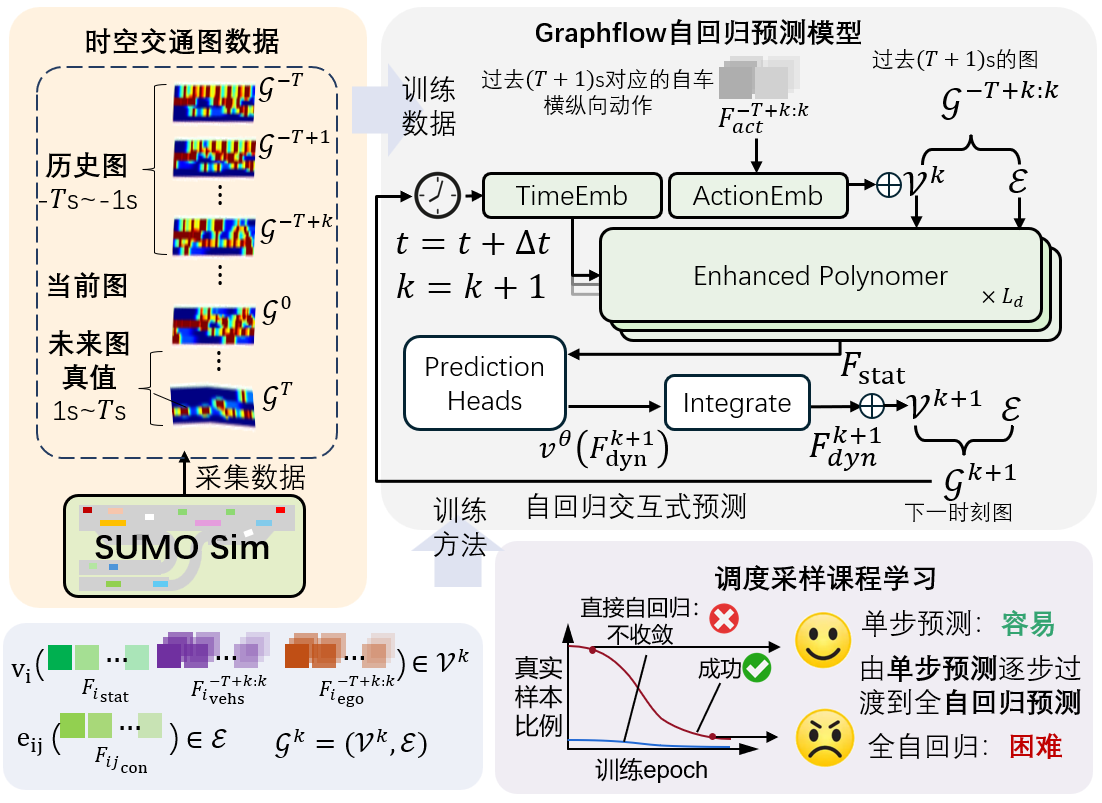
\includegraphics[width=0.95\linewidth]{fig/chap3/graphflow_training.png}
  \caption{Graphflow training and autoregressive graph diffusion.}
  \label{fig:graphflow_training_journal}
\end{figure}

The model input at step $k$ is a spatiotemporal graph
\begin{equation}
  \mathcal{G}_{st}^{k}=
  \left\{F_{stat},F_{dyn}^{k-T:k},\mathcal{E},a_e^k\right\},
  \label{eq:graphflow_input}
\end{equation}
where $a_e^k$ is the ego action used to condition surrounding-vehicle evolution. The graph encoder contains local edge-aware graph attention for neighbor interaction and a global graph attention block for long-range dependency. Time and ego-action encodings are injected into node embeddings. The model outputs a velocity field of dynamic node features:
\begin{equation}
  v_t^{\boldsymbol{\theta}}(F_{dyn}^{t}|\mathcal{G}_{st}^{k}),
  \quad t\in[k,k+1].
  \label{eq:graphflow_velocity}
\end{equation}

The flow-matching objective is used because the training data contain true graph evolution between adjacent time steps. A target velocity field $v_t^{target}$ is obtained by time interpolation and differentiation between $F_{dyn}^k$ and $F_{dyn}^{k+1}$. The conditional flow-matching loss is
\begin{equation}
  \mathcal{L}_{CFM}(\boldsymbol{\theta})=
  \left\|
  v_t^{\boldsymbol{\theta}}(F_{dyn}^{t}|\mathcal{G}_{st}^{k})
  -v_t^{target}(F_{dyn}^{t}|F_{dyn}^{k+1})
  \right\|_2^2.
  \label{eq:cfm_loss}
\end{equation}
The predicted next graph is obtained with one-step numerical integration:
\begin{equation}
  F_{dyn}^{\boldsymbol{\theta},k+1}
  =F_{dyn}^{k}
  +\Delta t\,
  v_t^{\boldsymbol{\theta}}(F_{dyn}^{t}|\mathcal{G}_{st}^{k}).
  \label{eq:graphflow_euler}
\end{equation}
To reduce autoregressive drift, scheduled sampling curriculum learning is adopted \cite{DCRNN2018}. With mini-batch count $N_{batch}$, the teacher-forcing probability is
\begin{equation}
  \epsilon_{SSCL}=
  \frac{\tau_{SSCL}}
  {\tau_{SSCL}+\exp(N_{batch}/\tau_{SSCL})},
  \label{eq:sscl}
\end{equation}
so the model gradually shifts from ground-truth future inputs to its own predicted graph states during training.

\subsection{Long-Horizon Decision-Making}

The cloud-side decision maker uses Graphflow as a learned world model. During training, Graphflow rolls out the traffic graph under candidate ego actions and provides the predicted risk fields used by the reward. During online operation, the trained policy is executed in a receding-horizon manner. Its role is not to directly actuate the vehicle, but to determine a long-horizon behavior guide that reduces interaction-induced rollover triggers. The policy receives the current traffic graph, historical surrounding-vehicle features, and ego features. The ego features include route distance, lane and ramp attributes, ego velocity and heading, lane-change status, neighbor-risk indicators, and navigation intention. Surrounding-vehicle features include existence, relative position, relative velocity, heading, lane relation, vehicle type, route intention, and surrogate safety indicators.

The action is a sequence of acceleration and lane-change commands,
\begin{equation}
  A_c^{k:k+H_c}
  =
  \{a_{des}^{k:k+H_c},\,l_{cmd}^{k:k+H_c}\},
  \label{eq:cloud_action}
\end{equation}
where $l_{cmd}$ is represented continuously during training and mapped to lane-keeping, left-lane-change, or right-lane-change decisions during execution. Surrounding-vehicle parameter and intention uncertainty is estimated from historical cloud twin data using driver and lane-change models. The longitudinal behavior uses a differentiable IDM form \cite{IDM_2020}, while the lane-change probability follows a MOBIL-style utility model \cite{MOBIL_1999}. Bayesian sampling updates the uncertainty of these parameters and intentions when sufficient history or lane-change events are observed.

The policy is trained with PPO. Its reward combines safety, efficiency, comfort/economy, temporal consistency, traffic-rule compliance, and navigation consistency:
\begin{equation}
  r=w_s r_s+w_e r_e+w_c r_c+w_{con}r_{con}+w_r r_r+w_n r_n.
  \label{eq:cloud_reward}
\end{equation}
The safety reward integrates the risk field over ego-occupied nodes and the prediction horizon:
\begin{equation}
  \begin{aligned}
  r_s=&-\frac{1}{H_c Z_o}
  \sum_{t=1}^{H_c}\sum_{\mathbf{v}\in\mathcal{V}}
  \gamma^t c_{risk}(\mathbf{v},t)\mathbb{I}(c_{ego}>\epsilon_o),\\
  Z_o=&\sum_{\mathbf{v}\in\mathcal{V}}\mathbb{I}(c_{ego}>\epsilon_o).
  \end{aligned}
  \label{eq:safety_reward}
\end{equation}
Efficiency rewards speed close to the road limit, comfort penalizes acceleration and lane-change command magnitude, consistency penalizes discontinuity between successive planned action sequences, and rule/navigation rewards penalize speeding and encourage route-consistent lanes. The trained policy outputs the long-horizon driving decision $d_c$.

\subsection{Rollover-Aware Reference Trajectory Generation}

The cloud decision is converted into a continuous trajectory before being transmitted to the vehicle. Longitudinal motion is obtained by integrating the desired acceleration. For lane changes, a sixth-order polynomial is used:
\begin{equation}
\begin{cases}
x(t)=a_0+a_1t+a_2t^2+a_3t^3+a_4t^4+a_5t^5+a_6t^6,\\
y(t)=b_0+b_1t+b_2t^2+b_3t^3+b_4t^4+b_5t^5+b_6t^6.
\end{cases}
\label{eq:sixth_order_traj}
\end{equation}
The initial and terminal position, velocity, and acceleration constraints determine all coefficients except $a_6$ and $b_6$. These remaining degrees of freedom are optimized for rollover awareness. The trajectory lateral acceleration is calculated from curvature:
\begin{equation}
  a_y(t)=
  \frac{\dot{x}(t)\ddot{y}(t)-\dot{y}(t)\ddot{x}(t)}
  {\sqrt{\dot{x}(t)^2+\dot{y}(t)^2}}.
  \label{eq:lateral_acc_from_traj}
\end{equation}
The approximate rollover response is represented by a second-order LTR model:
\begin{equation}
  \ddot{\widetilde{\mathrm{LTR}}}
  +2\zeta\omega_n\dot{\widetilde{\mathrm{LTR}}}
  +\omega_n^2\widetilde{\mathrm{LTR}}
  =a_y(t).
  \label{eq:approx_ltr_model}
\end{equation}
The cloud-side trajectory optimization is
\begin{equation}
\begin{aligned}
  \min_{a_6,b_6}\quad &\|\widetilde{\mathrm{LTR}}(t)\|_{\infty}\\
  \mathrm{s.t.}\quad
  &|\delta(t)|\leq\delta_{max},\quad
  |\dot{\delta}(t)|\leq\dot{\delta}_{max},\\
  &\delta(t)=\arctan(L\kappa(t)).
\end{aligned}
\label{eq:cloud_rollover_traj_opt}
\end{equation}
The source thesis reports that, for a liquid tanker parameterization with $\zeta=0.4$ and $\omega_n=1.8$ Hz, the optimized lane-change trajectory becomes asymmetric and reduces the maximum LTR by approximately 10--20\% compared with a symmetric fifth-order polynomial under the tested speeds.

\begin{figure}[t]
  \centering
  \subfloat[Rollover response and polynomial optimization\label{fig:ltr_feature_journal}]
    {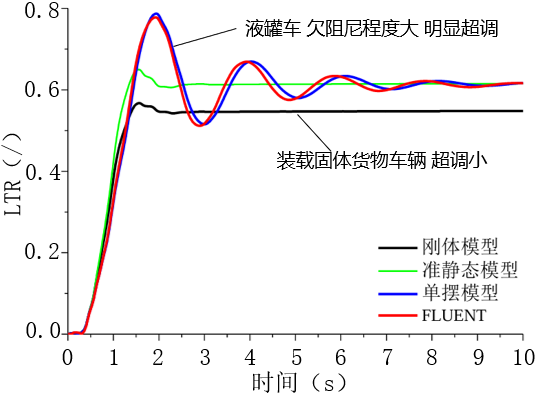
\includegraphics[width=0.92\linewidth]{fig/chap3/ltr_feature.png}}\\
  \subfloat[Solid-cargo and liquid-cargo reference comparison\label{fig:traj_compare_journal}]
    {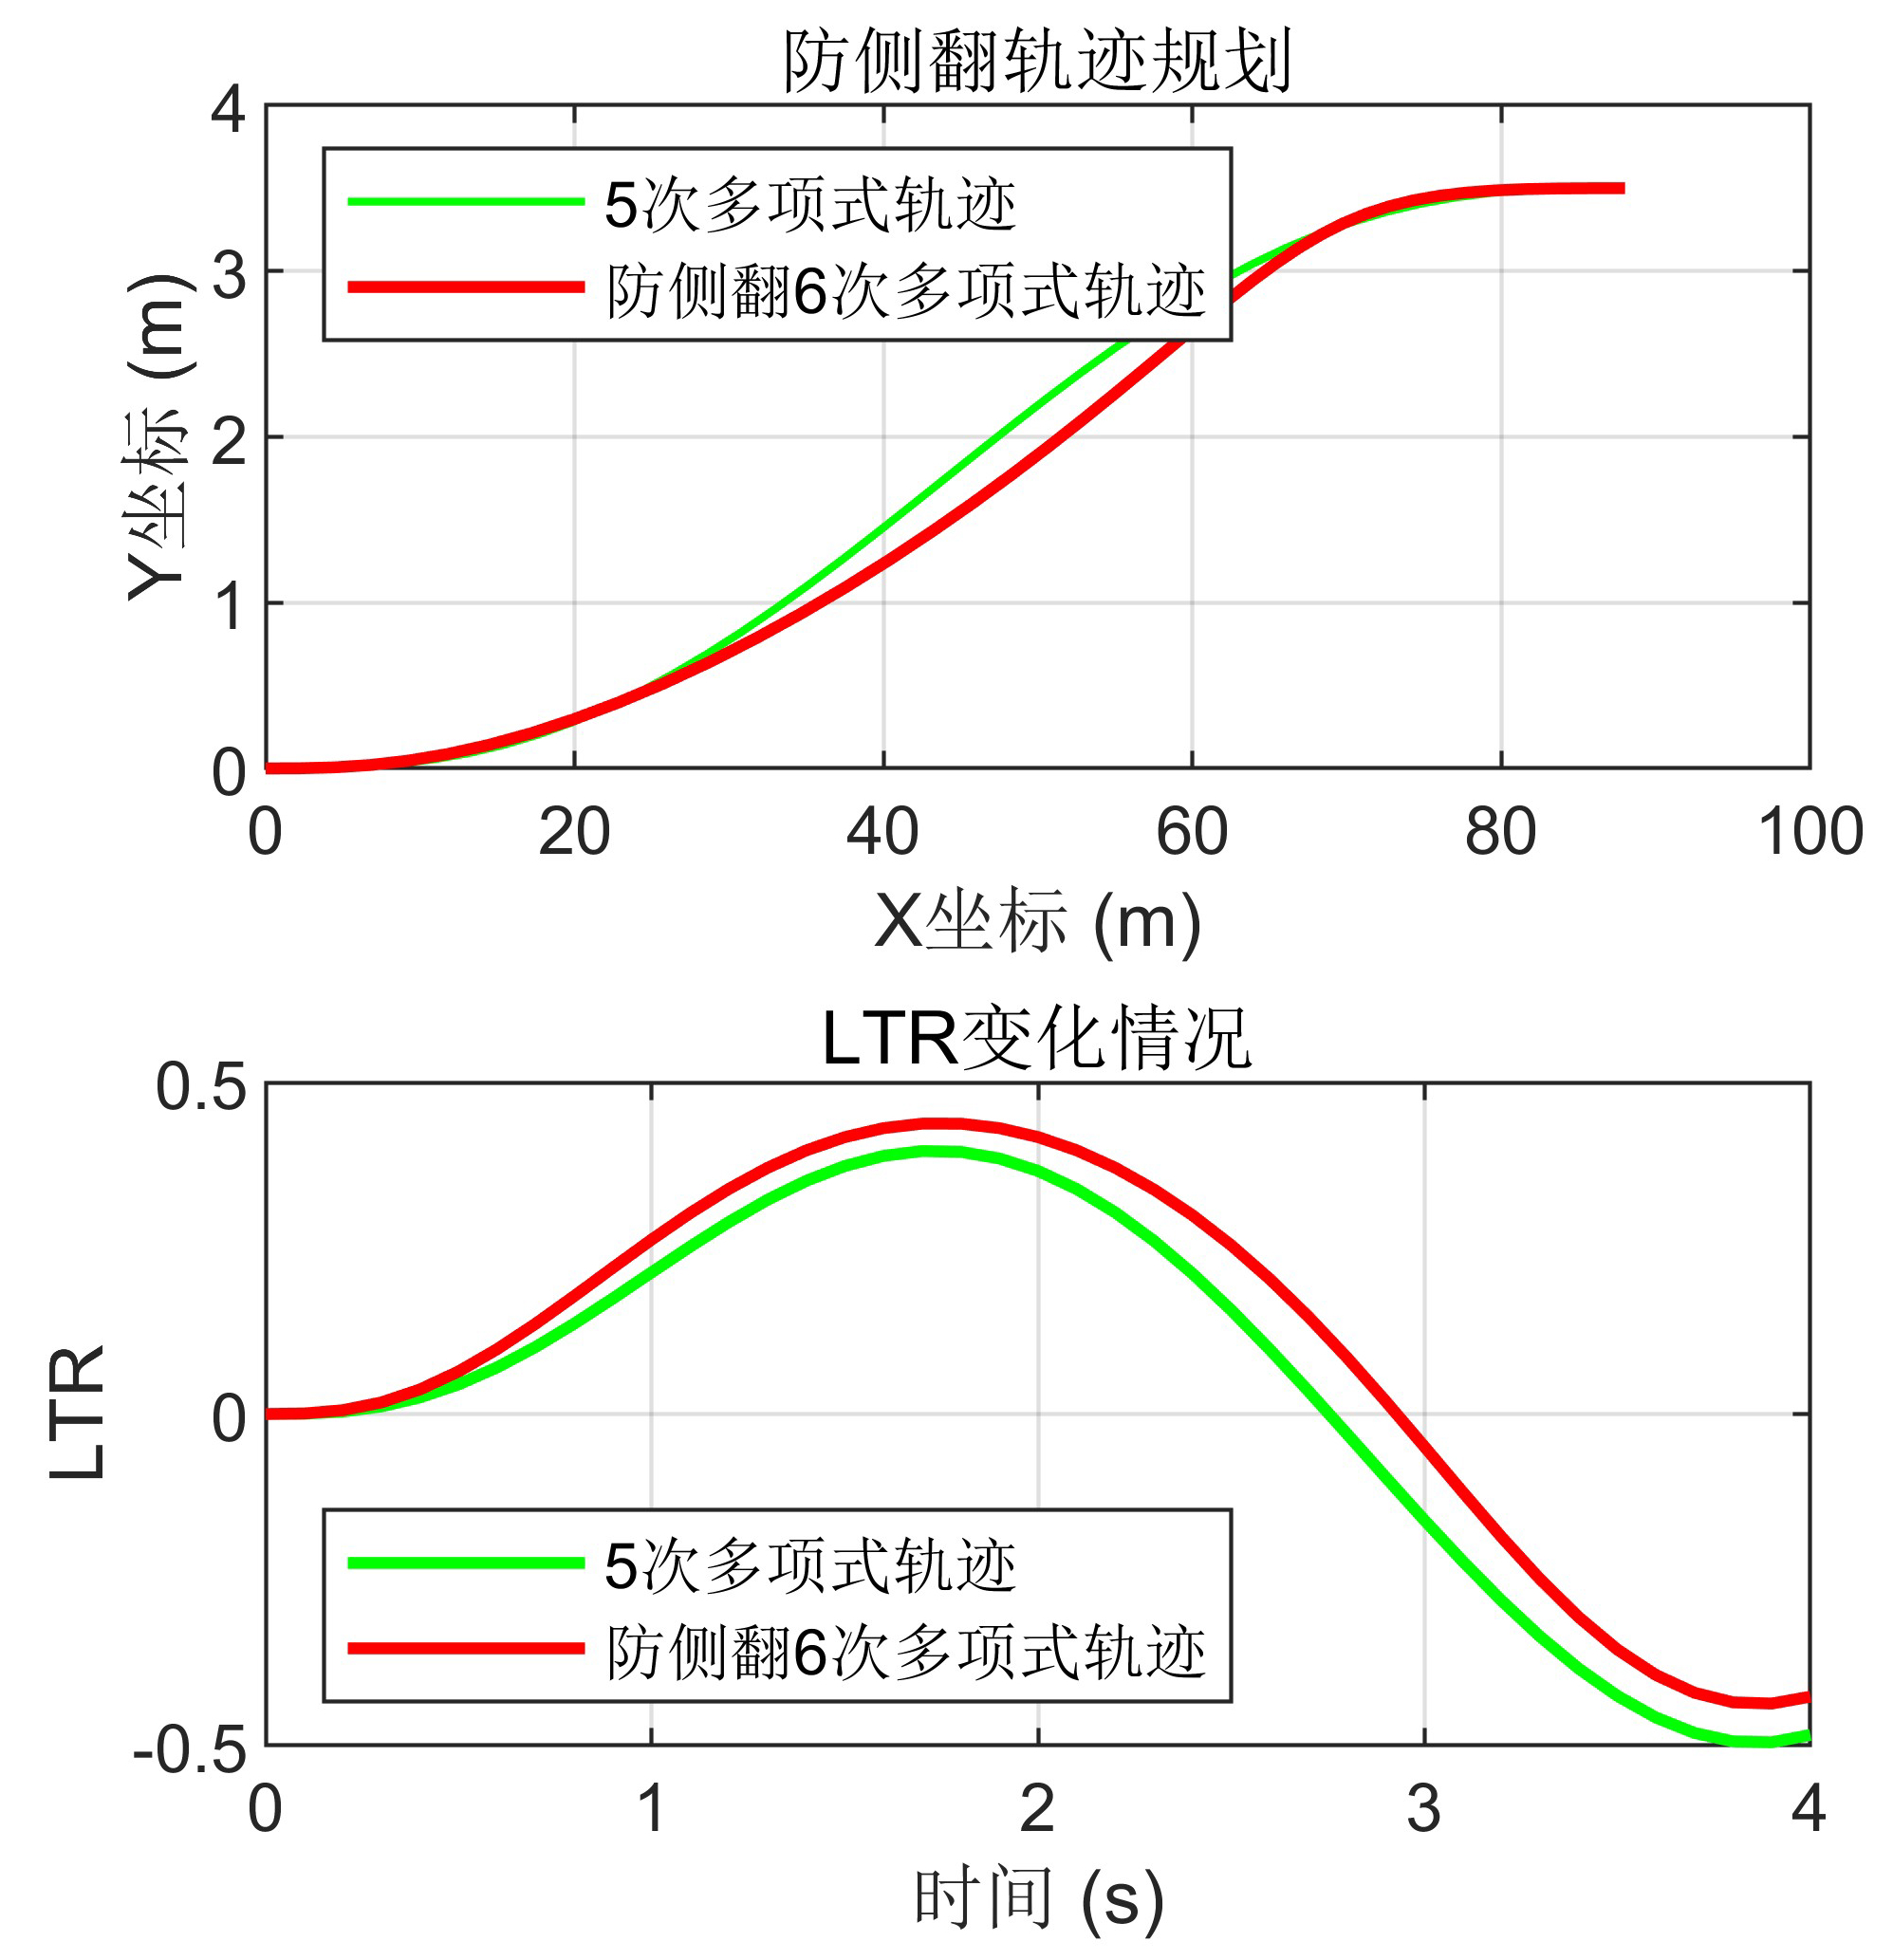
\includegraphics[width=0.92\linewidth]{fig/chap3/liquid_traj.jpg}}
  \caption{Rollover-aware lane-change reference generation on the cloud side.}
  \label{fig:cloud_rollover_reference}
\end{figure}


\section{Vehicle-Side Planning and Anti-Rollover Control}

\subsection{Vehicle-Side Emergency Trajectory Replanning}

The vehicle-side planner is a local safety fallback rather than an independent replacement for cloud-side predictive planning. It is activated when the cloud trajectory conflicts with local perception, a sudden obstacle appears, the rollover margin decreases below a preset threshold, or a cloud message is delayed or inconsistent. The planner uses the cloud trajectory $\tau_c$ as an initial solution and reconstructs a short-horizon trajectory that satisfies local collision, road-boundary, actuator, and rollover constraints.

The planner uses a simplified articulated tanker model for fast prediction. Following the defense-oriented design, the tractor is represented by a kinematic model because it is directly controlled, whereas the trailer keeps speed-dependent amplification and rollover-response terms to preserve high-speed tracking and stability effects. The kinematic part describes the tractor rear-axle position $(X_{1r},Y_{1r})$, tractor heading $\psi_1$, and trailer heading $\psi_2$:
\begin{equation}
\begin{cases}
\dot{X}_{1r}=v_{1x}\cos\psi_1,\\
\dot{Y}_{1r}=v_{1x}\sin\psi_1,\\
\dot{\psi}_1=\frac{v_{1x}}{L_1}\tan\delta,\\
\dot{\psi}_2=K_v\frac{v_{1x}}{L_2}
\left(\frac{L_h}{L_1}\tan\delta\cos\gamma_g+\sin\gamma_g\right),
\end{cases}
\label{eq:vehicle_planning_model}
\end{equation}
where $\gamma_g=\psi_1-\psi_2$ is the articulation angle and $K_v$ is a speed-dependent trailer amplification factor that approximates high-speed tire-slip effects. A low-order linear rollover model is appended to predict LTR under candidate trajectories.

To reduce the number of interaction cases, local multimodal predictions of surrounding vehicles are screened against the cloud reference. For each predicted surrounding-vehicle trajectory $\tau_i^j$, the planner constructs its swept occupancy $\sigma_{\tau_i^j}$ and checks its earliest intersection with the swept occupancy of $\tau_c$. The vehicle whose trajectory first intersects the cloud reference is selected as the key vehicle. The planner then builds two representative scenarios: the most probable scenario $S_\alpha$ and the most dangerous scenario $S_\beta$ that includes the key vehicle's conflicting mode above a probability threshold.

\begin{figure}[t]
  \centering
  \subfloat[Key vehicle selection\label{fig:key_vehicle_selection}]
    {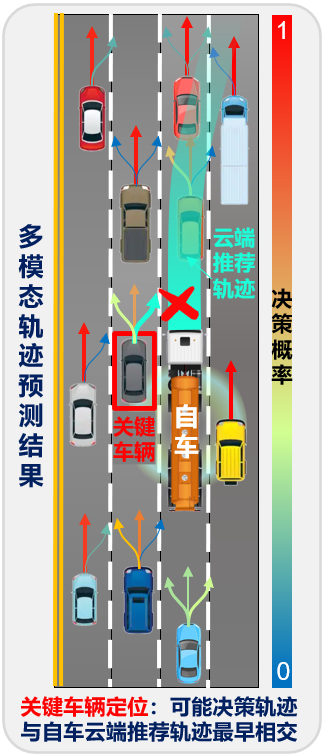
\includegraphics[width=0.31\linewidth]{fig/chap3/scenario_selection1.png}}
  \subfloat[Dual-scenario construction\label{fig:dual_scenario_construction}]
    {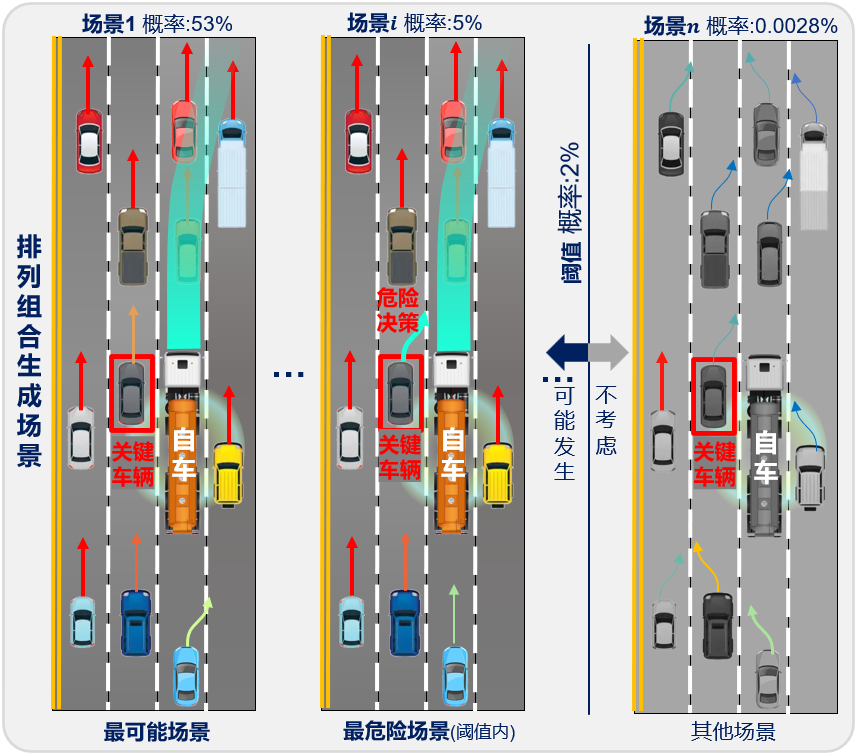
\includegraphics[width=0.63\linewidth]{fig/chap3/scenario_selection2.png}}
  \caption{Vehicle-side emergency scenario screening based on the cloud reference trajectory.}
  \label{fig:vehicle_emergency_scenarios}
\end{figure}

The emergency trajectory is solved with constrained iterative LQR (CILQR). A nominal optimal-control problem is
\begin{equation}
\begin{aligned}
\min_{u_{0:N_p-1}}\quad
& \ell_f(x_{N_p})+\sum_{k=0}^{N_p-1}\ell(x_k,u_k)\\
\mathrm{s.t.}\quad
&x_{k+1}=f_v(x_k,u_k),\quad x_0=x_{start}.
\end{aligned}
\label{eq:cilqr_nominal}
\end{equation}
Obstacle avoidance, road boundaries, steering limits, articulation limits, and rollover limits are introduced through control barrier penalties. For a constraint $c_k(x_k)\leq0$, the penalty is
\begin{equation}
  b_k=q_1\exp(q_2 c_k(x_k)).
  \label{eq:cbf_penalty}
\end{equation}
The rollover constraint is tightened along the prediction horizon to compensate for simplified-model uncertainty:
\begin{equation}
  \mathcal{L}_{lim}(t)=\mathcal{L}_{lim}^{0}\exp(-t/\tau_{decay}).
  \label{eq:ltr_tightened}
\end{equation}
The two scenario trajectories share an initial segment, so the vehicle can preserve performance in $S_\alpha$ while remaining feasible if $S_\beta$ occurs. In implementation, an outer loop adjusts a danger factor according to constraint violation in $S_\beta$, while an inner CILQR loop optimizes the shared-prefix trajectory and the two branches. When the local evidence confirms the dangerous mode, the vehicle switches to the already feasible emergency branch. This contingency structure is the vehicle-side degraded-safety mechanism when the cloud reference no longer provides a sufficient safety margin.

\subsection{Coupled Tank-Truck Dynamics for Control}

The high-frequency controller uses a more detailed control-oriented model than the emergency planner. The model couples a semi-trailer vehicle model with an equivalent liquid-sloshing model. The vehicle part contains tractor lateral, yaw, and roll dynamics, trailer yaw and roll dynamics, longitudinal speed dynamics, and global pose. The liquid part is represented by a linearized double-pendulum (LDP) model whose parameters can be updated from a higher-fidelity sliding telescopic libra (STL) sloshing model. The STL model is introduced to capture longitudinal-lateral coupled sloshing, chamber-to-chamber liquid transfer, and yaw/roll excitation effects that are difficult to express with a conventional two-dimensional pendulum. The STL model is used for high-fidelity rapid simulation and offline or periodic re-linearization; the LDP model is used inside the MPC to preserve real-time solvability.

\begin{figure}[t]
  \centering
  \subfloat[Coordinate definition\label{fig:coord_def_journal}]
    {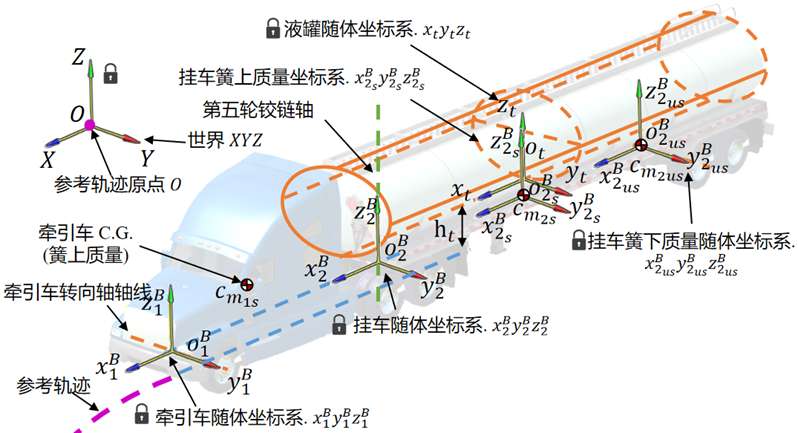
\includegraphics[width=0.64\linewidth]{fig/chap4/coord_def.png}}
  \subfloat[Roll-plane simplification\label{fig:roll_plane_model_journal}]
    {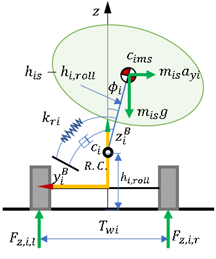
\includegraphics[width=0.28\linewidth]{fig/chap4/trailer_model_lat.png}}\\
  \subfloat[Yaw-plane simplification\label{fig:yaw_plane_model_journal}]
    {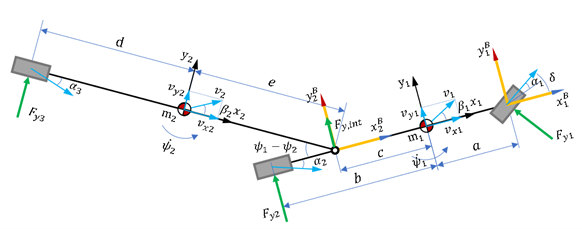
\includegraphics[width=0.95\linewidth]{fig/chap4/trailer_model_lon.png}}
  \caption{Control-oriented coupled semi-trailer tanker-truck model.}
  \label{fig:coupled_vehicle_model}
\end{figure}

The control-oriented state vector is
\begin{equation}
\begin{aligned}
x=&[v_{1y},\dot{\psi}_1,\phi_1,\dot{\phi}_1,
v_{2y},\dot{\psi}_2,\phi_2,\dot{\phi}_2,\\
&\theta_1,\dot{\theta}_1,\theta_2,\dot{\theta}_2,
v_{1x},\psi_1,Y_1,X_1]^T,
\end{aligned}
\label{eq:control_state}
\end{equation}
where the subscripts 1 and 2 denote tractor and trailer, respectively, and $\theta_1,\theta_2$ are the equivalent sloshing angles. The controller input is
\begin{equation}
u=[\delta,\ p_{brk}^{L1},\ p_{brk}^{R1},\ p_{brk}^{L2},\ p_{brk}^{R2},\ v_{des}]^T.
\label{eq:control_input}
\end{equation}
The differential braking variables are grouped by left/right and tractor/trailer axle groups. This input structure allows the controller to coordinate active steering, differential braking, and desired speed.

The continuous-time linearized model at each control step is
\begin{equation}
  \dot{x}=A_c x+B_c u,
  \label{eq:continuous_ltv}
\end{equation}
where $A_c$ and $B_c$ are updated using the current longitudinal speed, roll state, articulation state, and liquid-equivalent parameters. With zero-order hold, the discrete-time model is
\begin{equation}
  x_{k+1}=A_d x_k+B_d u_k.
  \label{eq:discrete_control_model}
\end{equation}
The STL model used for high-fidelity sloshing approximation contains longitudinal-lateral coupled liquid-mass transfer and additional forces/moments. The source thesis reports that an identified STL model predicts 15 s of liquid-force response in about 5 ms in MATLAB and less than 1 ms after C++ compilation, while maintaining the same force/moment trends as CFD over the tested orthogonal excitation cases. For online MPC, a residual reinforcement-learning re-linearization module maps STL states to LDP parameter and state corrections, so the LDP model preserves the dominant sloshing response over the prediction horizon.

\subsection{Multi-Constraint Anti-Rollover MPC}

The MPC is the final safety layer of the proposed vehicle-cloud system. It solves an incremental linear MPC problem to track the selected reference trajectory while suppressing sloshing and preventing rollover. Unlike a pure path-tracking controller, it is expected to reject an unsafe reference by introducing controlled path deviation, speed reduction, and differential braking when the rollover margin becomes small. The output vector is
\begin{equation}
  y=[Y_1,\ X_1,\ \psi_1,\ \dot{\theta}_1,\ \dot{\theta}_2,\ \mathrm{LTR}_{eql},\ v_{1x}]^T.
  \label{eq:mpc_output}
\end{equation}
Absolute position $(Y_1,X_1)$ is used rather than only lateral error, because it better preserves high-order vehicle-liquid dynamics over the 2--3 s control prediction horizon.

For incremental MPC, define
\begin{equation}
  \xi_k=\begin{bmatrix}x_k\\u_{k-1}\end{bmatrix},\quad
  \xi_{k+1}=A\xi_k+B\Delta u_k,\quad
  \eta_k=C\xi_k.
  \label{eq:incremental_mpc_state}
\end{equation}
Stacking the predicted outputs over horizon $N_p$ yields
\begin{equation}
  Y=\Psi\xi_k+\Theta\Delta U,
  \label{eq:stacked_output}
\end{equation}
where $\Delta U=[\Delta u_k^T,\ldots,\Delta u_{k+N_c-1}^T]^T$. The quadratic cost is
\begin{equation}
\begin{aligned}
J=&(Y-Y_r)^TQ_Q(Y-Y_r)+\Delta U^TR_R\Delta U+\rho\epsilon^2\\
=&\frac{1}{2}
\begin{bmatrix}\Delta U\\\epsilon\end{bmatrix}^T
\begin{bmatrix}H&0\\0&\rho\end{bmatrix}
\begin{bmatrix}\Delta U\\\epsilon\end{bmatrix}
+\begin{bmatrix}g\\0\end{bmatrix}^T
\begin{bmatrix}\Delta U\\\epsilon\end{bmatrix}
 + Const.
\end{aligned}
\label{eq:mpc_cost}
\end{equation}
The reference $Y_r$ contains path points, desired heading, desired speed, zero sloshing-rate reference, and a safe rollover-index reference.

The constraints include actuator bounds,
\begin{equation}
  U_{min}\leq U_t+A_t\Delta U\leq U_{max},
  \label{eq:mpc_input_bound}
\end{equation}
input-increment bounds,
\begin{equation}
  \Delta U_{min}\leq\Delta U\leq\Delta U_{max},
  \label{eq:mpc_delta_bound}
\end{equation}
soft output constraints,
\begin{equation}
\begin{cases}
\Pi\Theta\Delta U-\epsilon\leq\Pi(Y_{max}-E),\\
-\Pi\Theta\Delta U-\epsilon\leq\Pi(Y_{min}-E),
\end{cases}
\label{eq:mpc_output_constraint}
\end{equation}
and slack bounds $\epsilon_{min}\leq\epsilon\leq\epsilon_{max}$. Here, $E=\Psi\xi_k$, and $\Pi$ is a constraint-compression mapping. The most important output constraint is
\begin{equation}
  |\mathrm{LTR}_{eql}|\leq \mathrm{LTR}_{max}+\epsilon,
  \label{eq:mpc_ltr_constraint}
\end{equation}
where $\mathrm{LTR}_{max}=0.75$ is used in the simulations and scaled experiments. Sloshing suppression is handled by penalizing and constraining $\dot{\theta}_1$ and $\dot{\theta}_2$, and speed constraints prevent unrealistic compensation between braking and desired-speed commands.

\begin{figure}[t]
  \centering
  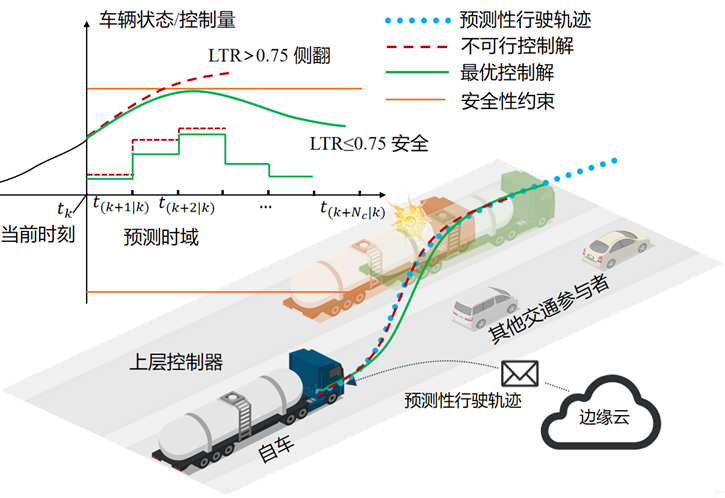
\includegraphics[width=0.78\linewidth]{fig/chap4/mpc_illust.png}
  \caption{Multi-constraint MPC for tracking, sloshing suppression, and rollover prevention.}
  \label{fig:mpc_scheme_journal}
\end{figure}

The resulting QP is solved by qpOASES. To reduce the peak solution time for the high-dimensional state and input space, a moving-block decision compression and constraint-set compression are used. The source thesis reports that this compression has less than 1\% influence on control optimality for the tested setting while reducing peak QP solution time. This acceleration is important because the control layer is the final onboard safety barrier and cannot rely on cloud-side replanning during fast roll and sloshing transients.

\subsection{Real-Time Implementation}

The vehicle-side implementation uses a hierarchical execution logic. At each vehicle-planning cycle, the local planner checks the cloud reference against local perception and predicted rollover margins. If the reference remains safe, the controller tracks $\tau_c$. Otherwise, CILQR generates a local emergency trajectory $\tau_v$, and the controller tracks $\tau_v$. At each control cycle, the state estimator updates vehicle pose, roll states, yaw states, speed, and equivalent liquid states. The LTV model is re-linearized, the MPC QP is solved, and only the first input is applied.

The scaled-vehicle implementation runs the controller at 20 Hz. The source thesis reports an average MPC solution time of 15.4 ms and a peak solution time below 25 ms in model-truck experiments. The controller can therefore serve as the final high-frequency safety layer under the tested experimental conditions.


\section{Validation}

\subsection{Cloud-Side Predictive Planning Evaluation}

The cloud-side module was evaluated in a microscopic traffic simulation constructed from the G15 highway segment between Lianyungang and Yancheng, which is a representative high-risk hazardous-material transport corridor in the thesis study. The route length is about 180 km and includes 15 interchanges with merging and exiting ramps. Four task types were considered: cruising on the mainline, passing an interchange, merging onto the mainline, and exiting from the mainline. Traffic demand was varied from 1000 to 4500 veh/h with a 500 veh/h interval. Interchanges No. 8--15 were used for training data collection, and interchanges No. 1--7 were used for validation. The training data contain approximately 300 GB of SUMO traffic-flow records. With 10 random seeds, the validation set contains 280 simulation runs.

\begin{figure}[t]
  \centering
  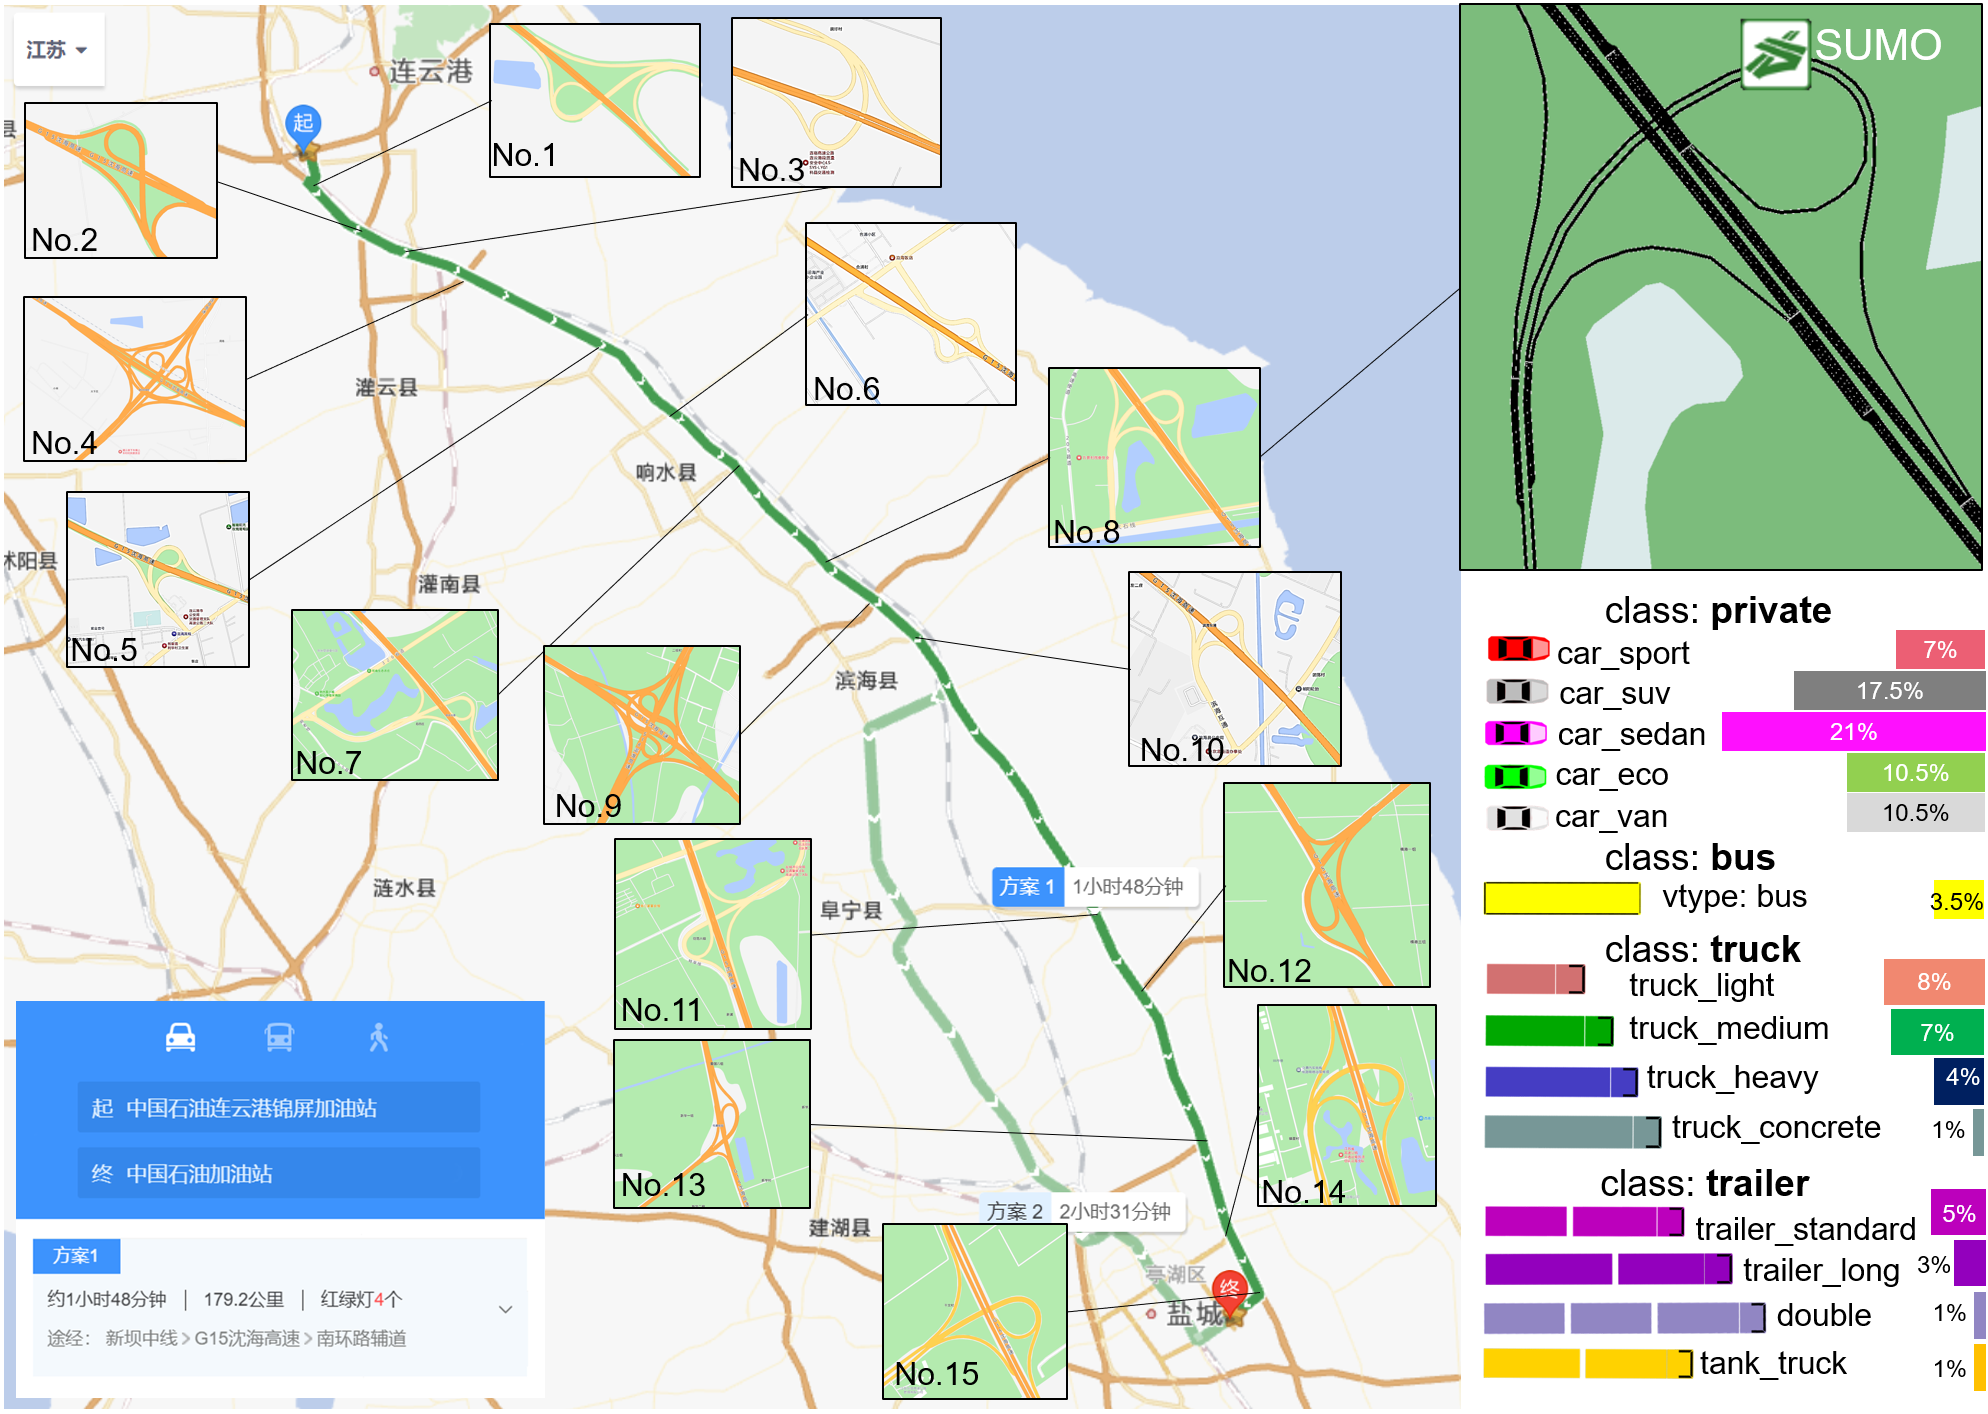
\includegraphics[width=0.95\linewidth]{fig/chap3/sim_place.png}
  \caption{G15 highway traffic simulation environment for cloud-side predictive planning.}
  \label{fig:cloud_sim_place}
\end{figure}

Graphflow was trained for a 20 s prediction horizon. Fig.~\ref{fig:graphflow_validation} reports the training loss and qualitative prediction examples. With scheduled sampling, the ego occupancy feature remains below about 1\% MSE, the risk-field feature remains below about 2\% MSE, and surrounding-vehicle occupancy remains below about 3\% MSE in the reported training process. The qualitative results show that vehicles with stable low-speed motion remain concentrated, while fast vehicles interacting with traffic diffuse into broader low-probability regions. This behavior is consistent with the objective of long-horizon risk anticipation: the model is expected to provide risk-evolution trends rather than exact deterministic trajectories at the end of a 20 s horizon.

\begin{figure}[t]
  \centering
  \subfloat[Training loss\label{fig:train_graphflow_journal}]
    {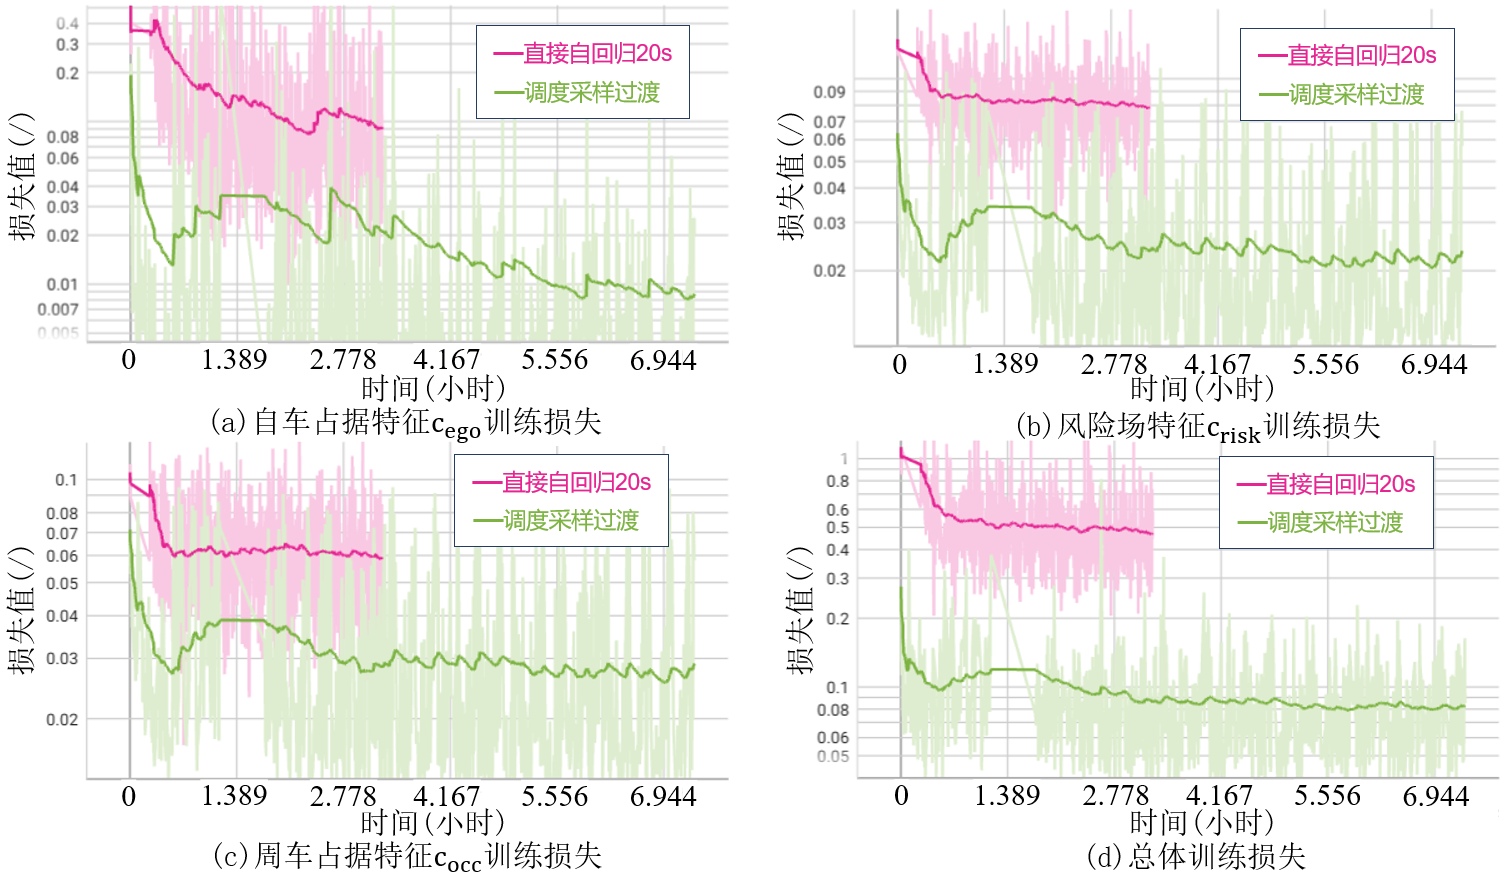
\includegraphics[width=0.92\linewidth]{fig/chap3/train_loss_graphflow.png}}\\
  \subfloat[Straight-road prediction\label{fig:risk_pred1_journal}]
    {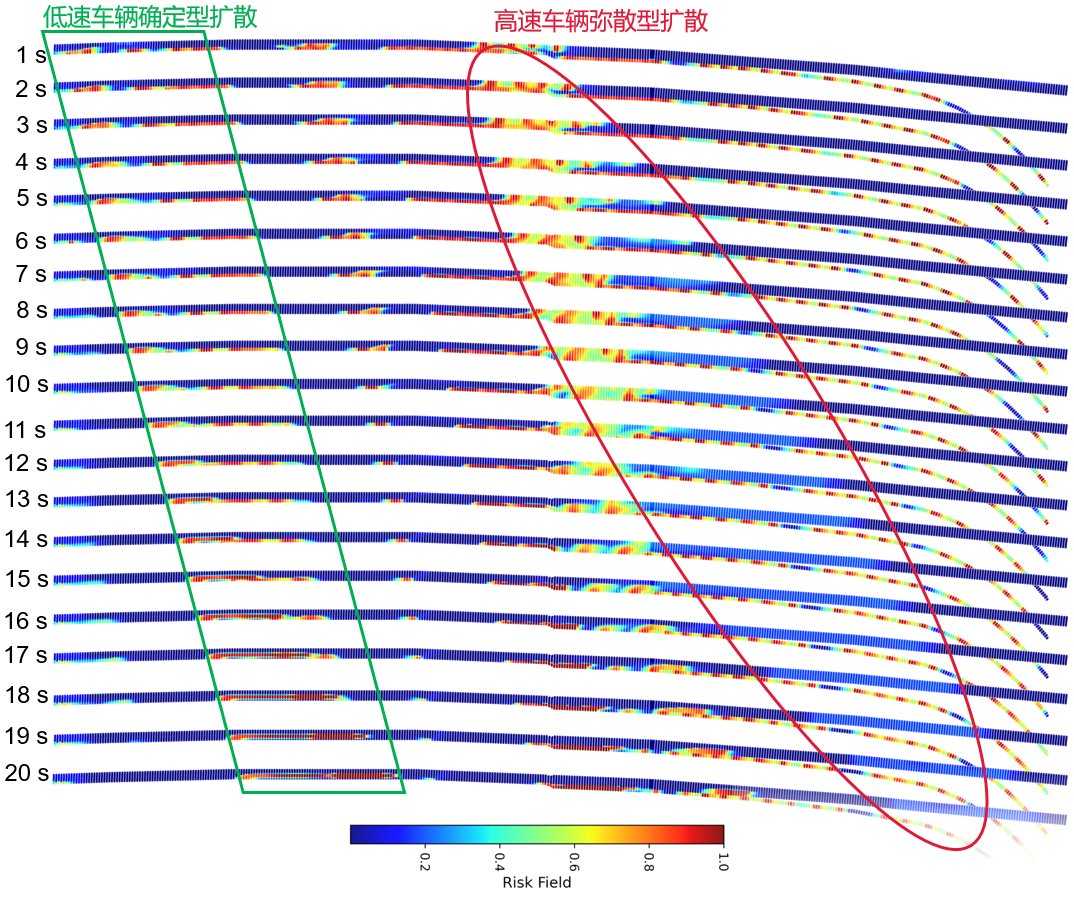
\includegraphics[width=0.92\linewidth]{fig/chap3/risk_pred1.png}}\\
  \subfloat[Interchange prediction\label{fig:risk_pred2_journal}]
    {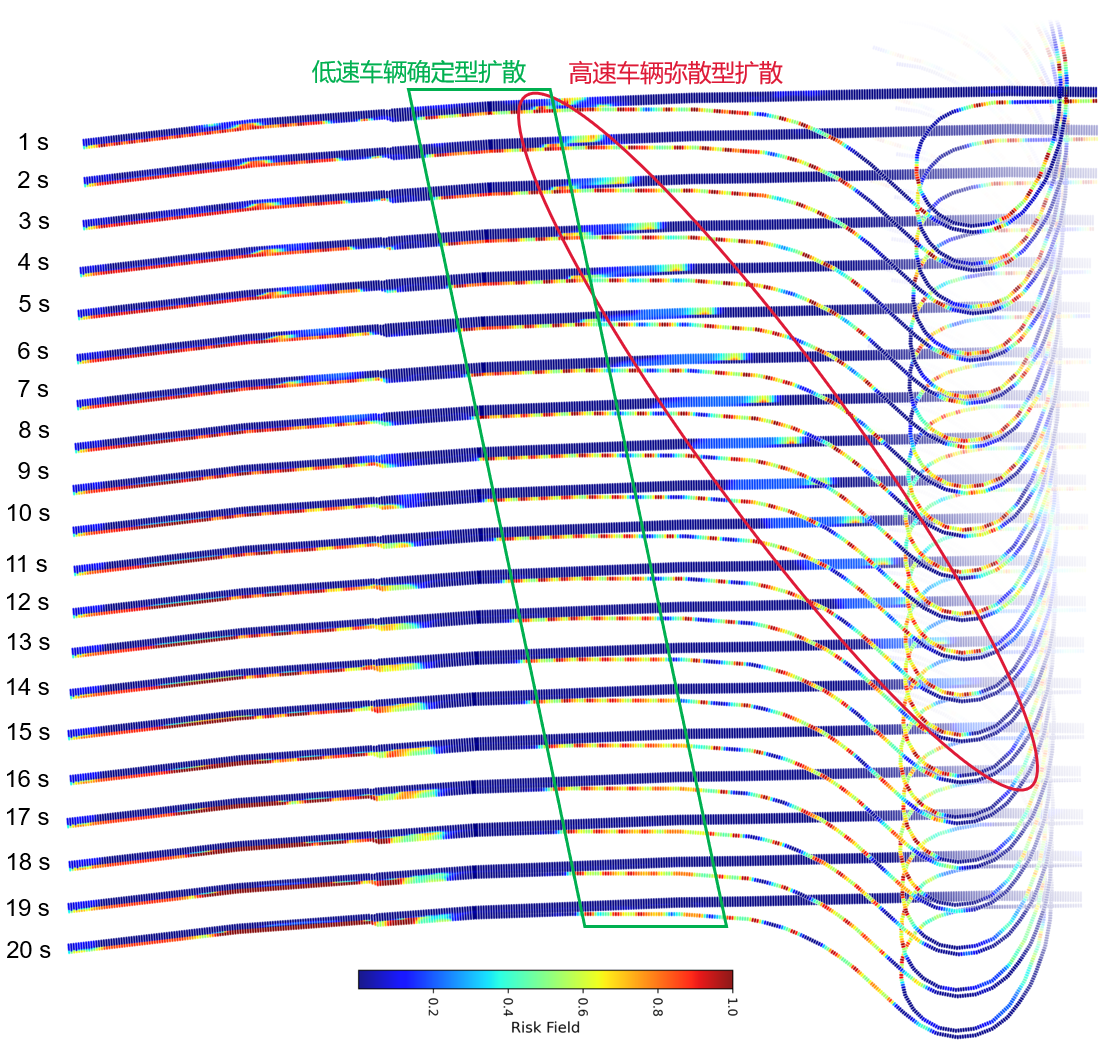
\includegraphics[width=0.92\linewidth]{fig/chap3/risk_pred2.png}}
  \caption{Graphflow training and long-horizon stochastic interaction prediction.}
  \label{fig:graphflow_validation}
\end{figure}

The cloud decision policy was trained with PPO using Graphflow as the world model and then evaluated in SUMO. Two baselines were used: a single-vehicle IDM+MOBIL policy and a decision-tree search baseline with access to the simulation model. The latter is a strong simulation-only baseline because it enumerates ego lane-change choices over a 20 s horizon, with at most three lane changes, and uses near-oracle surrounding-vehicle parameters from SUMO. The source thesis reports that the Graphflow policy achieves total scores close to the decision-tree baseline and higher than the single-vehicle baseline across the validation tasks and traffic demands. Safety improvements are most evident in the trailer-oriented modified emergency index and headway-related risk, while efficiency, comfort/economy, rule compliance, and navigation scores remain comparable to the baselines. This indicates that long-horizon prediction improves safety without forcing overly conservative driving.

\begin{figure}[t]
  \centering
  \subfloat[Total score\label{fig:total_score_journal}]
    {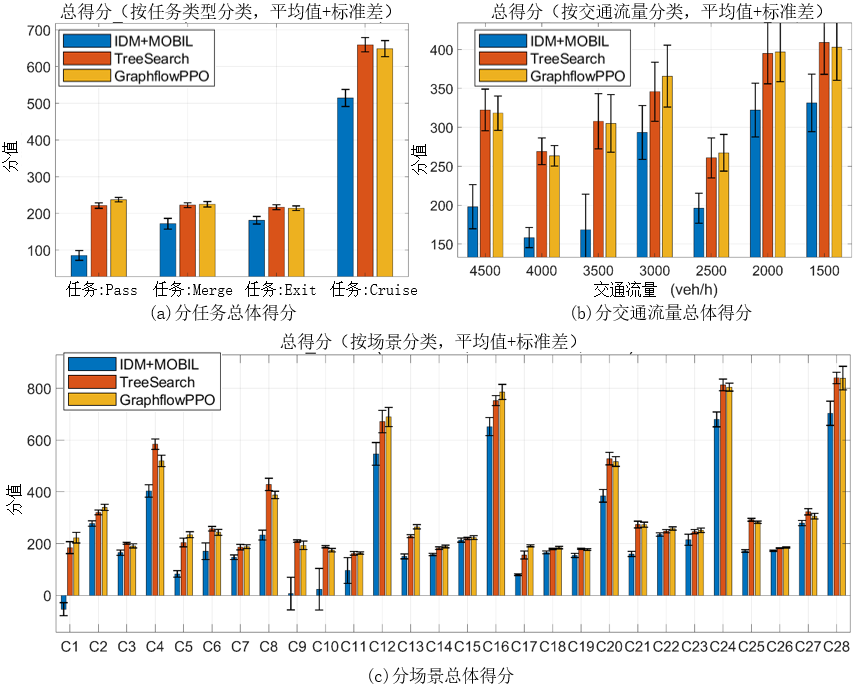
\includegraphics[width=0.92\linewidth]{fig/chap3/total_score.png}}\\
  \subfloat[Safety score\label{fig:r_safe_journal}]
    {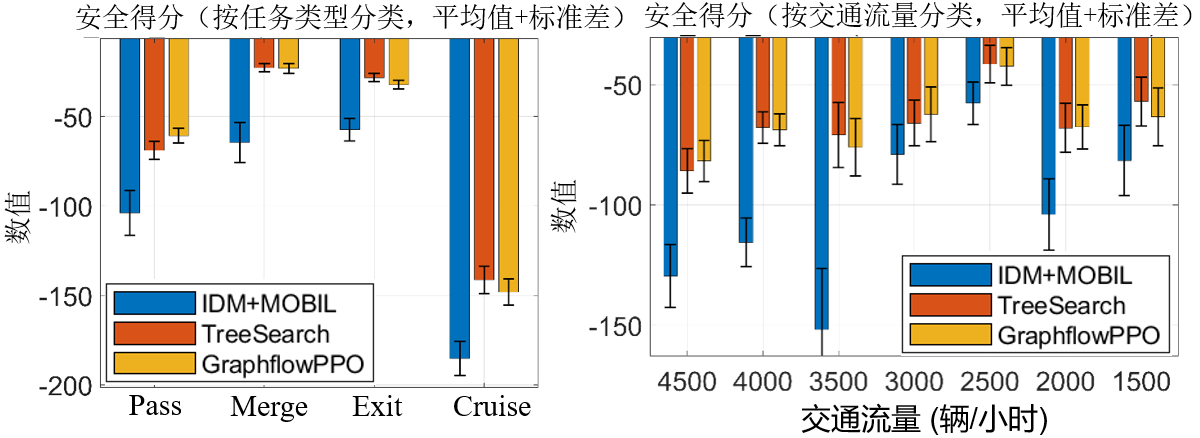
\includegraphics[width=0.92\linewidth]{fig/chap3/r_safe.png}}
  \caption{Cloud-side predictive planning performance on the validation traffic set.}
  \label{fig:cloud_scores}
\end{figure}

A representative cruising case is shown in Fig.~\ref{fig:cloud_case}. The IDM+MOBIL vehicle converges to a locally reasonable but blocked behavior. The tree-search baseline remains in the left lane for a long period, causing prolonged interaction with faster vehicles. The Graphflow policy overtakes, returns to a middle lane, and reduces parallel driving time with faster traffic while maintaining comparable travel progress.

\begin{figure}[t]
  \centering
  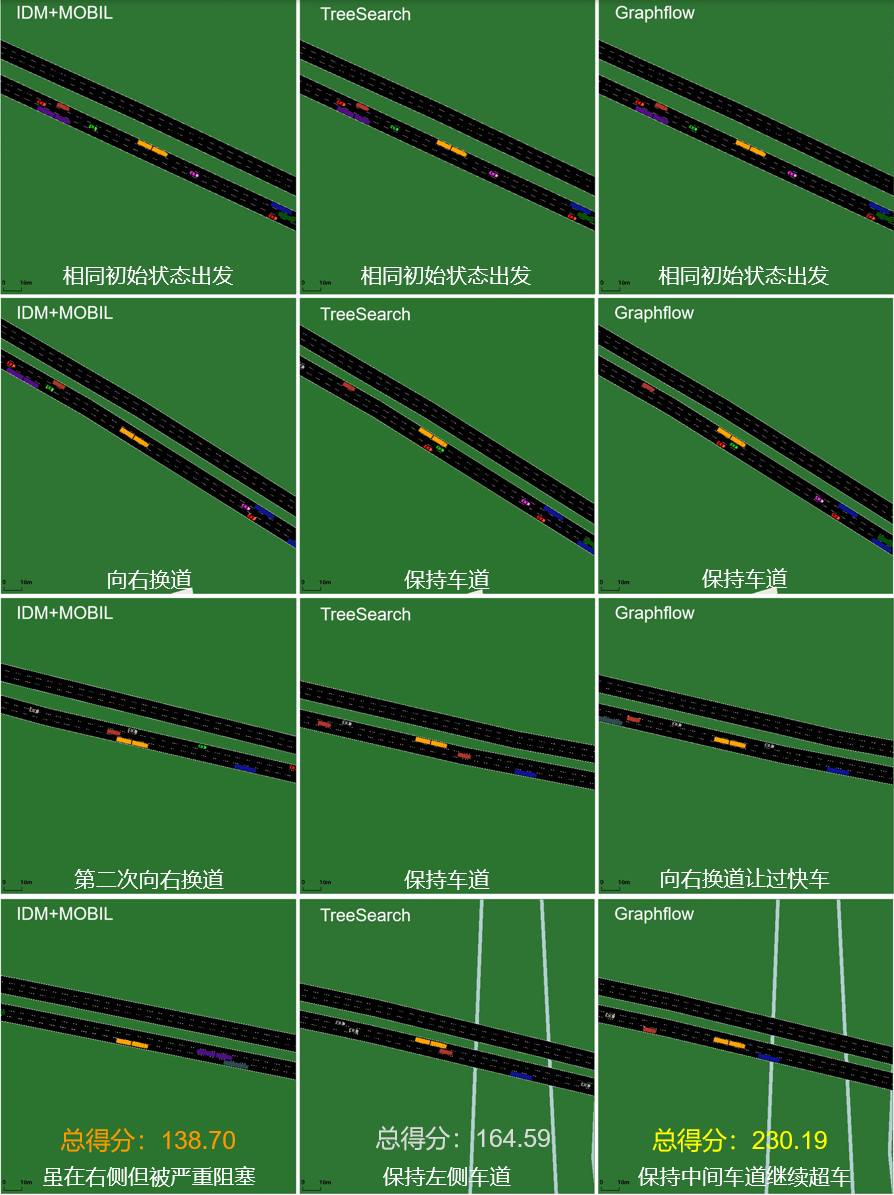
\includegraphics[width=0.95\linewidth]{fig/chap3/example_illust.png}
  \caption{Representative cloud-side planning case comparing IDM+MOBIL, decision-tree search, and Graphflow policy.}
  \label{fig:cloud_case}
\end{figure}

\subsection{Vehicle-Side Planning and Control Evaluation}

Vehicle-side planning was first evaluated in four local emergency cases derived from typical tank-truck accident mechanisms: overtaking with fast rear vehicles, left turning with an oncoming vehicle, high-speed rear approach with a parallel adjacent vehicle, and cruising beside a slow-moving queue. In these cases, the planner uses the cloud reference as the initial solution, identifies the key conflicting vehicle, constructs the most probable scenario $S_\alpha$ and the most dangerous scenario $S_\beta$, and generates a shared-prefix emergency trajectory. The qualitative results in Fig.~\ref{fig:vehicle_planning_cases} show that the planner either preserves the cloud maneuver when the dangerous mode can still be avoided or switches to braking, yielding, shoulder offset, or stopped-lane-change behaviors when the dangerous mode becomes dominant.

\begin{figure}[t]
  \centering
  \subfloat[Fast rear vehicles during overtaking\label{fig:scenario1_journal}]
    {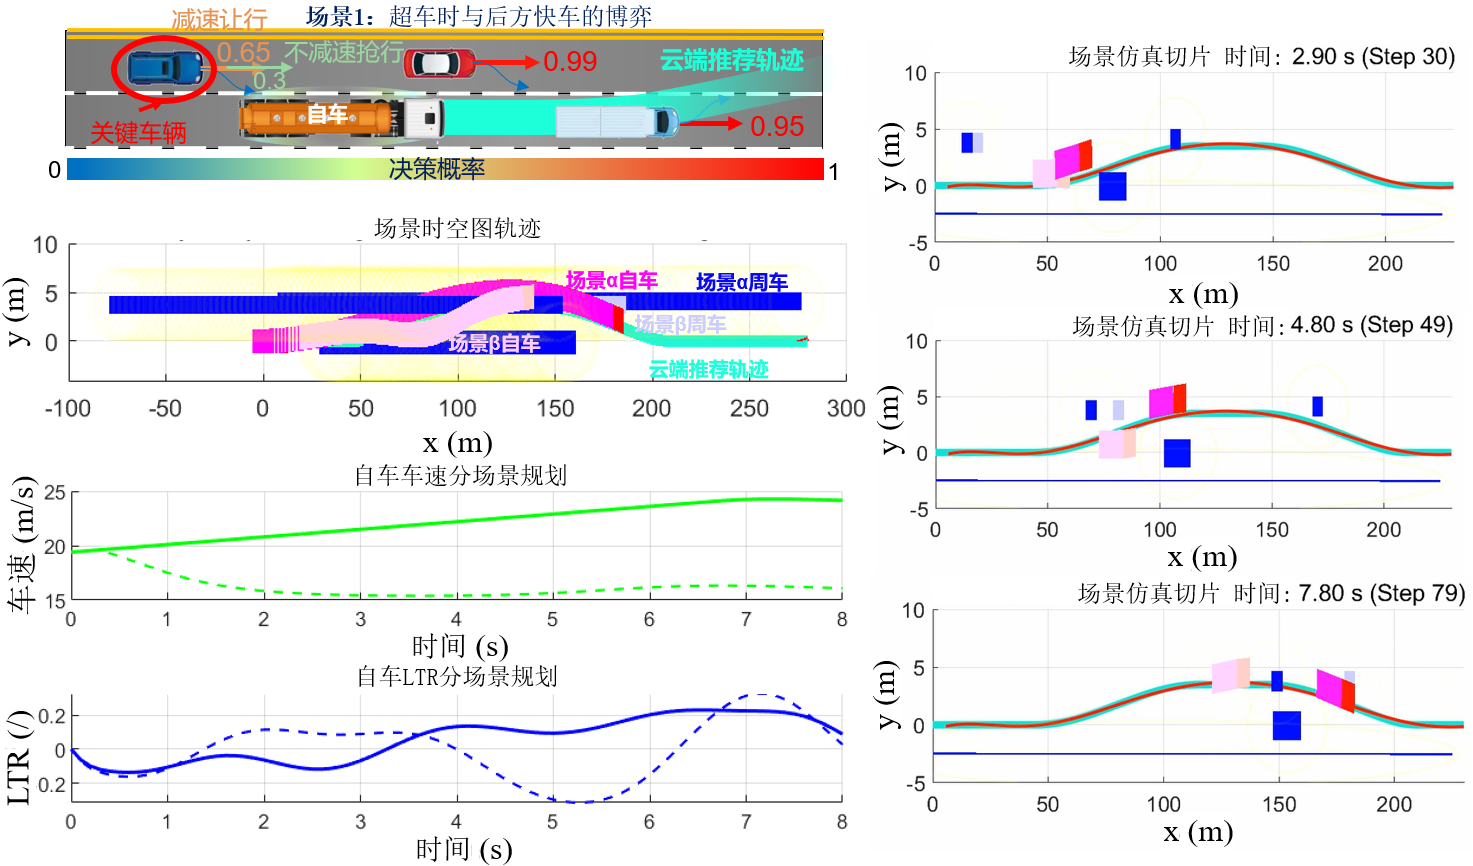
\includegraphics[width=0.48\linewidth]{fig/chap3/scenario1.png}}
  \subfloat[Oncoming vehicle during left turn\label{fig:scenario2_journal}]
    {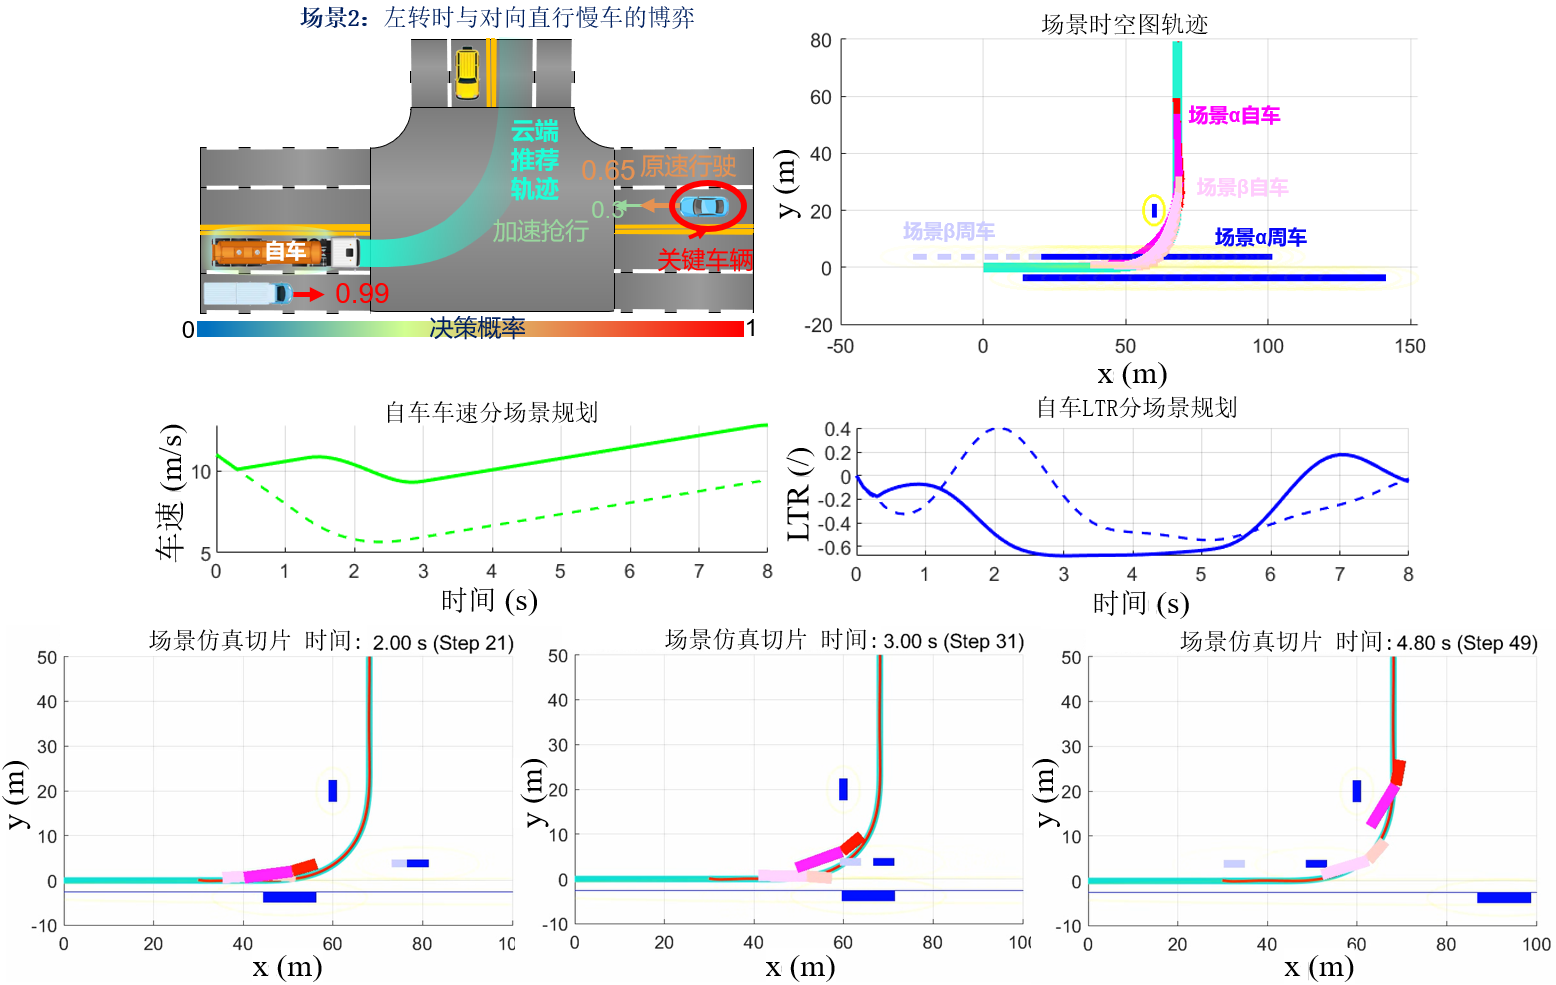
\includegraphics[width=0.48\linewidth]{fig/chap3/scenario2.png}}\\
  \subfloat[Fast rear approach with adjacent parallel vehicle\label{fig:scenario3_journal}]
    {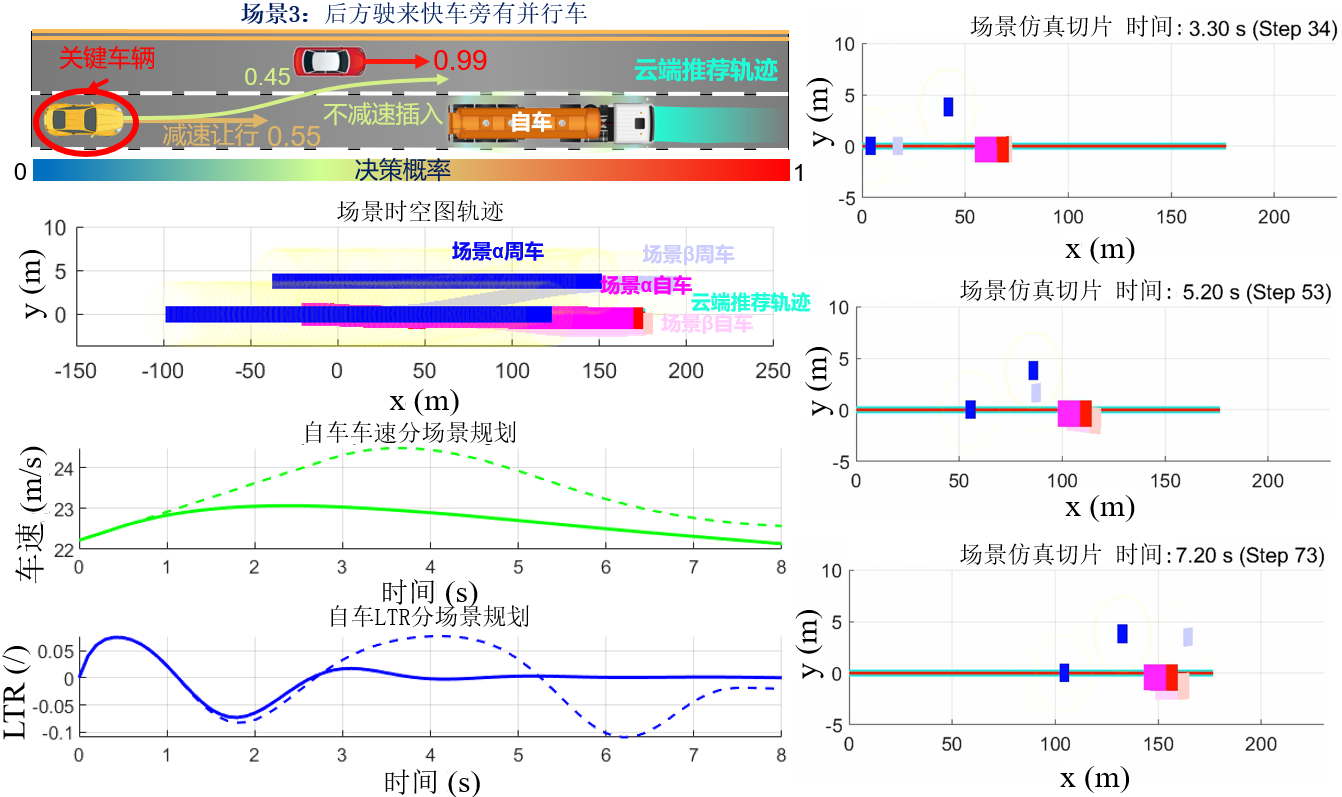
\includegraphics[width=0.48\linewidth]{fig/chap3/scenario3.png}}
  \subfloat[Slow queue beside free lane\label{fig:scenario4_journal}]
    {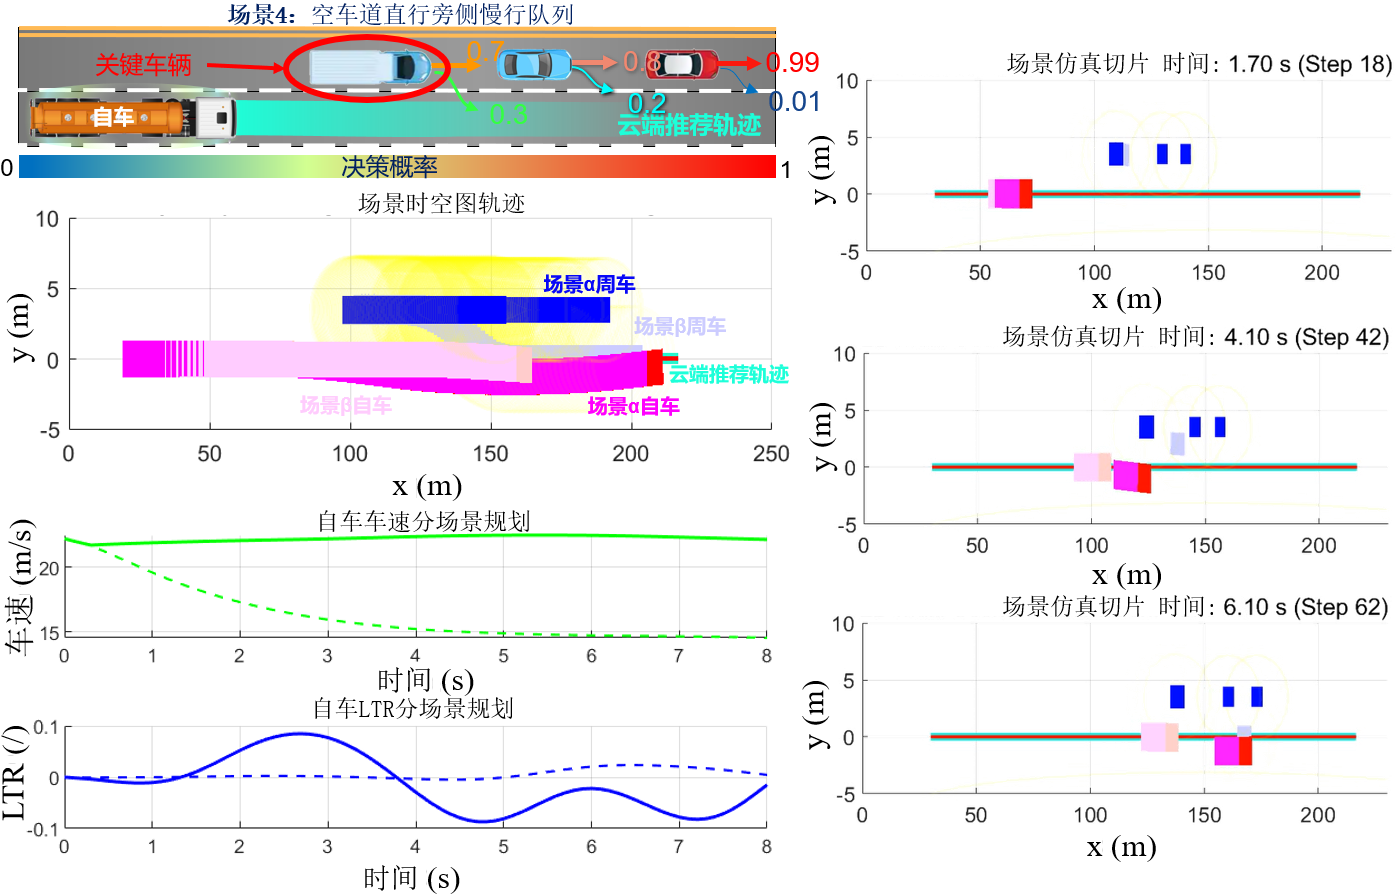
\includegraphics[width=0.48\linewidth]{fig/chap3/scenario4.png}}
  \caption{Vehicle-side emergency replanning cases.}
  \label{fig:vehicle_planning_cases}
\end{figure}

The high-frequency controller was evaluated in a TruckSim--Simulink--StarCCM+ vehicle-liquid co-simulation platform. The platform exchanges vehicle acceleration and angular motion with the CFD tank model and feeds the resulting liquid forces and moments back into the vehicle model. The CFD grid sensitivity analysis reports an average relative force/moment error below 1\% and a peak error below 4\% for the selected mesh setting. The controller frequency is 20 Hz, the co-simulation data exchange interval is 0.005 s, and the liquid filling ratio is 50\%.

\begin{figure}[t]
  \centering
  \subfloat[Co-simulation architecture\label{fig:cosim_arch_journal}]
    {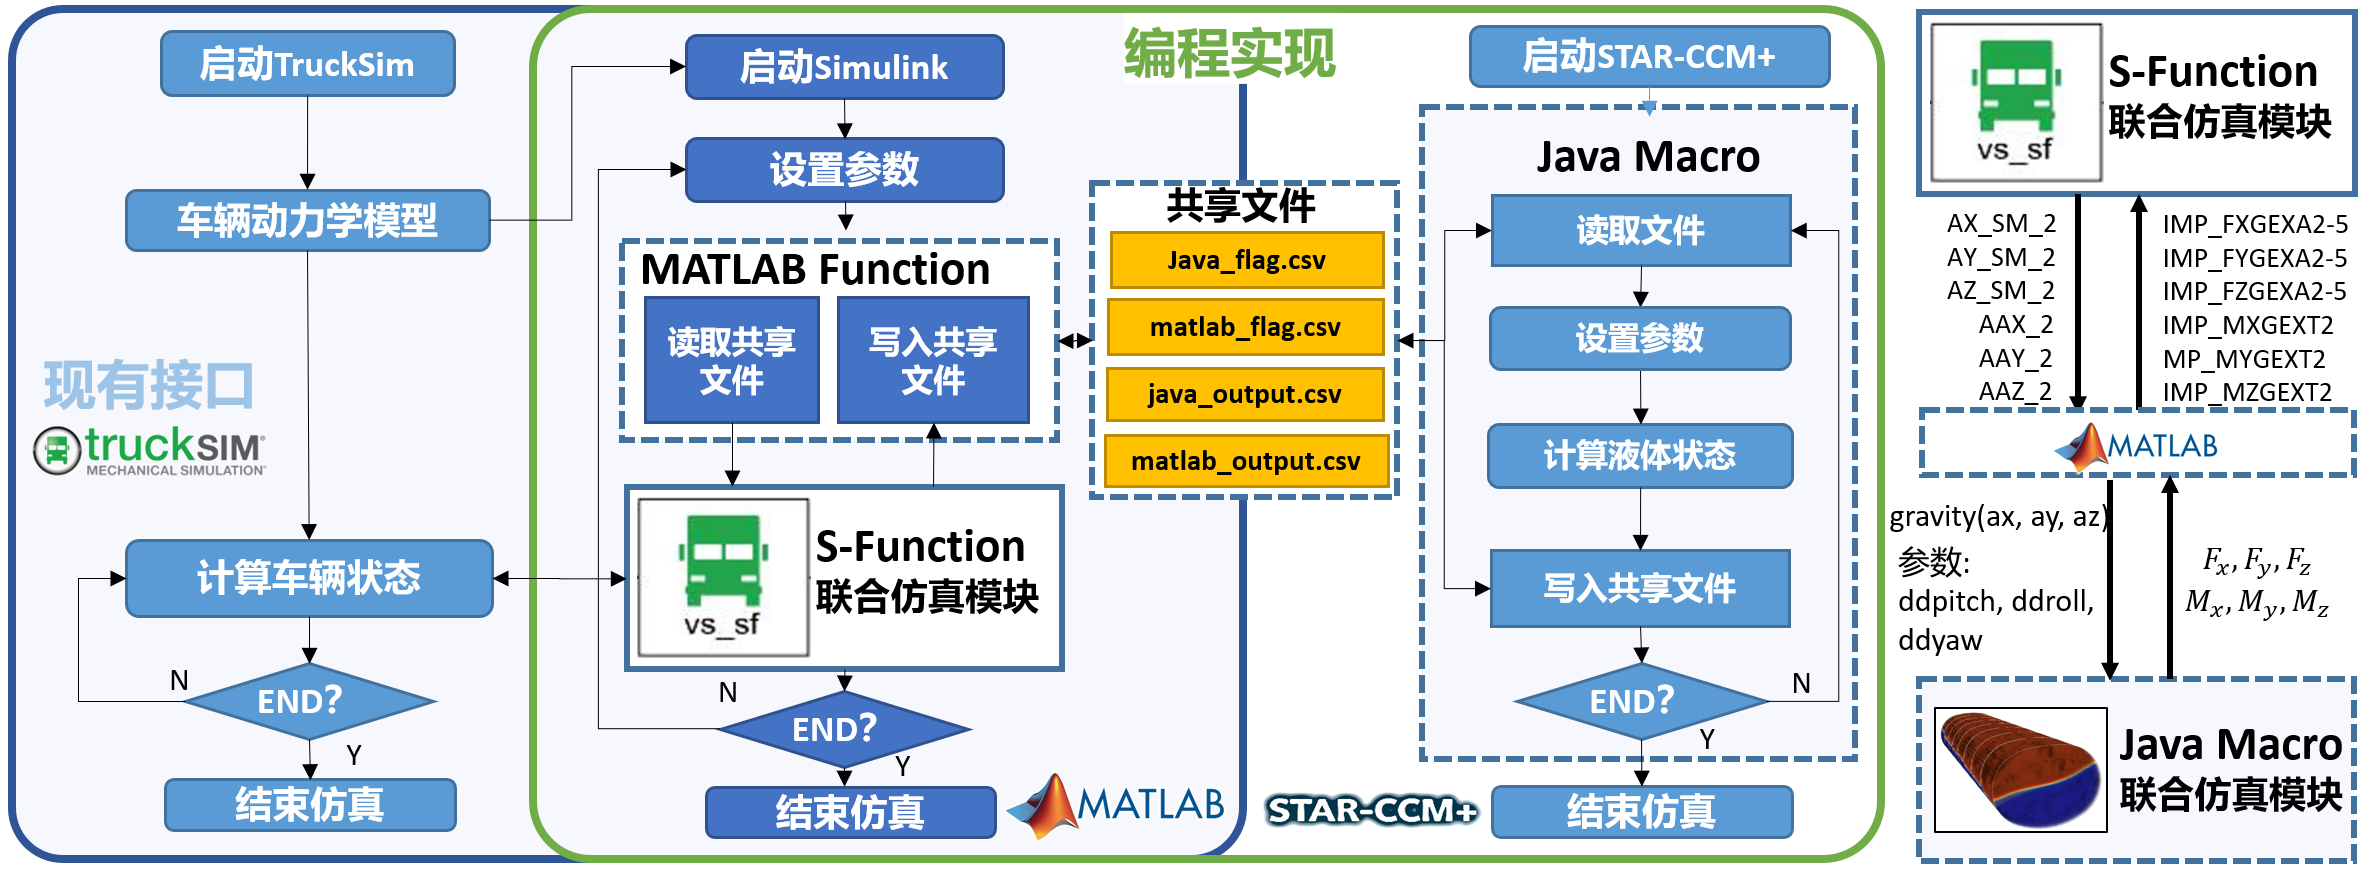
\includegraphics[width=0.94\linewidth]{fig/chap4/cosim_arch.png}}\\
  \subfloat[Grid sensitivity\label{fig:grid_sensitivity_journal}]
    {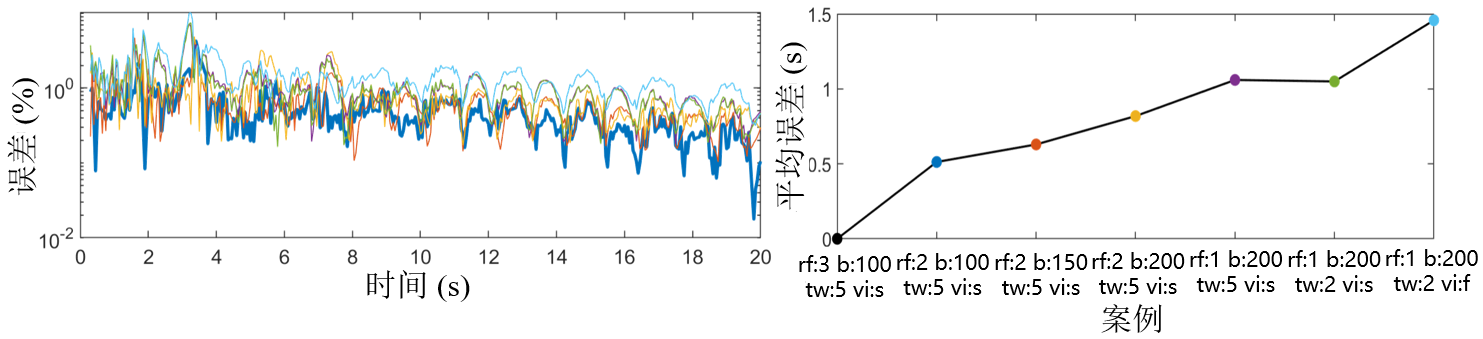
\includegraphics[width=0.94\linewidth]{fig/chap4/grid_sensitivity_res.png}}
  \caption{Vehicle-liquid co-simulation platform and CFD grid sensitivity.}
  \label{fig:cosim_validation}
\end{figure}

Four control methods were compared in the co-simulation: TruckSim preview tracking (PT), preview tracking with differential braking (PT+DB), anti-rollover tracking with steering only (ART), and the proposed anti-rollover tracking with differential braking and compensation (ART+DB). Three representative high-risk scenarios are summarized below.

In the left-turn scenario, the vehicle enters a 28.125 m left-turn radius at 35 km/h. PT rolls over at approximately 6 s. PT+DB avoids complete rollover but keeps the LTR saturated near -1 for at least 1 s. ART and ART+DB keep $\mathrm{LTR}_{eql}$ within the $\pm0.75$ soft boundary by allowing acceptable path deviation, with ART+DB producing a smaller LTR peak because differential braking assists yaw and roll stabilization.

In the SAE-J2179 single-lane-change scenario, the vehicle starts at 88 km/h and completes a 4.392 m lane change within 61 m. PT and PT+DB roll over after the lane change at around 6 s. ART sacrifices some tracking accuracy to maintain the LTR boundary. ART+DB improves tracking smoothness, uses differential braking before the risk peak, and suppresses sloshing after the maneuver.

In the short-distance double-lane-change scenario, the vehicle starts at 70 km/h, changes laterally by 3.5 m within 30 m, runs straight for 30 m, and returns within 30 m. PT already rolls over at 62 km/h in preliminary tests, confirming that the selected 70 km/h case is high risk. At 70 km/h, PT rolls over at around 6 s, PT+DB avoids complete rollover but remains near the rollover boundary for about 2.5 s, ART avoids rollover with larger tracking sacrifice, and ART+DB preserves better tracking while keeping $\mathrm{LTR}_{eql}$ within the soft boundary.

\begin{figure}[t]
  \centering
  \subfloat[Left turn\label{fig:s_corner_xu_journal}]
    {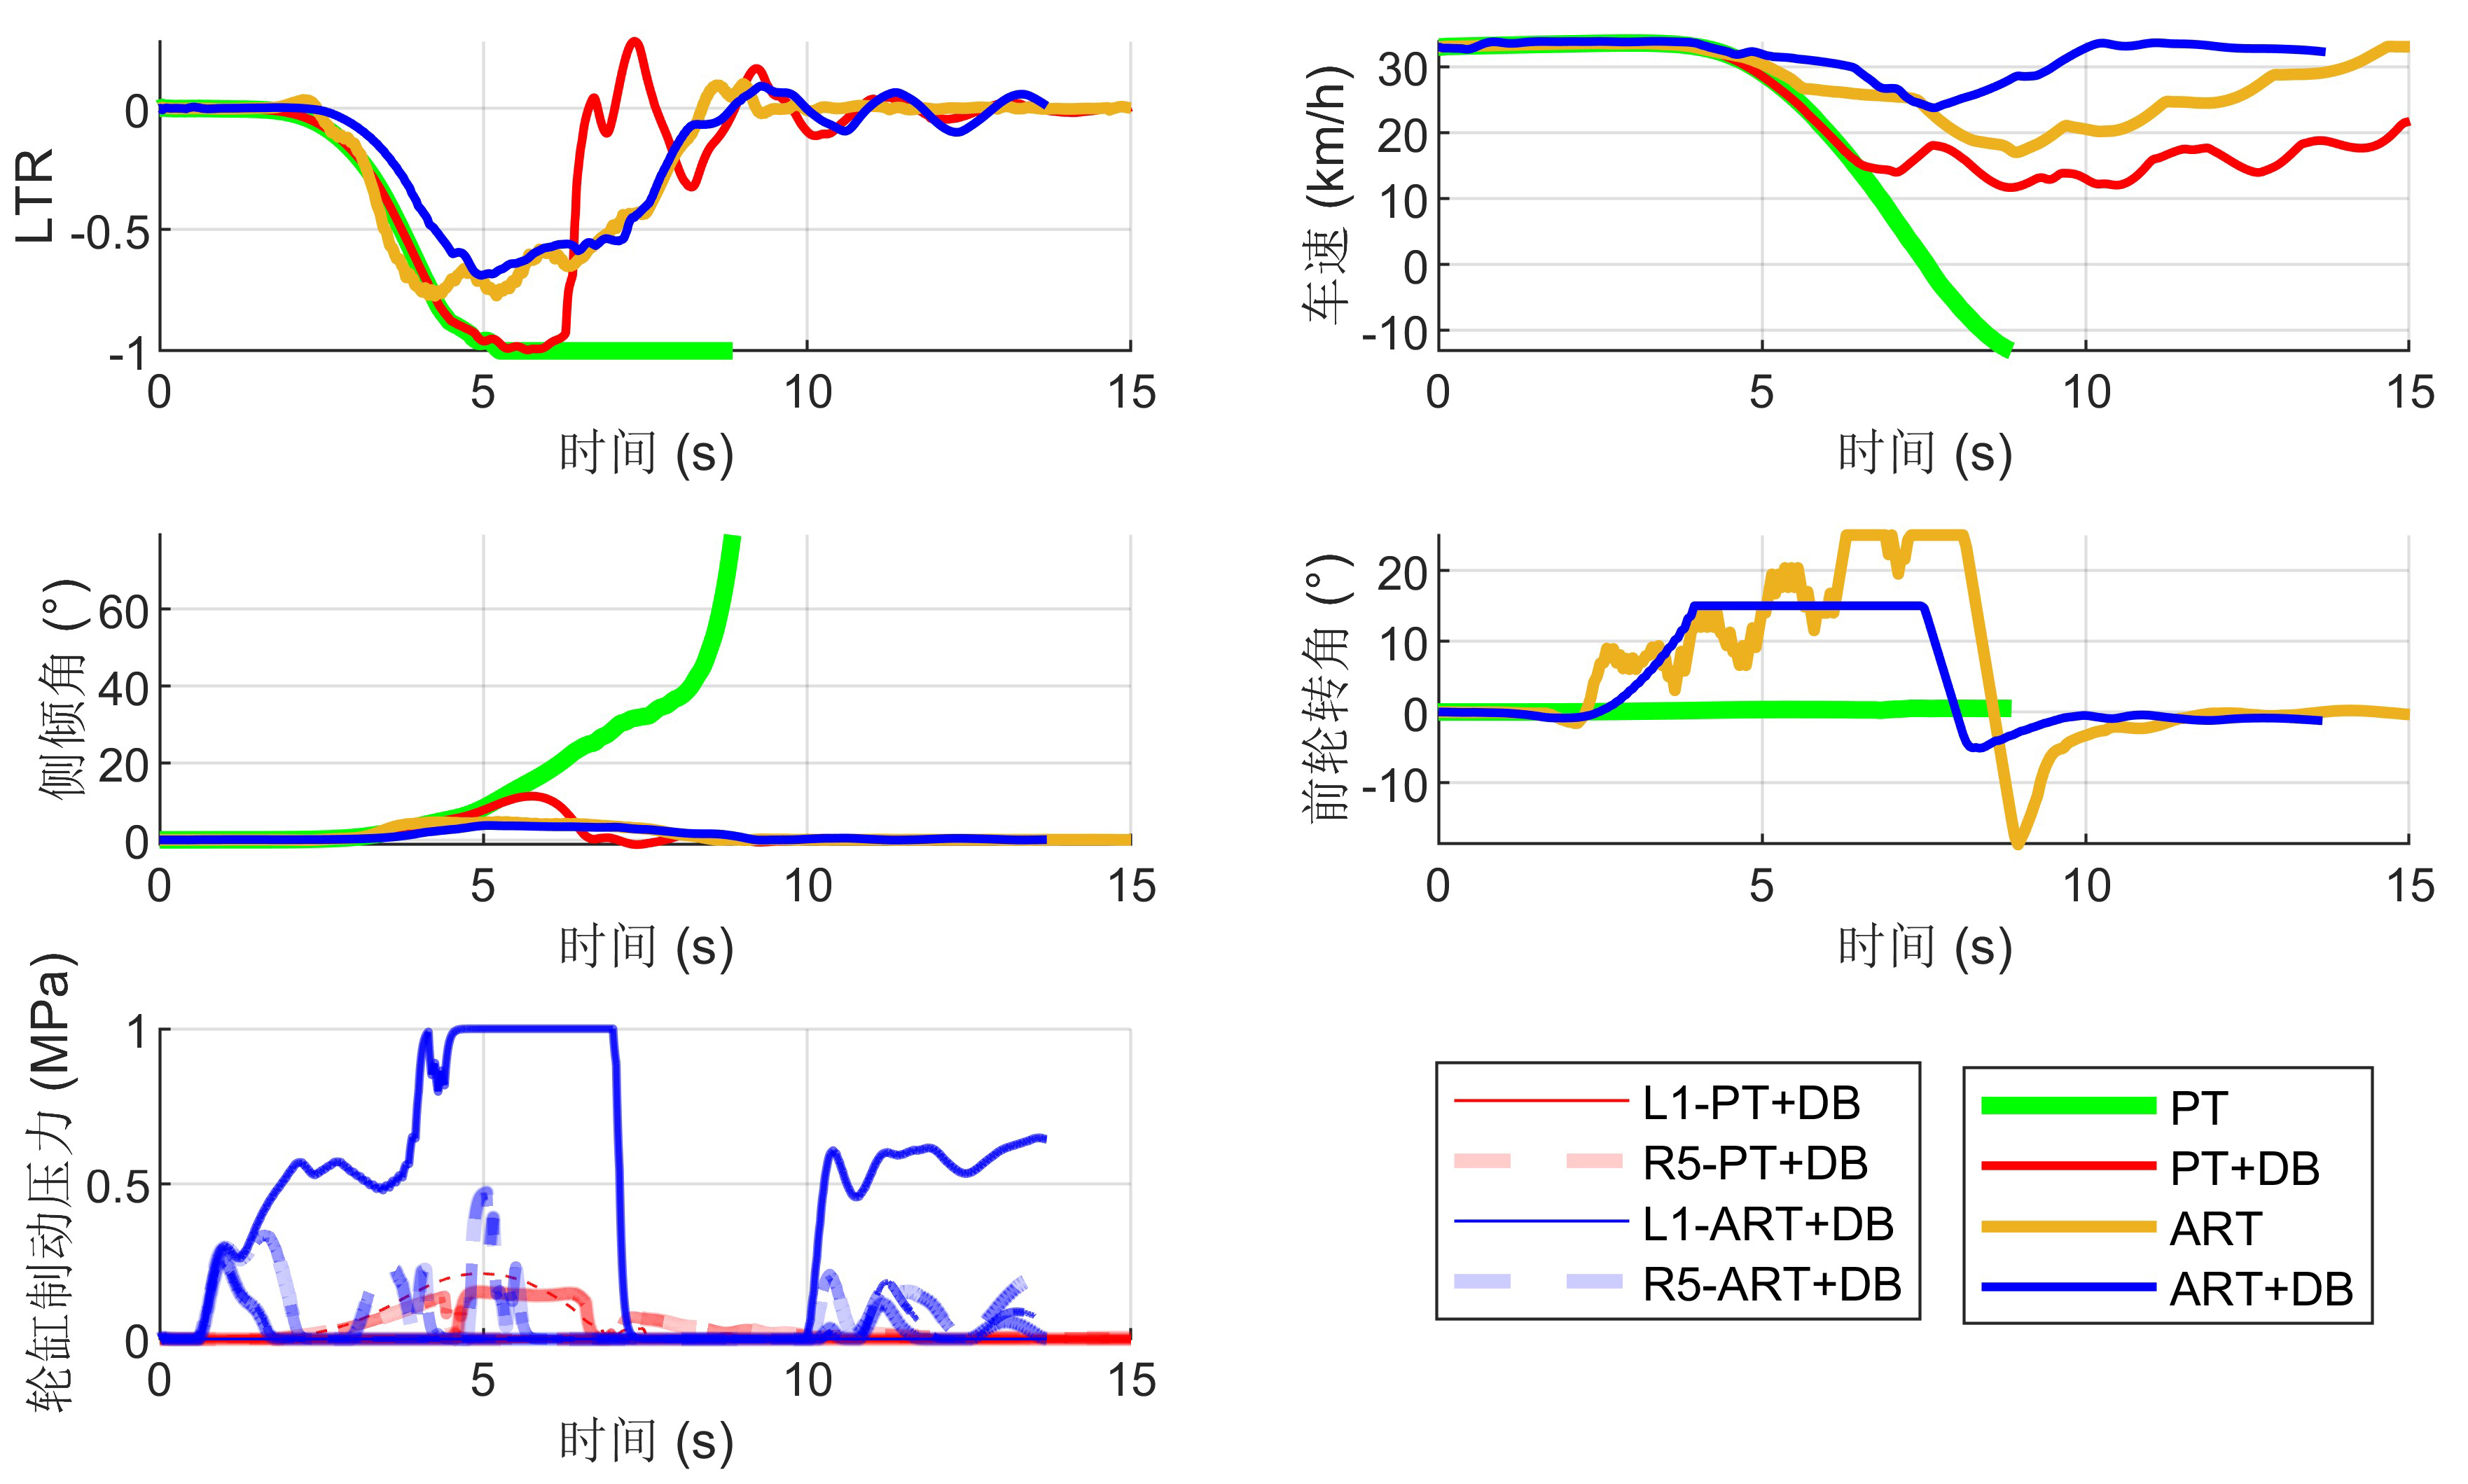
\includegraphics[width=0.95\linewidth]{fig/chap4/s_corner_xu.jpg}}\\
  \subfloat[Single lane change\label{fig:s_slc_xu_journal}]
    {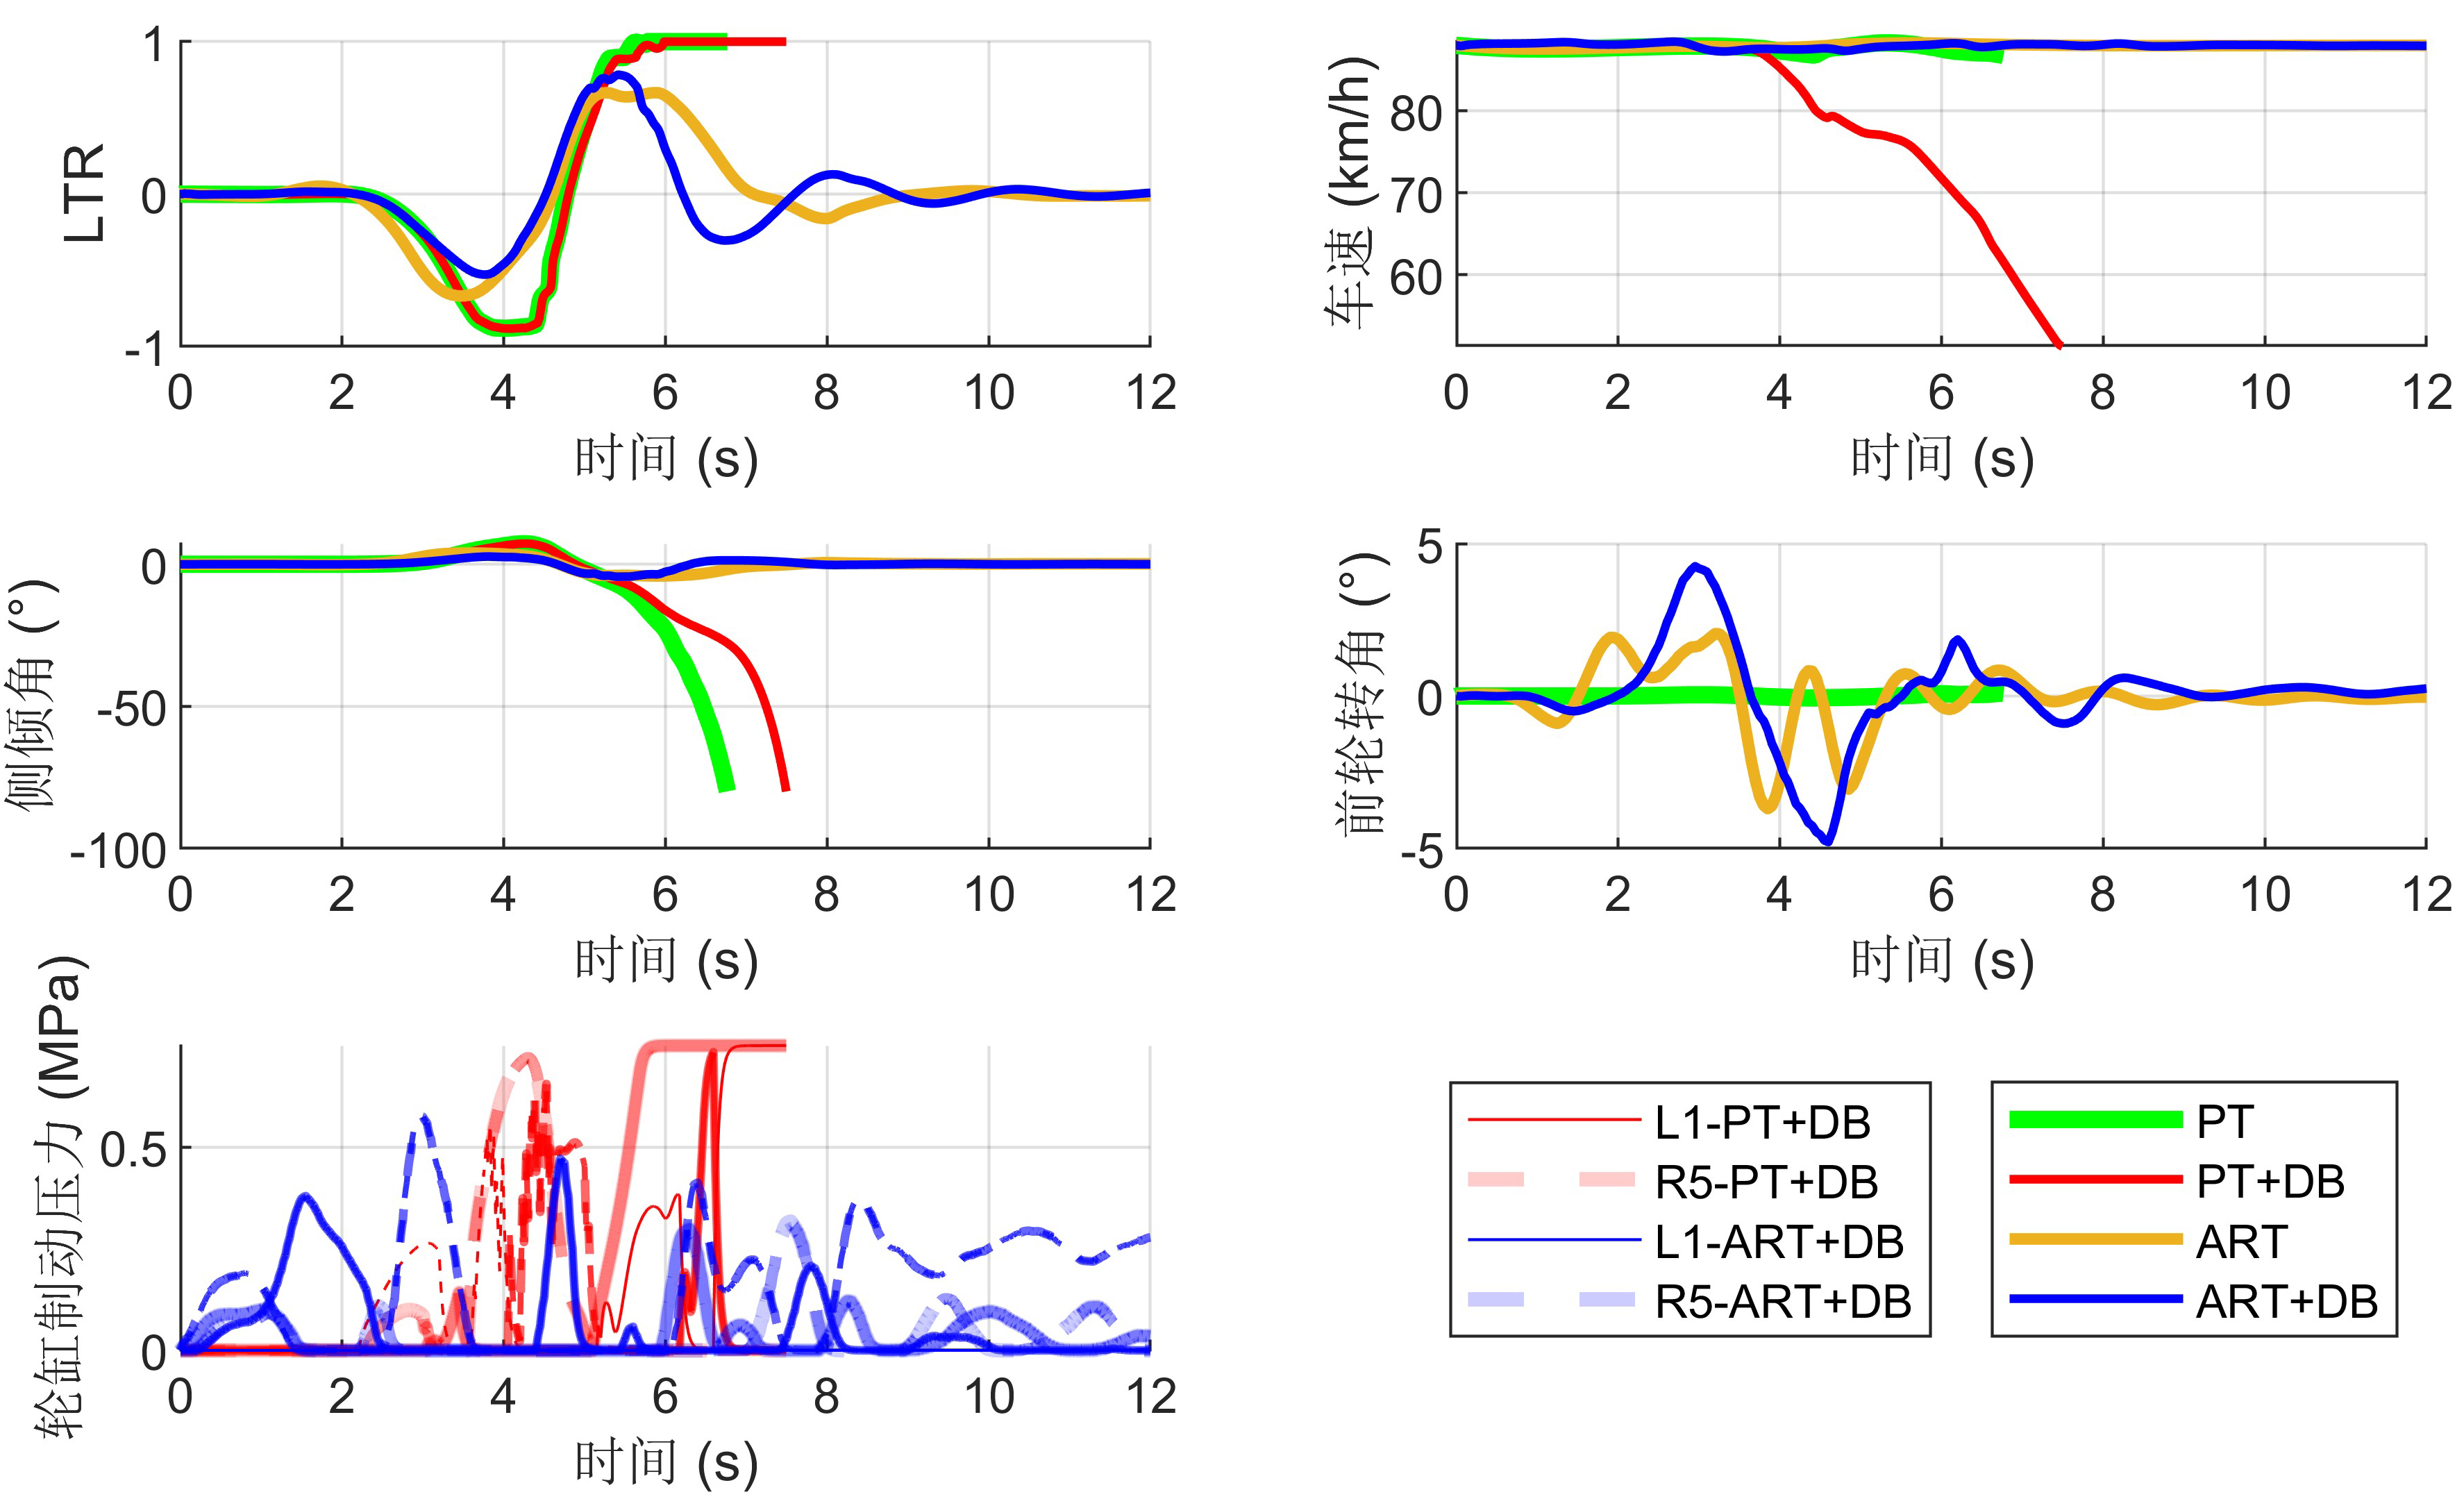
\includegraphics[width=0.95\linewidth]{fig/chap4/s_slc_xu.jpg}}\\
  \subfloat[Double lane change\label{fig:s_dlc_xu_journal}]
    {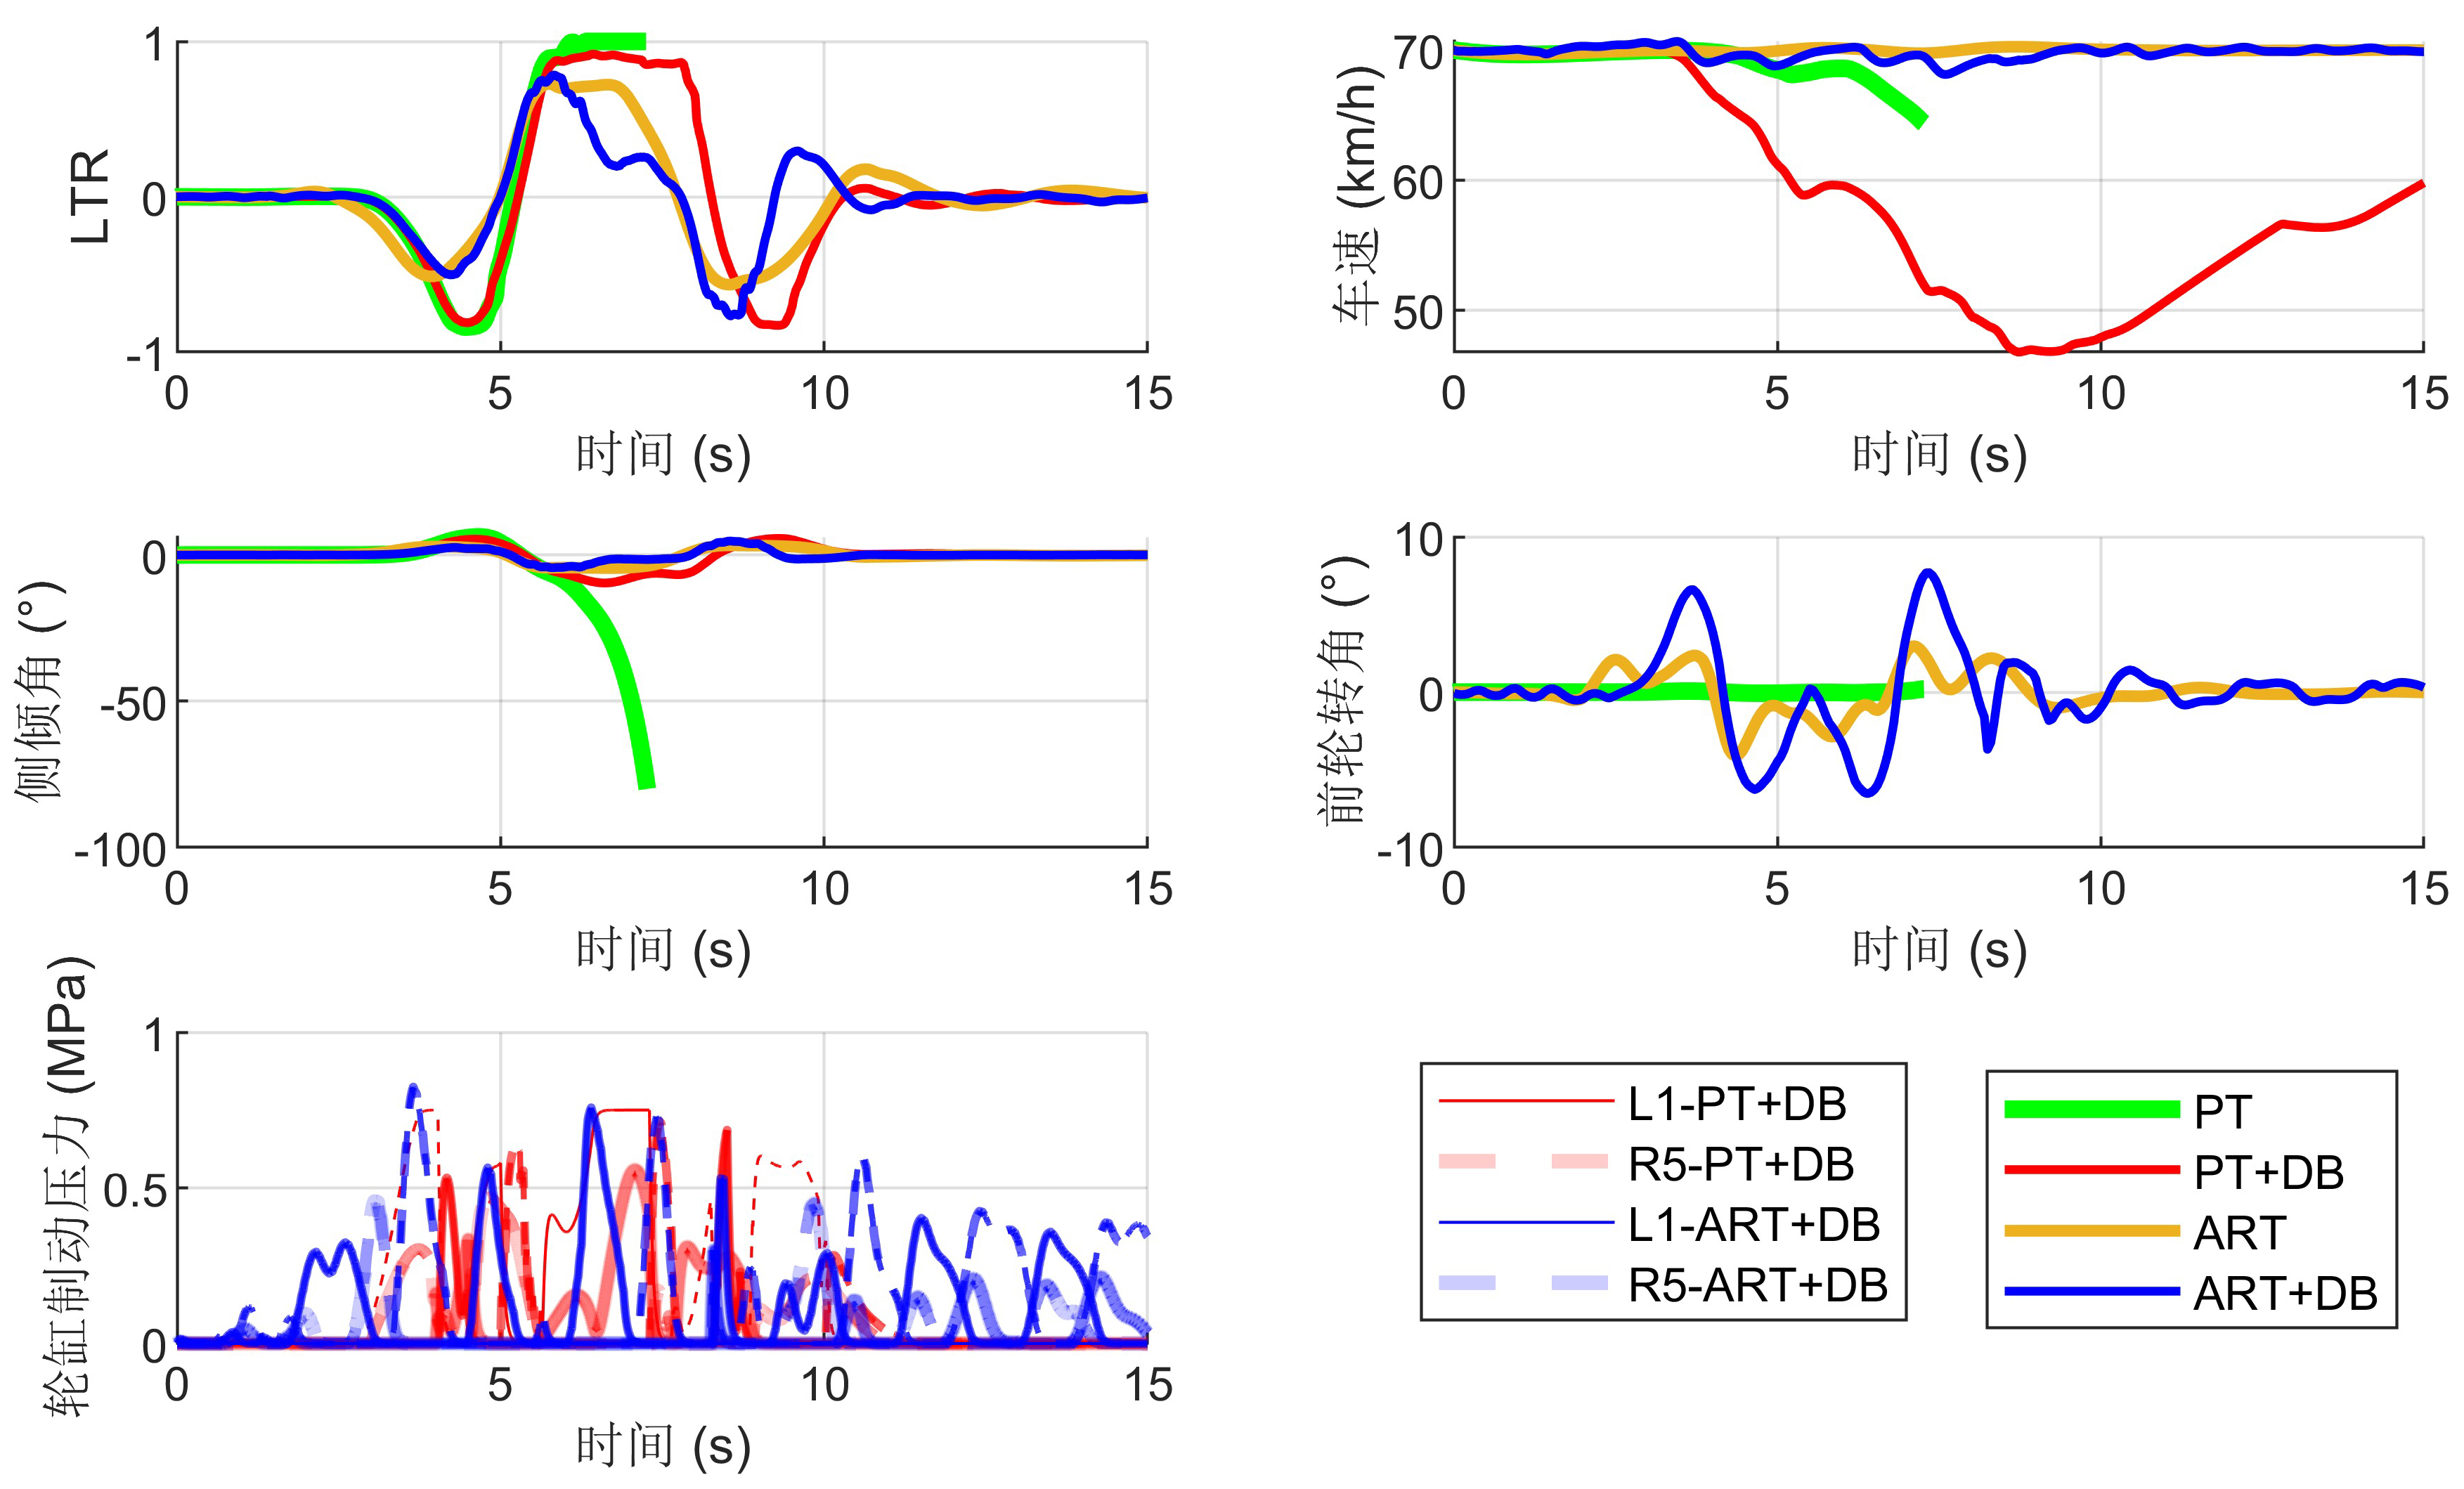
\includegraphics[width=0.95\linewidth]{fig/chap4/s_dlc_xu.jpg}}
  \caption{Vehicle-liquid co-simulation results under left-turn, SLC, and DLC scenarios.}
  \label{fig:control_cosim_results}
\end{figure}

An additional rescue test was conducted under a severe evasive maneuver. The vehicle travels at 80 km/h, the safety driver performs a sudden steering maneuver, and one-side wheel lift-off occurs at 4.7 s. PT and PT+DB continue toward rollover because they do not perform appropriate counter-steering. ART delays rollover but cannot recover without sufficient speed reduction. ART+DB combines counter-steering and strong differential braking, exits the half-rollover state, and returns toward the reference trajectory. This test indicates that the proposed controller extends the recoverable domain beyond ordinary LTR-constrained tracking cases.

\subsection{Scaled Tank-Truck Experimental Validation}

A 1:14 scaled semi-trailer tank-truck platform was built for experimental validation. The model has a total length of 1250 mm after tank installation, a width of 200 mm, a height of 350 mm, a mass of 42 kg, and a maximum speed of about 3 m/s. The platform includes IMU/GNSS units, wheel encoders, perception sensors, a Jetson Orin NX controller, and an acrylic liquid tank with anti-surge plates. Similarity analysis was used to relate the scaled test to prototype lateral acceleration and liquid-sloshing time scale. For free-surface sloshing, the Froude number and the sloshing-period relation were used to design the double-lane-change test trajectory.

\begin{figure}[t]
  \centering
  \subfloat[Hardware platform\label{fig:hardware_journal}]
    {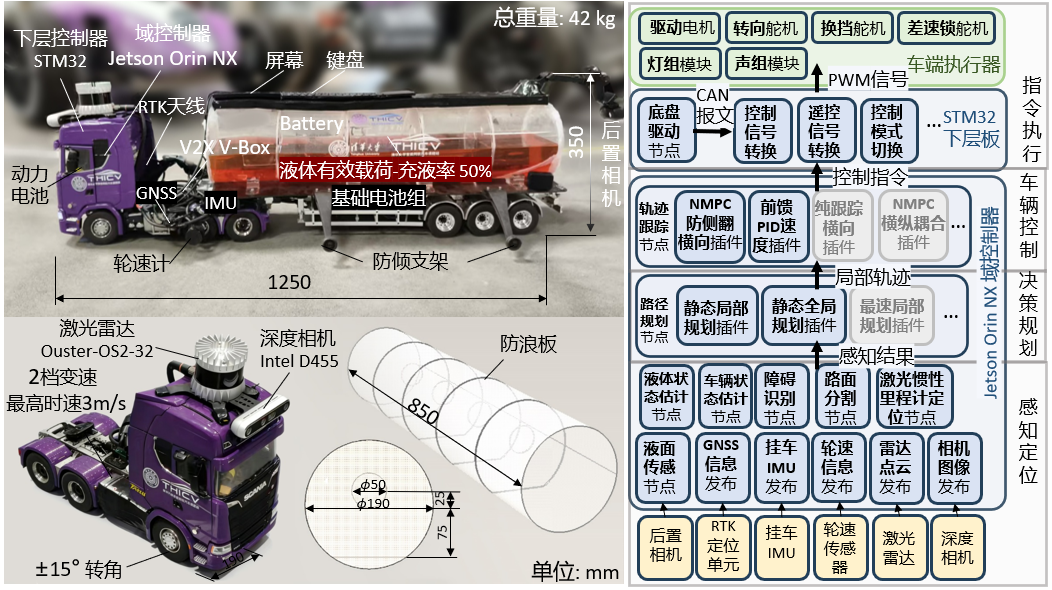
\includegraphics[width=0.95\linewidth]{fig/chap4/hardware.png}}\\
  \subfloat[Similarity and reference design\label{fig:exp_ref_pic_journal}]
    {\includegraphics[width=0.95\linewidth]{fig/chap4/exp_ref_traj.jpg}}
  \caption{Scaled tank-truck experimental platform and reference trajectory design.}
  \label{fig:scaled_platform}
\end{figure}

The experiment compares pure tracking and anti-rollover control. The controller runs at 20 Hz with prediction horizon $N_p=15$, control horizon $N_c=5$, and constrained horizon $N_r=5$. In low-speed slalom, both methods maintain small tracking errors. In the high-speed short-distance double-lane-change test, both vehicles maintain approximately 2.5 m/s, but the pure-tracking case produces severe sloshing and touches the anti-rollover support during 3--3.5 s and 4--4.5 s of the maneuver. This support contact corresponds to rollover in a full-scale unprotected vehicle.

The anti-rollover controller delays the return to the original lane and keeps the LTR inside the soft boundary. The trailer roll angle remains within about $\pm5\degree$, and the liquid free-surface angle remains approximately within $[-15\degree,15\degree]$. In contrast, the pure-tracking method reaches about 6--7 degrees trailer roll during the two lane-change peaks, the LTR reaches 1 around 3 s and 4.5 s, and the liquid angle exceeds 20 degrees multiple times. The maximum roll-angle reduction of the anti-rollover controller is about 42\%. The average solver time is 15.4 ms, and the peak solver time is below 25 ms.

\begin{figure}[t]
  \centering
  \subfloat[Experiment photographs\label{fig:cond_pic_journal}]
    {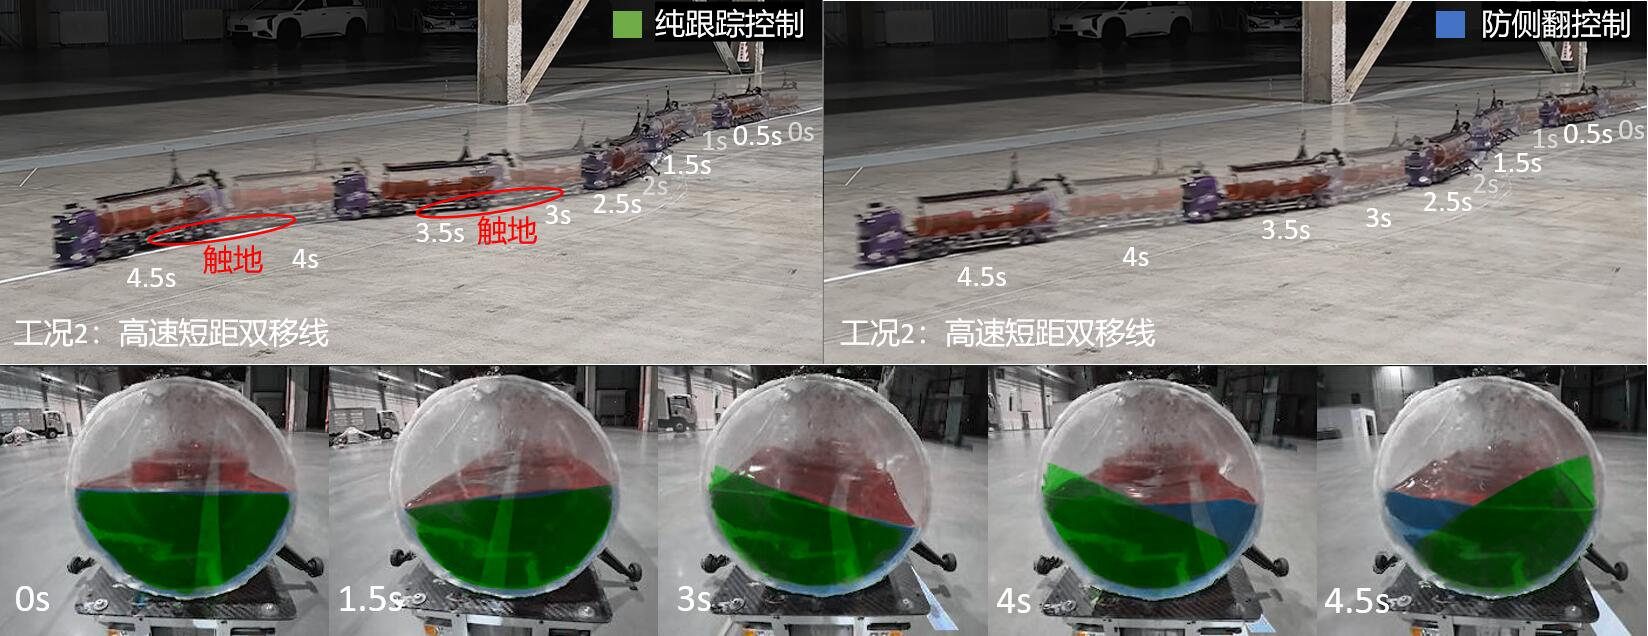
\includegraphics[width=0.95\linewidth]{fig/chap4/cond2_pic.jpg}}\\
  \subfloat[Trajectory tracking\label{fig:exp_traj_journal}]
    {\includegraphics[width=0.95\linewidth]{fig/chap4/exp_traj.jpg}}\\
  \subfloat[Vehicle states\label{fig:exp_x_journal}]
    {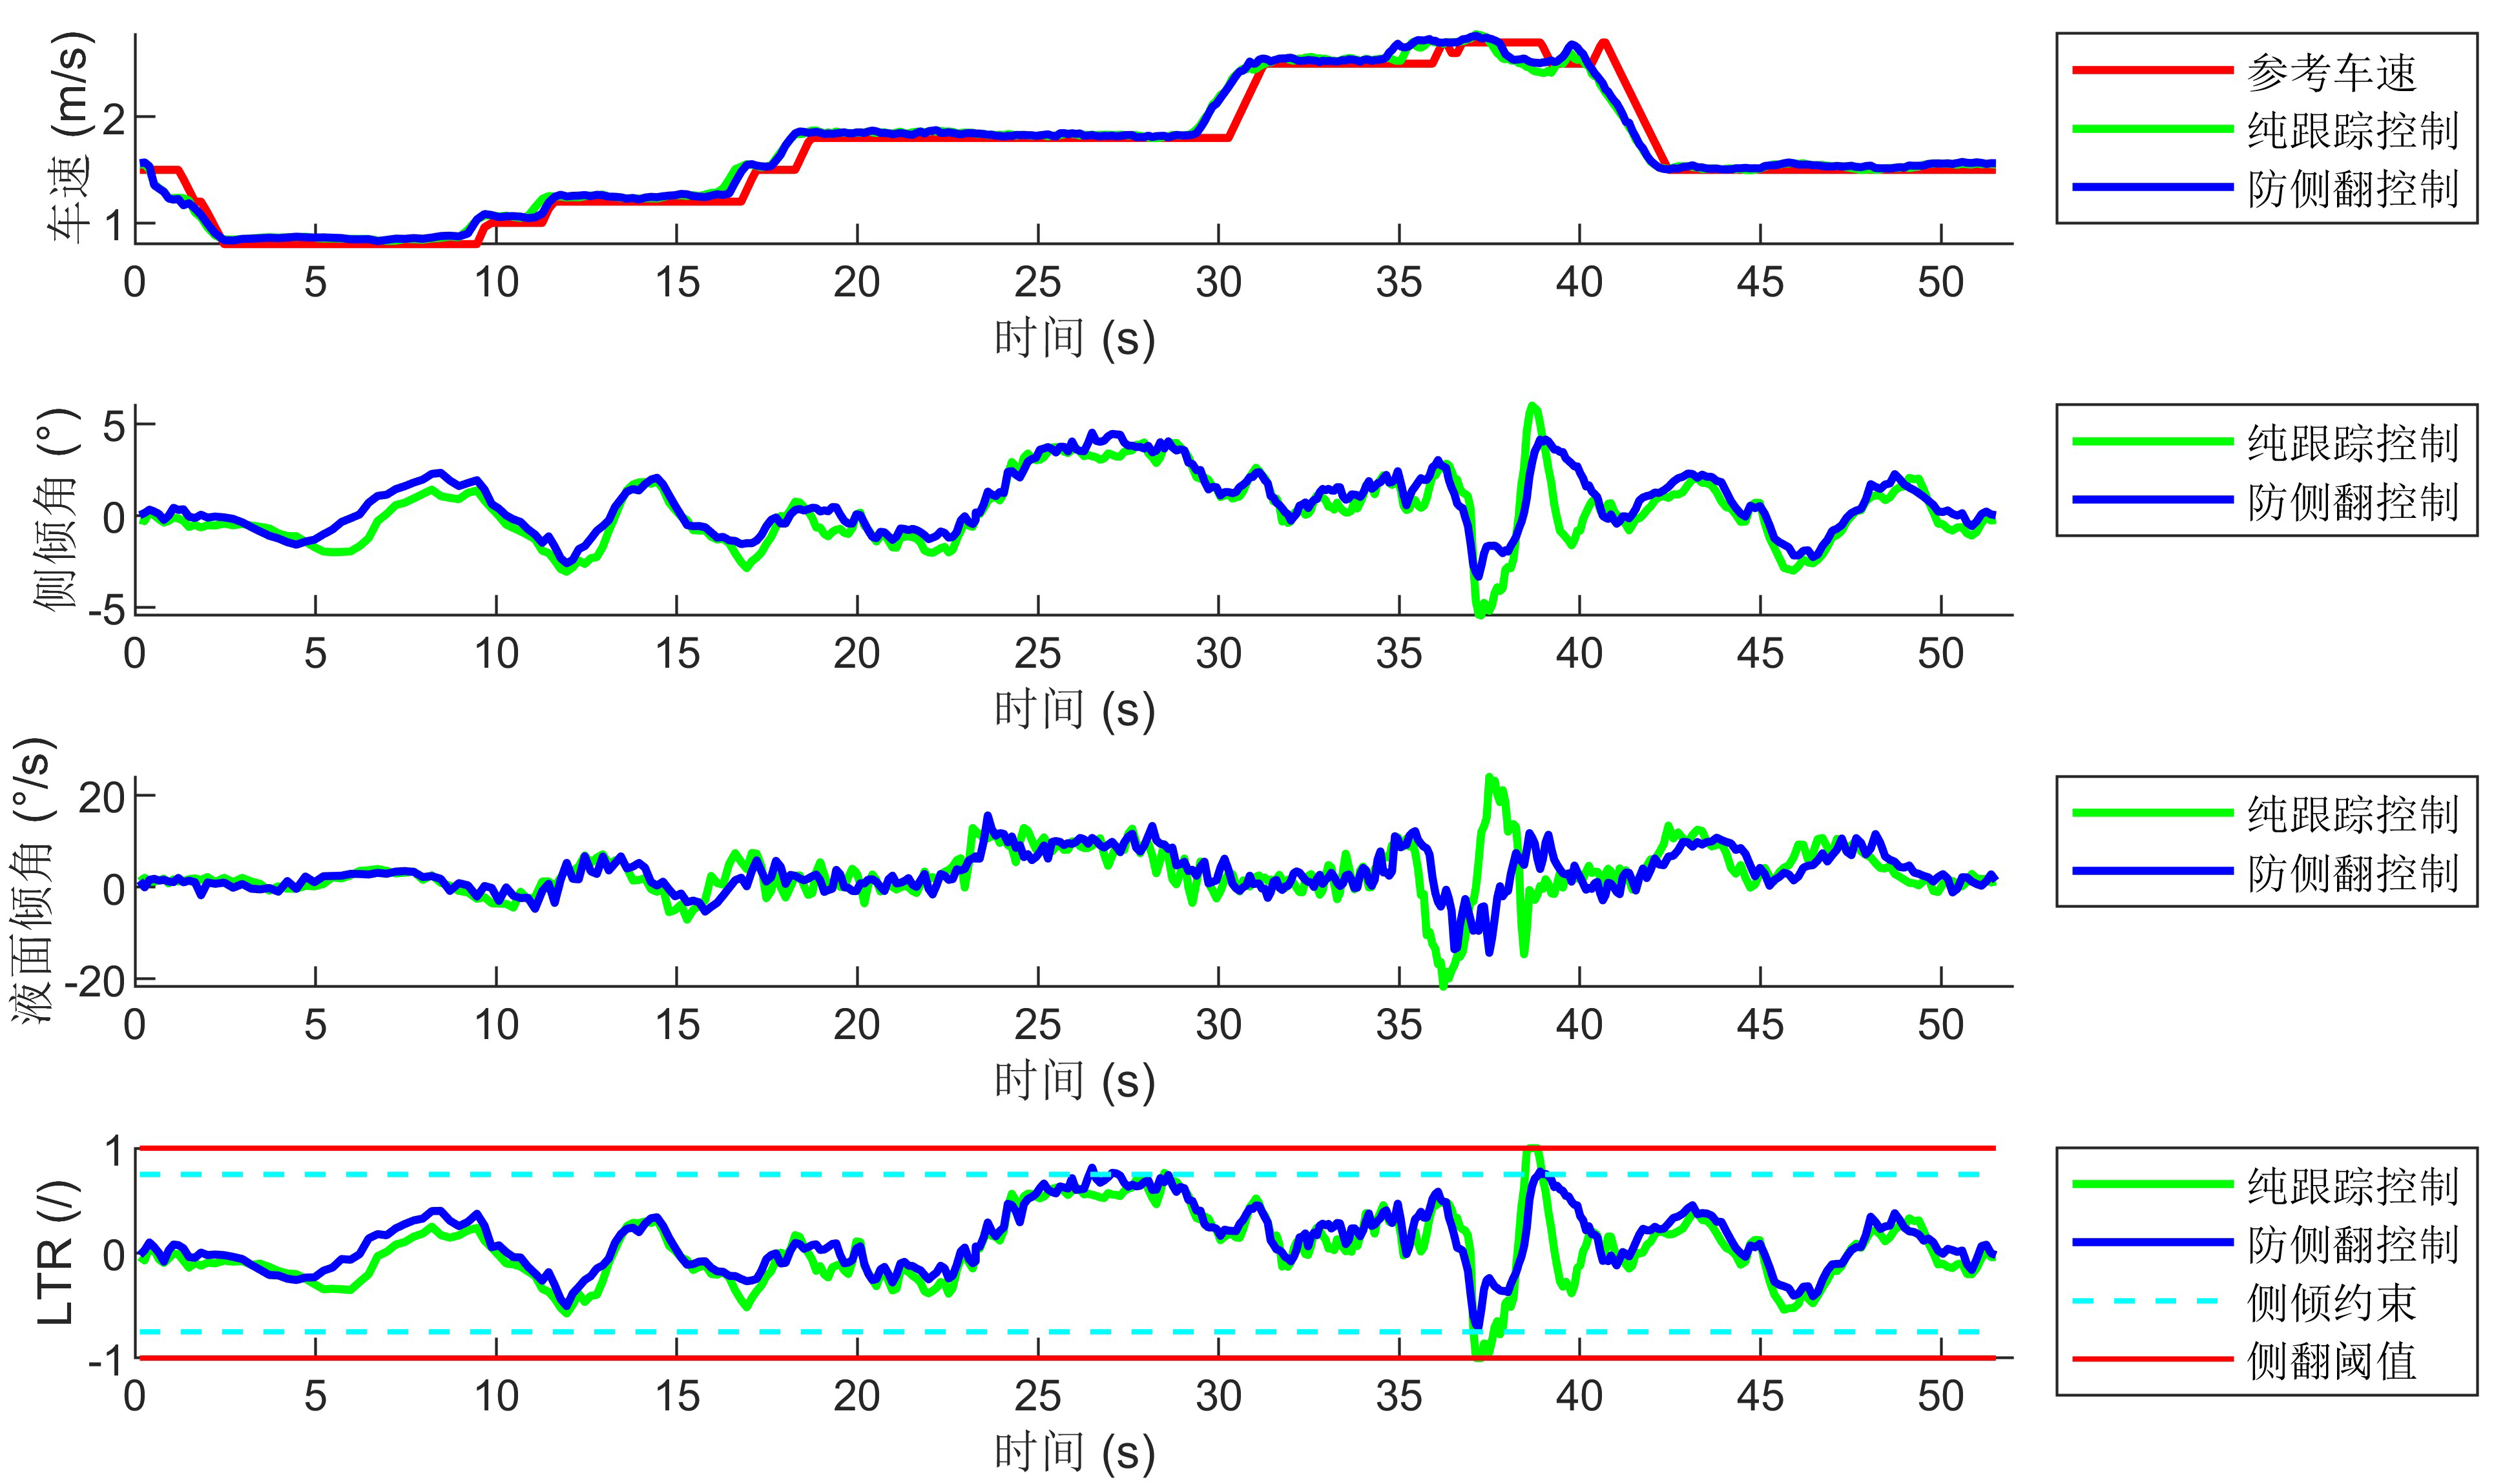
\includegraphics[width=0.95\linewidth]{fig/chap4/exp_x.jpg}}\\
  \subfloat[Control and solver time\label{fig:slack_iter_journal}]
    {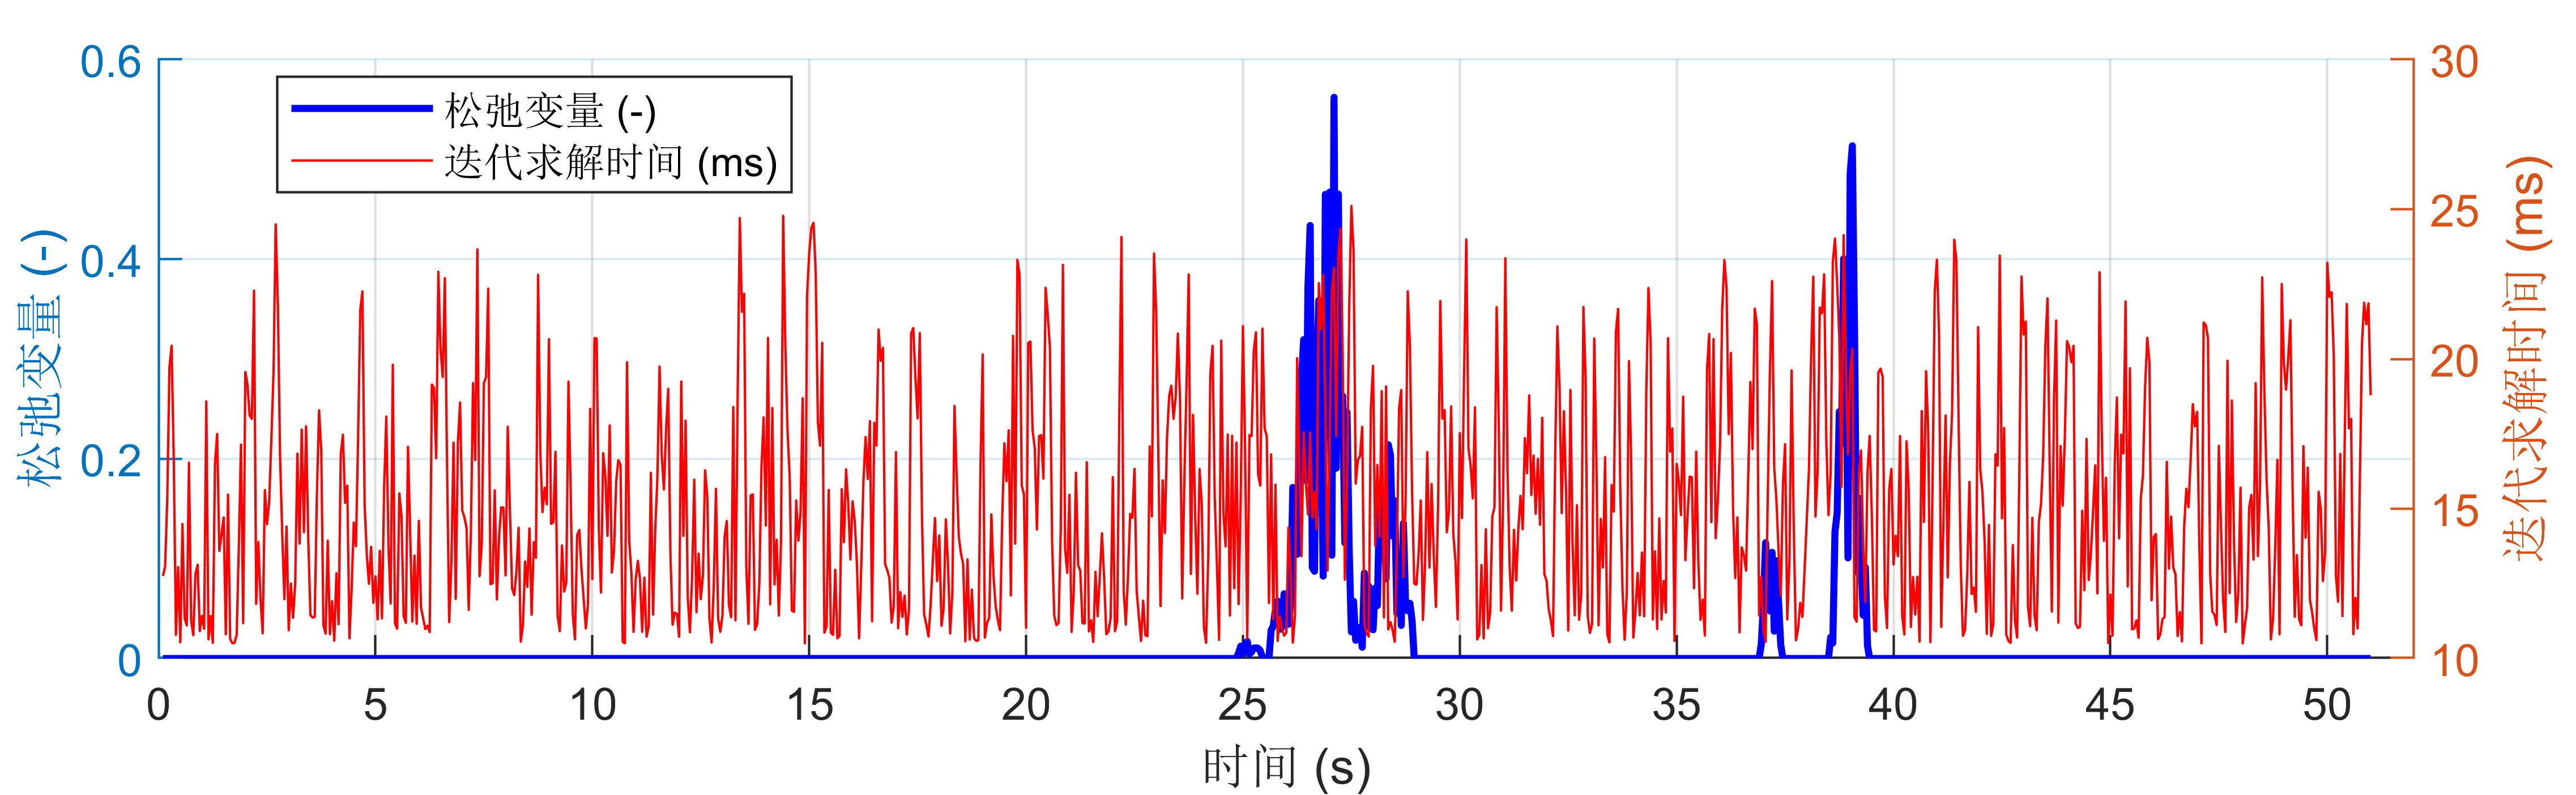
\includegraphics[width=0.95\linewidth]{fig/chap4/slack_iter.jpg}}
  \caption{Scaled model-truck experimental validation.}
  \label{fig:model_experiment_results}
\end{figure}

\subsection{Ablation and Real-Time Analysis}

The available validation supports the role of each major layer. Removing long-horizon prediction reduces the system to the single-vehicle IDM+MOBIL baseline, which is consistently less safe in the traffic validation set. Removing rollover-aware execution reduces the system to PT or PT+DB, which fails or approaches the rollover boundary in the high-risk co-simulation cases. Removing the coupled steering-braking MPC compensation reduces the system to ART, which can prevent rollover but sacrifices more tracking performance and has less recovery capability in the rescue case. Table~\ref{tab:ablation_plan} summarizes the ablation evidence currently available from the thesis.

\begin{table*}[t]
  \centering
  \caption{Ablation Evidence Available in the Current Draft}
  \label{tab:ablation_plan}
  \begin{tabularx}{0.96\textwidth}{p{0.24\textwidth}p{0.35\textwidth}X}
    \toprule
    Removed module & Available comparison & Main observation \\
    \midrule
    Cloud-side prediction and RL decision & IDM+MOBIL vs. Graphflow policy in 280 validation runs & Predictive planning improves safety-related scores while keeping efficiency comparable. \\
    Rollover-aware reference and control & PT vs. ART/ART+DB in left-turn, SLC, and DLC co-simulation & Pure tracking rolls over in multiple high-risk scenarios. \\
    Differential braking and compensation in MPC & ART vs. ART+DB in co-simulation & ART+DB improves tracking and recovery while keeping LTR within the soft boundary. \\
    Anti-rollover MPC in scaled tests & Pure tracking vs. anti-rollover control & Anti-rollover control reduces maximum roll angle by 42\% and avoids support contact. \\
    \bottomrule
  \end{tabularx}
\end{table*}
% TODO: Complete a numerical ablation table after extracting uniform metrics from the simulation logs: maximum tracking error, maximum LTR, maximum roll angle, sloshing amplitude, collision/conflict rate, and solver time for each module combination.

Real-time feasibility is supported at two levels. On the cloud side, Graphflow and PPO are trained offline; online inference provides low-frequency predictive guidance. The reported training times are 6.9 h for Graphflow and 8.3 h for the PPO decision model on a single RTX 5070 Laptop GPU. On the vehicle side, the scaled platform demonstrates 20 Hz MPC execution with an average solution time below the 50 ms control period. Full cloud-edge deployment tests with communication delay and packet loss remain future work.


\section{Conclusion}

This paper presented a vehicle-cloud collaborative predictive planning and anti-rollover control framework for autonomous tank trucks. The framework follows a nested safety logic: the cloud-side outer loop anticipates interaction-induced risks through Graphflow-based prediction and reinforcement-learning decision-making, the vehicle-side planning loop provides contingency fallback when the cloud reference becomes locally unsafe, and the high-frequency control loop suppresses roll and liquid-sloshing state risks through multi-constraint MPC. In this structure, the cloud trajectory is predictive guidance rather than a direct command, and the vehicle remains responsible for real-time feasibility and anti-rollover safety.

Validation was conducted through traffic simulation, vehicle-liquid co-simulation, and scaled tank-truck experiments. In the G15 highway traffic simulation, Graphflow provided long-horizon risk-field prediction and the cloud-side policy improved safety-related scores over a single-vehicle baseline while maintaining comparable efficiency. The vehicle-side planner generated feasible contingency behaviors in representative local conflict cases. In co-simulation, the proposed steering-braking MPC kept the equivalent LTR within the soft safety boundary in high-risk left-turn, single-lane-change, and double-lane-change scenarios where pure tracking or late differential braking failed or approached rollover. In scaled experiments, the controller reduced the maximum roll angle by 42\% and achieved real-time execution with an average solution time of 15.4 ms.

Several limitations remain. Full-scale real-vehicle validation has not yet been conducted, and the influence of communication delay, packet loss, and cloud-edge deployment constraints should be studied in closed-loop experiments. The current traffic validation focuses on highway and interchange scenarios; more complex mixed-traffic, ramp, construction-zone, and adverse-weather cases should be added. Future work will also improve quantitative ablation coverage and investigate deployment-efficient cloud-edge implementations for real hazardous-liquid transportation systems.


% \section*{Acknowledgments}
% This should be a simple paragraph before the References to thank those individuals and institutions who have supported your work on this article.

\appendices

\section{Architecture Modeling Details}

The main text only uses the architecture analysis to define system boundaries and time scales. The original architecture study follows a scenario-oriented model and simulation based system-of-systems engineering process. It treats vehicle-cloud collaborative tank-truck rollover prevention as a low-penetration highway mission in an intelligent vehicle cyber-physical system. The full architecture contains strategic, operational, service, and resource views. These views are useful for tracing requirements, but they are not necessary for the main algorithmic derivation.

The resulting design constraints used in this paper are as follows. First, the cloud side is an advisory and predictive layer rather than a direct actuator controller, and its main safety role is to reduce induced interaction risks before the ego vehicle enters a local emergency. Second, the vehicle side must maintain an independent safety loop because the cloud message may be delayed, lost, or invalidated by local perception. Third, the layered periods are approximately 1--2 Hz for cloud-side predictive planning, 10 Hz for vehicle-side emergency planning, and 20 Hz or higher for high-frequency anti-rollover control. Fourth, the emergency response chain must remain vehicle-side executable even when the cloud service is unavailable, so degraded safety does not rely on cloud availability.

\begin{figure}[t]
  \centering
  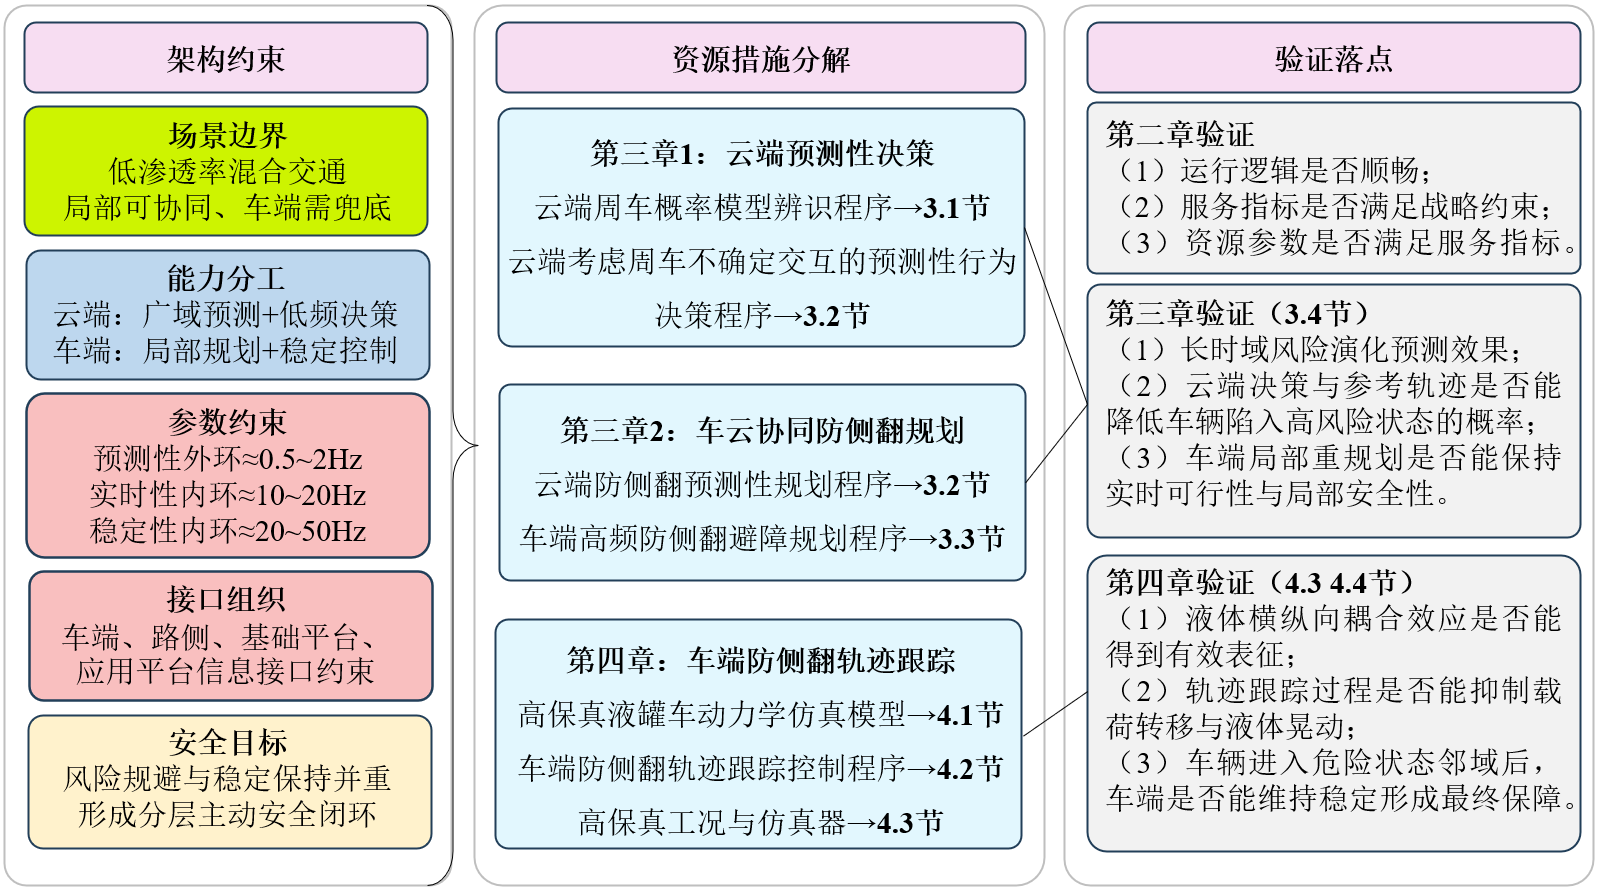
\includegraphics[width=0.95\linewidth]{fig/chap2/arch_method_mapping_v3.png}
  \caption{Traceability from architecture constraints to cloud-side planning, vehicle-side planning, and vehicle-side anti-rollover control.}
  \label{fig:appendix_arch_trace}
\end{figure}
% TODO: Redraw this appendix figure in English if the architecture traceability result is retained in the submitted manuscript.

\section{Graphflow Training and Decision Policy Details}

The Graphflow dataset is constructed by extracting a fixed road-graph region around the ego vehicle. The source implementation uses a forward range of about 700 m and a backward range of about 300 m to cover long-horizon highway interactions. Historical and future dynamic node features are mapped to the same graph topology, so autoregressive prediction can be performed by updating node features while keeping the edge set fixed.

The graph encoder uses three information sources: node features, edge features, and conditioning features. Node features describe static road semantics and dynamic traffic occupancy. Edge features describe road connectivity and lane-changing relations. Conditioning features include time encoding and ego action encoding. Local graph attention aggregates edge-aware neighbor information, while global attention captures long-range interaction over the graph. The output head predicts the dynamic-feature velocity field used in the flow-matching objective.

The reinforcement-learning decision policy uses a shared feature extractor for actor and critic. It encodes the traffic graph, ego features, and surrounding-vehicle historical features, then outputs an action sequence consisting of desired acceleration and lane-change command. The reward terms used in training are summarized in Table~\ref{tab:appendix_reward}.

\begin{table}[t]
  \centering
  \caption{Cloud-Side Policy Reward Terms}
  \label{tab:appendix_reward}
  \begin{tabularx}{\linewidth}{p{0.22\linewidth}X}
    \toprule
    Term & Role \\
    \midrule
    Safety & Penalizes ego occupancy on high graph-risk fields over the prediction horizon. \\
    Efficiency & Rewards speed close to road speed limits. \\
    Comfort & Penalizes acceleration magnitude and unnecessary lane changes. \\
    Consistency & Penalizes discontinuity between successive planned action sequences. \\
    Rule compliance & Penalizes speeding and unnecessary left-lane occupation. \\
    Navigation & Rewards staying on route-consistent graph nodes. \\
    \bottomrule
  \end{tabularx}
\end{table}

\section{Liquid-Sloshing Model Details}

The high-fidelity rapid sloshing model used in the thesis is the sliding telescopic libra model. It represents longitudinal-lateral coupled liquid motion through sliding lumped masses on smooth surfaces and curves. Compared with a two-dimensional pendulum model, this structure can describe liquid mass transfer between tank chambers, additional yaw moment induced by tank rotation, and longitudinal-lateral coupling under simultaneous acceleration, roll, and yaw excitation. The model was introduced to preserve the key six-degree-of-freedom sloshing modes needed by anti-rollover control while remaining much faster than CFD during repeated prediction.

The STL model can be written as
\begin{equation}
  [X_{STL}(k+1),Q_{STL}(k+1)]
  =f_{STL}(X_{STL}(k),u_l(k)|w_{STL}),
  \label{eq:appendix_stl}
\end{equation}
where $X_{STL}$ is the liquid-equivalent state, $u_l=[a_x,a_y,\phi,\ddot{\phi},\dot{\psi},\ddot{\psi}]^T$ is the tank excitation input, $w_{STL}$ is the identified parameter vector, and $Q_{STL}$ contains the equivalent liquid forces and moments. Parameters are identified from CFD data by minimizing the force/moment error over orthogonal excitation cases.

\begin{figure}[t]
  \centering
  \subfloat[STL model construction\label{fig:appendix_stl_model}]
    {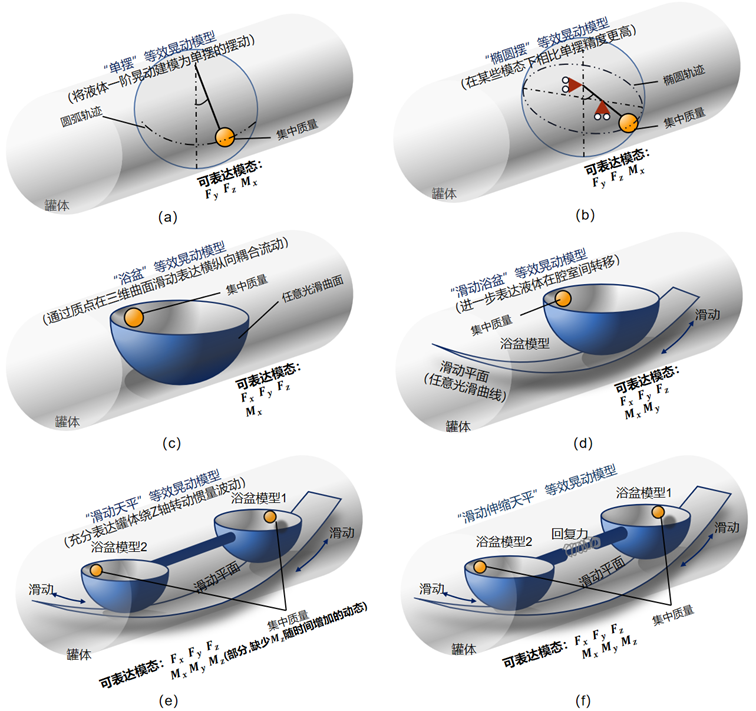
\includegraphics[width=0.95\linewidth]{fig/chap4/stl_model.png}}\\
  \subfloat[Residual re-linearization\label{fig:appendix_residual_learning}]
    {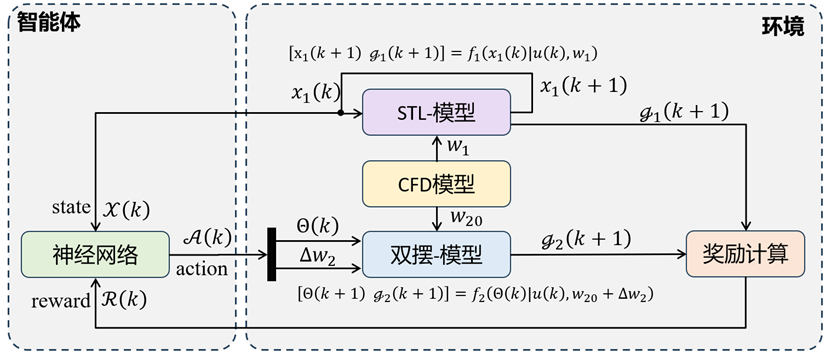
\includegraphics[width=0.95\linewidth]{fig/chap4/residual_learning.png}}
  \caption{Liquid-sloshing modeling and residual re-linearization.}
  \label{fig:appendix_liquid_model}
\end{figure}

For online MPC, the STL model is converted into a linearized double-pendulum model. A residual reinforcement-learning model maps the current STL state to parameter corrections and state estimates for the LDP model:
\begin{equation}
  [\Theta,\Delta w_{LDP}]=n_{\varphi}(X_{STL}),
  \label{eq:appendix_residual}
\end{equation}
where $\Theta$ is the LDP state estimate and $\Delta w_{LDP}$ is the parameter correction. The training reward penalizes the multi-step force/moment mismatch between STL and LDP outputs over representative excitations.

\section{Additional Validation and Platform Details}

The vehicle-liquid co-simulation platform couples TruckSim, Simulink, and StarCCM+. TruckSim provides vehicle acceleration and angular motion to the CFD model. StarCCM+ returns liquid forces and moments to the vehicle model. The data exchange interval in the reported co-simulation is 0.005 s. The liquid phase is gasoline-like $C_8H_{17}$ with 50\% filling ratio. The selected mesh setting is obtained from grid sensitivity analysis with average relative error below 1\% and peak error below 4\%.

The scaled experimental platform is a 1:14 semi-trailer model with an acrylic tank and anti-surge plates. The controller is implemented in C++ under ROS on a Jetson Orin NX. State measurements include IMU/GNSS pose and angular motion, wheel-encoder speed, and estimated liquid states. The similarity design uses static-stability-factor correction for vehicle rollover dynamics and Froude-number consistency for free-surface liquid sloshing. Additional experiment videos, simulation settings, and code-level implementation details are referenced in the thesis repository \cite{KomasaQi2026MasterThesis_repo}.


\bibliographystyle{IEEEtran}
\bibliography{main}
% \newpage
\vspace{11pt}

\vspace{-1.5cm}
\begin{IEEEbiography}[{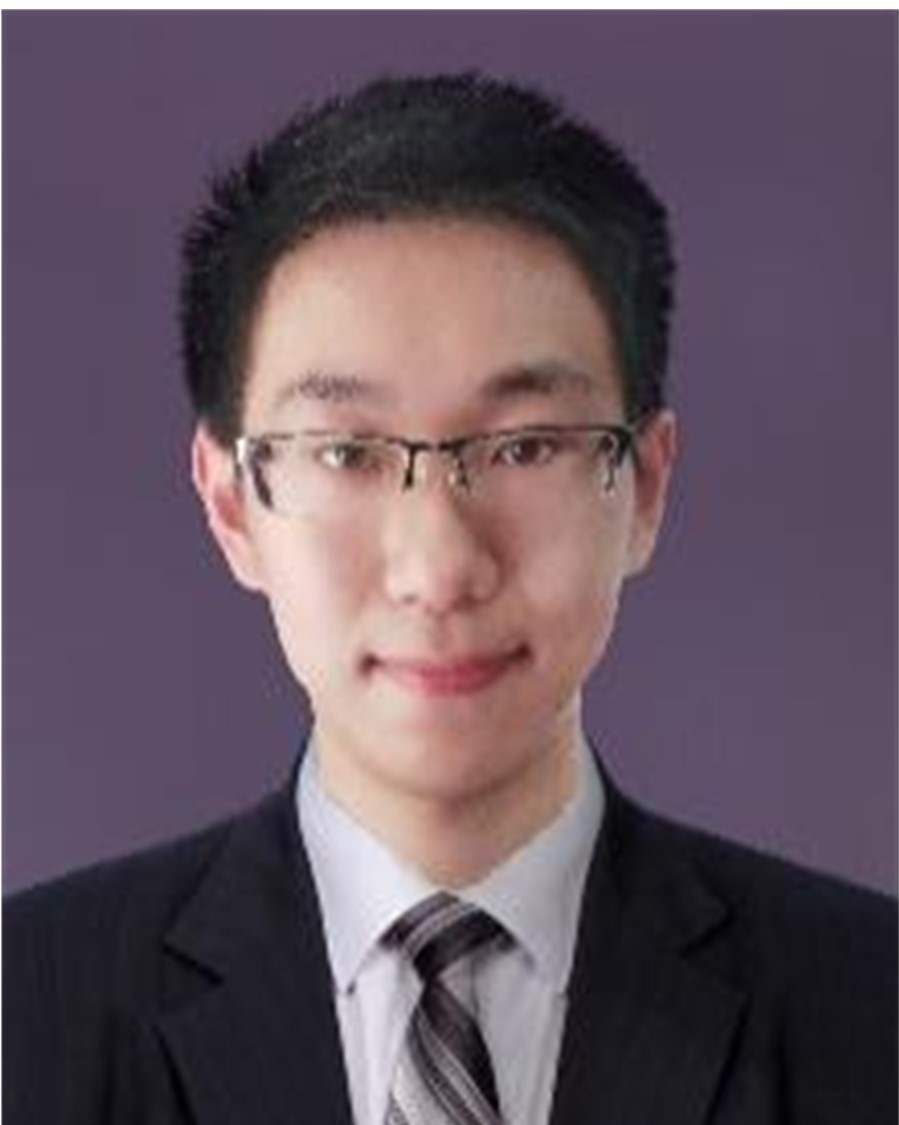
\includegraphics[width=1in,height=1.25in,clip,keepaspectratio]{fig/XiaojingQI.jpg}}]{Xiaojing Qi}
was born in 2000. He received his B.S. degree from Jilin University, Jilin, China, in 2023. He is pursuing his master’s degree in vehicle engineering at the School of Vehicle and Mobility, Tsinghua University, Beijing, China. His research interests include automotive computational fluid dynamics, and vehicle simulation and control, especially regarding the rollover stability control of tank trucks under cloud control systems, cloud-based predictive lane change control, cloud-based predictive cruise control, and cloud control architecture.

E-mail: qxj23@mails.tsinghua.edu.cn
\end{IEEEbiography}
\vspace{-1.2cm}

\begin{IEEEbiography}[{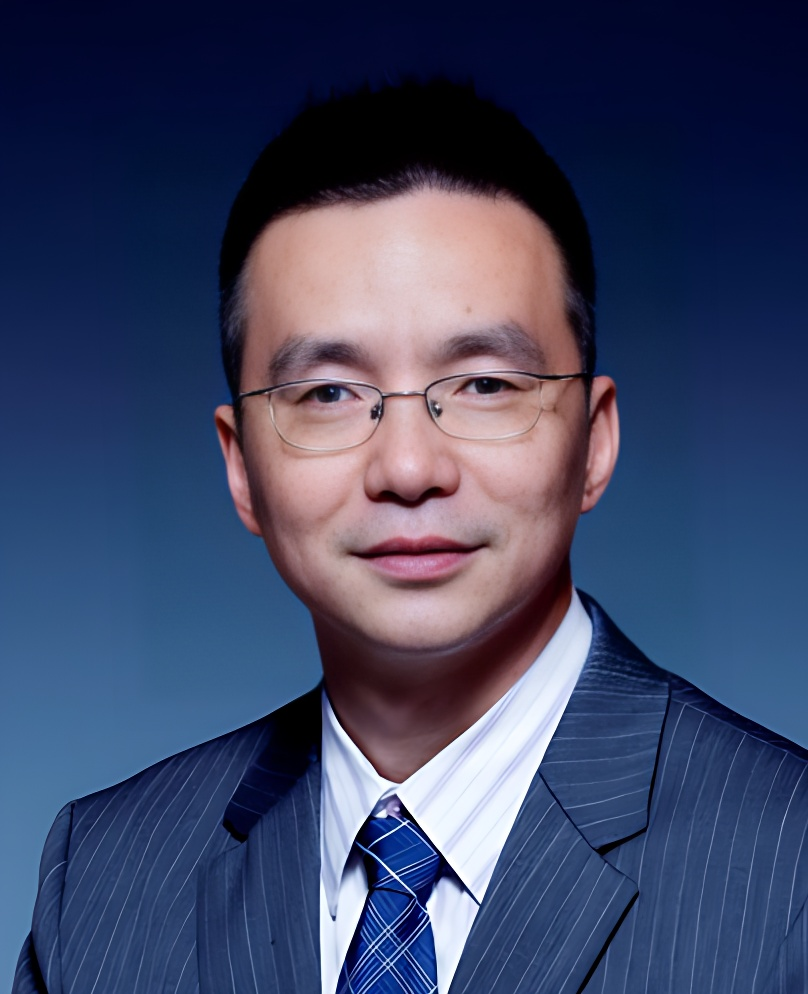
\includegraphics[width=1in,height=1.25in,clip,keepaspectratio]{fig/YugongLUO.png}}]{Yugong Luo}
received the B.S. and M.S. degrees in mechanical engineering from Chongqing University, Chongqing, China, and the Ph.D. degree in mechanical engineering from Tsinghua University, Beijing, China, in 1996, 1999, and 2003, respectively.

He is currently a Professor with the School of Vehicle and Mobility, Tsinghua University. He was a Visiting Scientist with the Department of Mechanical Engineering, University of Michigan Ann Arbor, MI, USA, in 2013 and 2014. He is a coauthor of four books. His research interests include intelligent vehicles, hybrid electric vehicles, and multiobjective control.

E-mail: lyg@tsinghua.edu.cn 
\vspace{-1.2cm}
\end{IEEEbiography}


\begin{IEEEbiography}[{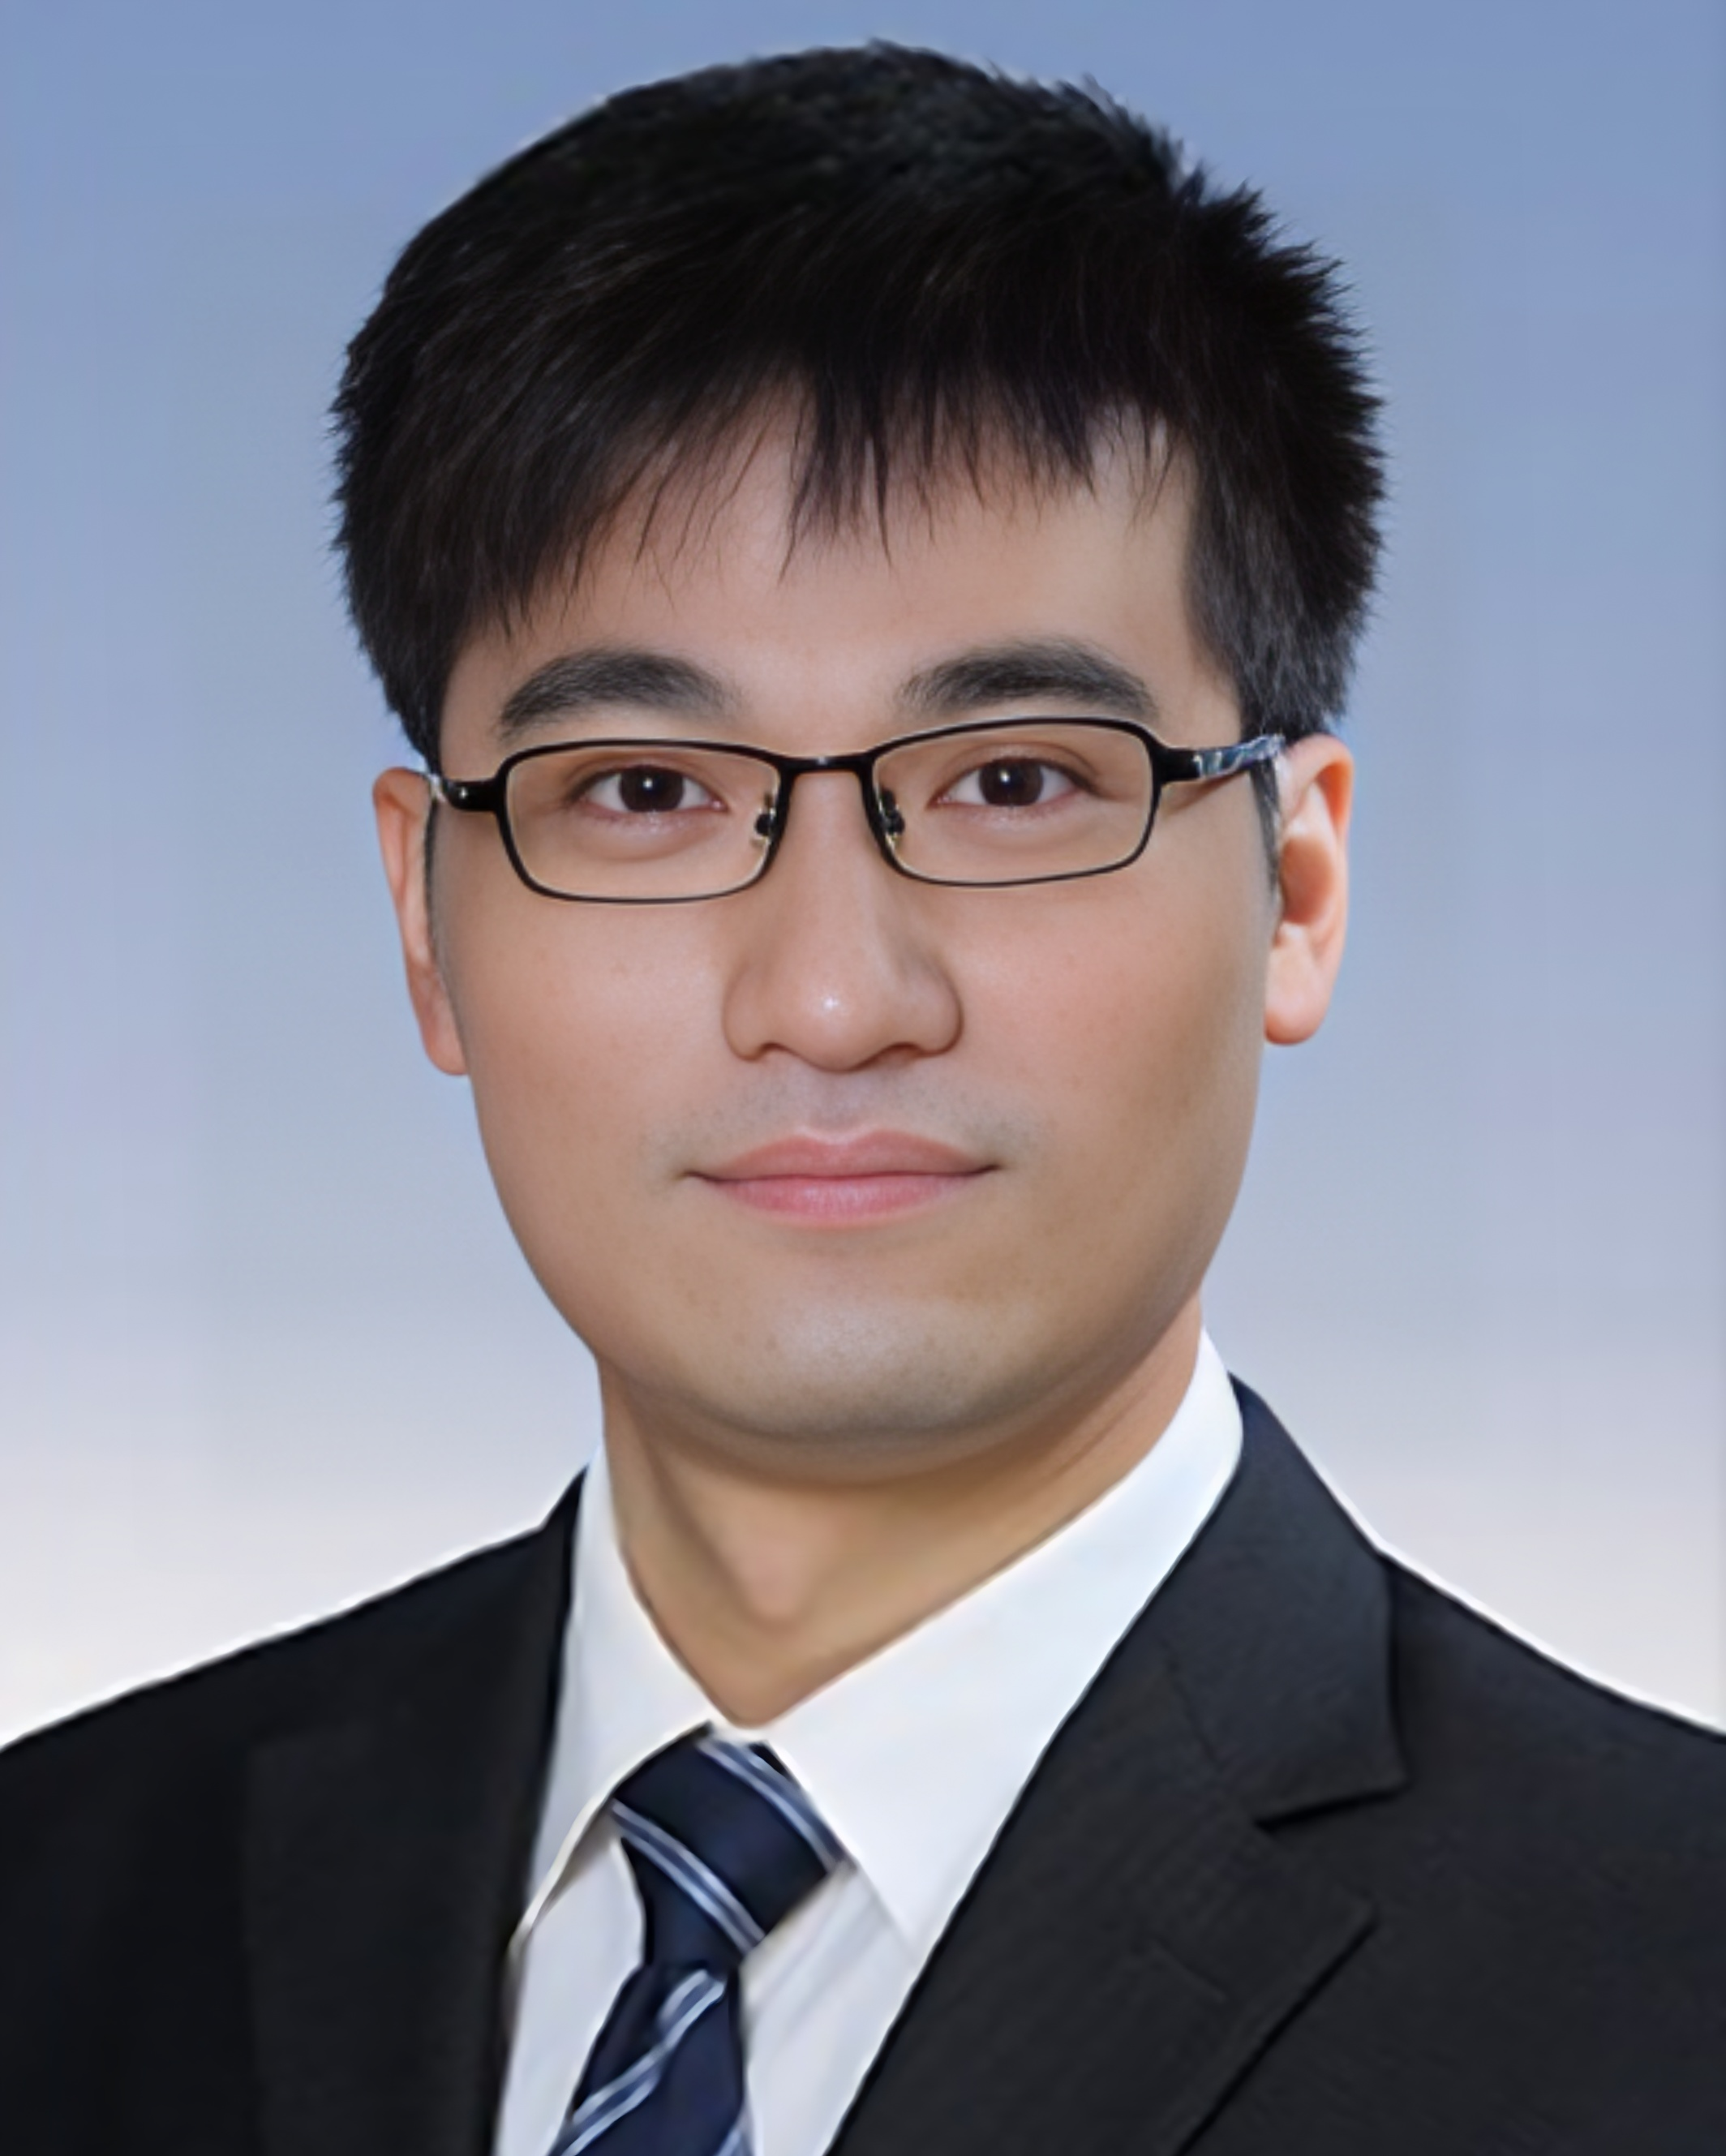
\includegraphics[width=1in,height=1.25in,clip,keepaspectratio]{fig/BolinGAO.jpg}}]{Bolin Gao}
was born in 1986. He is now an associate research professor at the School of Vehicle and Mobility, Tsinghua University. His research interests include the theoretical research and engineering application of the dynamic design and control of intelligent and connected vehicles, especially about the collaborative perception and tracking method in cloud control systems, intelligent predictive cruise control systems on commercial trucks with cloud control mode, as well as the test and evaluation of intelligent vehicle driving systems.

E-mail: gaobolin@tsinghua.edu.cn
\vspace{-1.2cm}
\end{IEEEbiography}

\begin{IEEEbiography}[{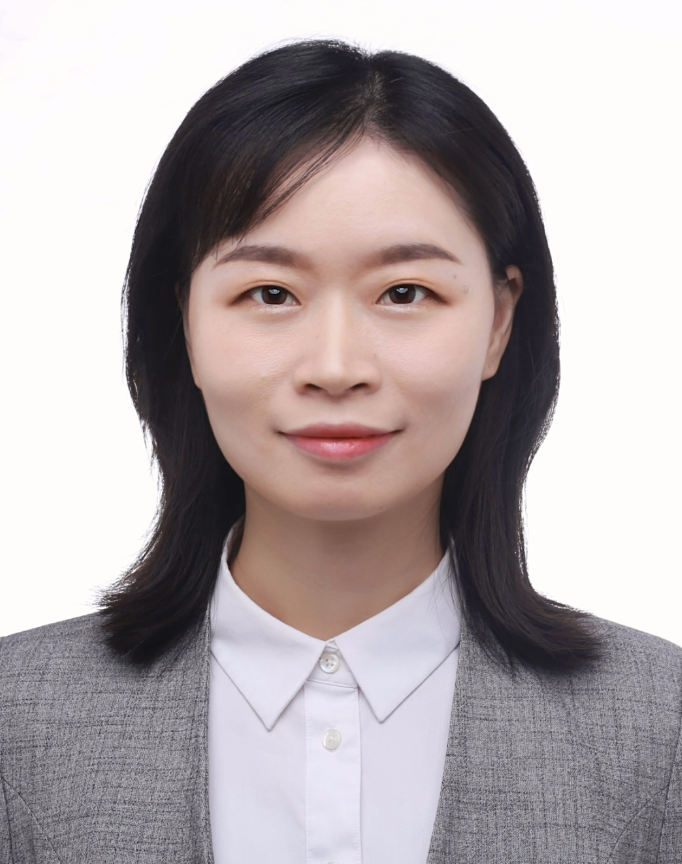
\includegraphics[width=1in,height=1.25in,clip,keepaspectratio]{fig/zhongwei.png}}]{Wei Zhong} received the B.S. and Ph.D. degrees in the School of Vehicle and Mobility, Tsinghua University, China, and used to be the chief at the National Innovation Center of Intelligent and Connected Vehicles, China. She is now an associate research professor at the School of Vehicle and Mobility, Tsinghua University. Her primary research focus is on the integrated design of vehicle-road-cloud integrated control systems, collaborative planning and control, systems engineering, and multi-objective optimization.

E-mail: zhongwei@mail.tsinghua.edu.cn
\end{IEEEbiography}


\vfill

\end{document}




